% ============================================================
%  Seminar deck 
%  Docs: 
% D1 Andrea wtp-wta gap
% D2 Andrea hedonic (toothpaste; functionality; elasticity)
% D3 Runping 6/19 (LLM attention; gap)
% D4 Runping 4/2 (mechanism/mediation)
% ============================================================

\documentclass[10pt]{beamer}   % 4:3
\usepackage{booktabs}
\providecommand{\sym}[1]{\ensuremath{^{#1}}}
\newcommand{\se}[1]{{\scriptsize(#1)}}
\providecommand{\normal}{\normalsize}
\providecommand{\midskip}{\medskip}
\setbeamertemplate{navigation symbols}{}
\setbeamertemplate{footline}{%
  \leavevmode%
  \hbox{%
    \hfill%
    \usebeamerfont{page number in head/foot}%
    \usebeamercolor[fg]{page number in head/foot}%
    \insertframenumber\hspace{1em}%
  }%
  \vskip2pt%
}
\usepackage{fancyvrb}
\usepackage{graphicx}
\newcommand{\ph}[2][0.42\textheight]{%
  \begin{center}%
    \setlength{\fboxsep}{8pt}%
    \fcolorbox{gray!50}{gray!8}{%
      \parbox[c][#1][c]{0.85\linewidth}{\centering\color{gray}\footnotesize FIGURE\\[3pt]#2}}%
  \end{center}}
\newcommand{\src}[1]{\par\smallskip{\footnotesize\color{gray}#1}}
\newcommand{\backbutton}[1]{\hfill\hyperlink{#1}{\beamerbutton{$\blacktriangleleft$ Back}}}
\usepackage[most]{tcolorbox}

% ---- prompt box style ----
\tcbset{
  promptbox/.style={
    enhanced, breakable, colback=gray!3, colframe=black!55,
    boxrule=0.4pt, arc=3pt, left=12pt, right=12pt, top=10pt, bottom=10pt,
    borderline west={2.5pt}{0pt}{black!45},
    fonttitle=\bfseries\sffamily\small, coltitle=white, colbacktitle=black!55,
    attach boxed title to top left={xshift=10pt, yshift=-\tcboxedtitleheight/2},
    boxed title style={arc=2pt, boxrule=0pt},
  }
}

\title{Price Elasticity and Context}

\date{\today}

\begin{document}

\begin{frame}[plain]\titlepage\end{frame}
\begin{frame}{Outline}\tableofcontents\end{frame}

% ============================================================
\section{Motivation}
% ============================================================

\begin{frame}{The big questions}
  \begin{itemize}
    \item How stable are products' valuation and price elasticity across different contexts?
    \item When framing changes valuation and choice, is this because consumers attend to different product attributes?
    \item Can the same framework help explain both instability across contexts and heterogeneity across consumers?
  \end{itemize}
\end{frame}

\begin{frame}{Framing: two reference papers}
  \begin{columns}[T]
    \column{0.48\textwidth}
    \textbf{Wakefield and Inman (2003)}
    \begin{itemize}
      \item Price sensitivity is not a fixed parameter.
      \item It varies with the consumption situation.
      \item Hedonic vs.\ functional use and social context can shift elasticity.
    \end{itemize}

    \column{0.48\textwidth}
    \textbf{Rick, Cryder, and Loewenstein (2008)}
    \begin{itemize}
      \item Consumers differ in the pain of paying.
      \item A thrift/tightwad dimension can shape willingness to spend.
      \item This heterogeneity need not coincide with income or wealth.
    \end{itemize}
  \end{columns}

  \vspace{0.3cm}
  \begin{itemize}
    \item Bottom line: context can shape what the consumer attends to, generating both instability and heterogeneity in product valuation and choice.
  \end{itemize}
\end{frame}

\begin{frame}{Two goods}
  \hypertarget{main:two_goods}{}
  \begin{itemize}
    \item We study two goods: cookies and toothpaste.
    \item These goods are useful because they differ in their level of functionality/hedonicity (\hyperlink{app:functionality_compare}{functionality histogram}).
    \item Within each good, the key comparison is between a regular and a premium brand
      (\hyperlink{app:cookies_products}{cookies}; \hyperlink{app:toothpaste_products}{toothpaste}).
  \end{itemize}
\end{frame}

% ============================================================
\section{Design}
% ============================================================

\begin{frame}{Three key treatments}
  \begin{itemize}
    \item Binary choice: between-subject comparison of Control, Buying, and Consumption; participants choose directly between the regular and premium option at posted prices.
    \item WTP within: within-subject MPL elicitation for both brands; each participant reports a valuation for the premium brand and for the regular brand.
    \item WTA strong: MPL elicitation for the premium brand only; in the current pilot, this is available for cookies but not yet for toothpaste.
  \end{itemize}
  % \ph[0.28\textheight]{task summary table}
  % \src{D1 Table 1/4/App-11; D2 Table 1 for N.}
\end{frame}

\begin{frame}{Measures}
  \begin{itemize}
    \item For both products, we elicit three attention measures:
    \begin{enumerate}

        \item open-text responses, which let us study how participants spontaneously describe the reason for their choice;
        \item a multiple-choice measure that captures the main stated consideration (i.e., price, quality or both);
        \item attention weights, which quantify the relative weight placed on price and quality. \hyperlink{llm_finetune}{\beamerbutton{Fine-Tuning LLM $\blacktriangleright$}}
    \end{enumerate}
    \item For toothpaste only, we also measure functionality/hedonicity.
  \end{itemize}
\end{frame}

\section{Binary}
% ============================================================

\begin{frame}{Binary choice: task structure}
  \begin{itemize}
    \item Participants choose directly between the regular and premium brand at posted prices.
    \item The two options are shown jointly, so the participant makes one side-by-side choice rather than separate valuations.
    \item The design is between-subjects, with three treatment arms: Control, Buying, and Consumption.
    \item The main behavioral outcome is whether the participant chooses the premium option.
  \end{itemize}
\end{frame}

\begin{frame}{Binary choice: treatment arms}
  \hypertarget{main:binary_arms}{}
  \begin{itemize}
    \item Across arms, the posted premium-versus-regular choice is the same; what changes is the treatment framing that precedes or accompanies that choice.
    \item `Control` is the baseline version of the binary choice (\hyperlink{app:manipulation_control}{link}).
    \item `Buying` is one treatment version (\hyperlink{app:manipulation_buying}{link}).
    \item `Consumption` is the other treatment version (\hyperlink{app:manipulation_consumption_cookies}{cookies}; \hyperlink{app:manipulation_consumption_toothpaste}{toothpaste}).
    \item Before choosing, participants describe the image prompt in their own words: what is happening, where, what the person is thinking, and the essence of the situation; they are told there is no right or wrong answer and are encouraged to think carefully and write as much as they would like.
  \end{itemize}
\end{frame}

\begin{frame}{Premium share by treatment}
  \begin{columns}
    \column{0.5\textwidth}\centering Cookies\\[2pt]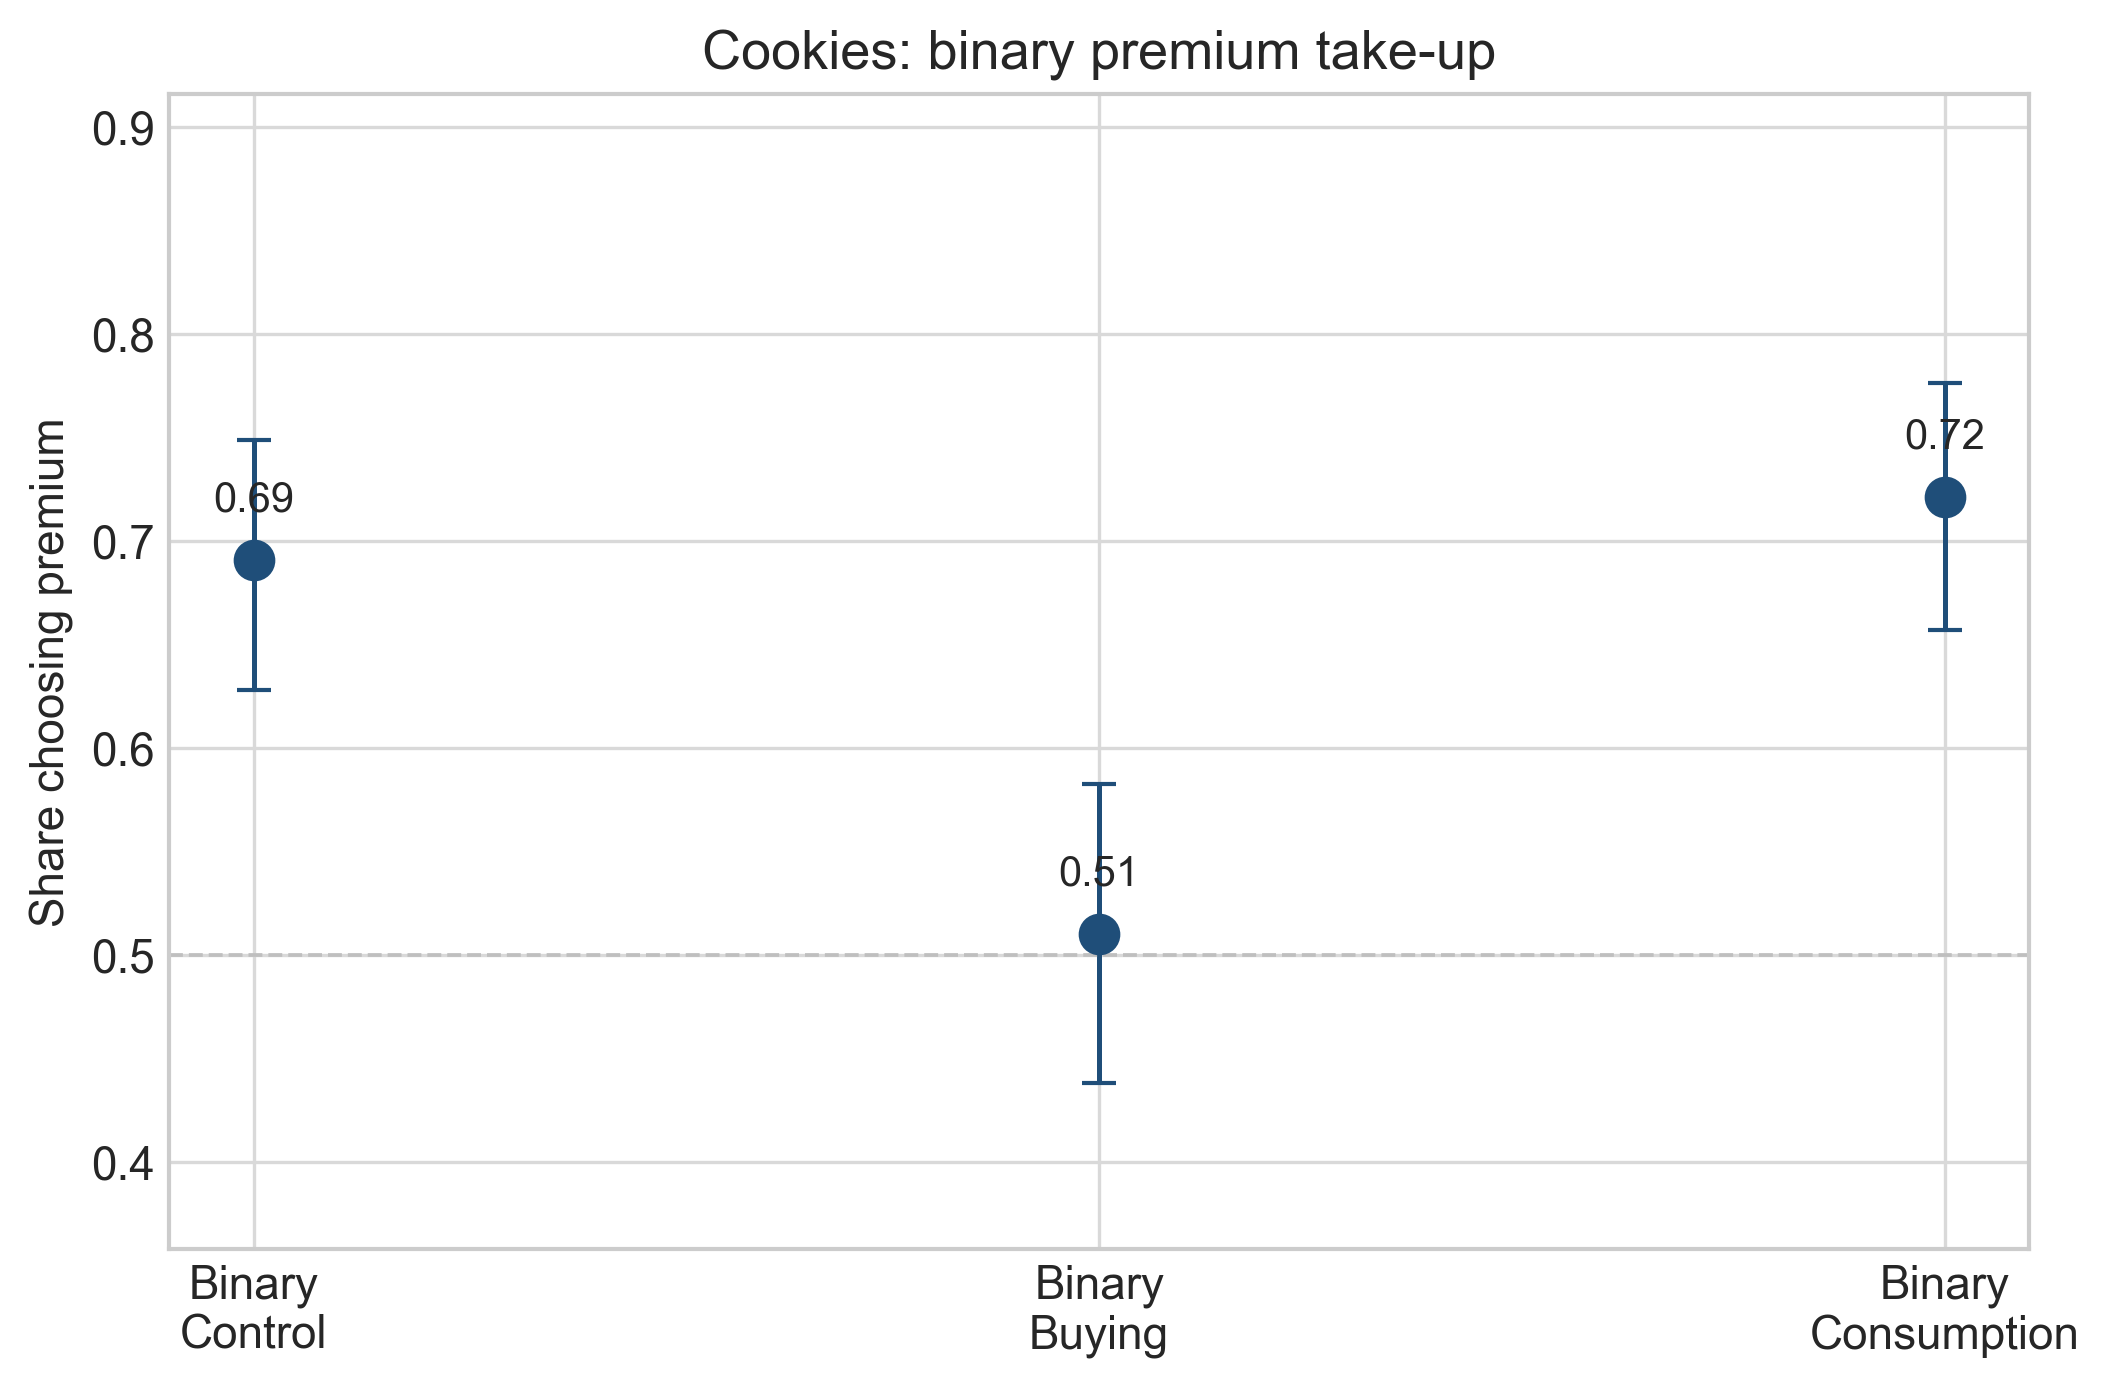
\includegraphics[width=\textwidth]{figures/binary_cookies_premium_share.png}
    \column{0.5\textwidth}\centering Toothpaste\\[2pt]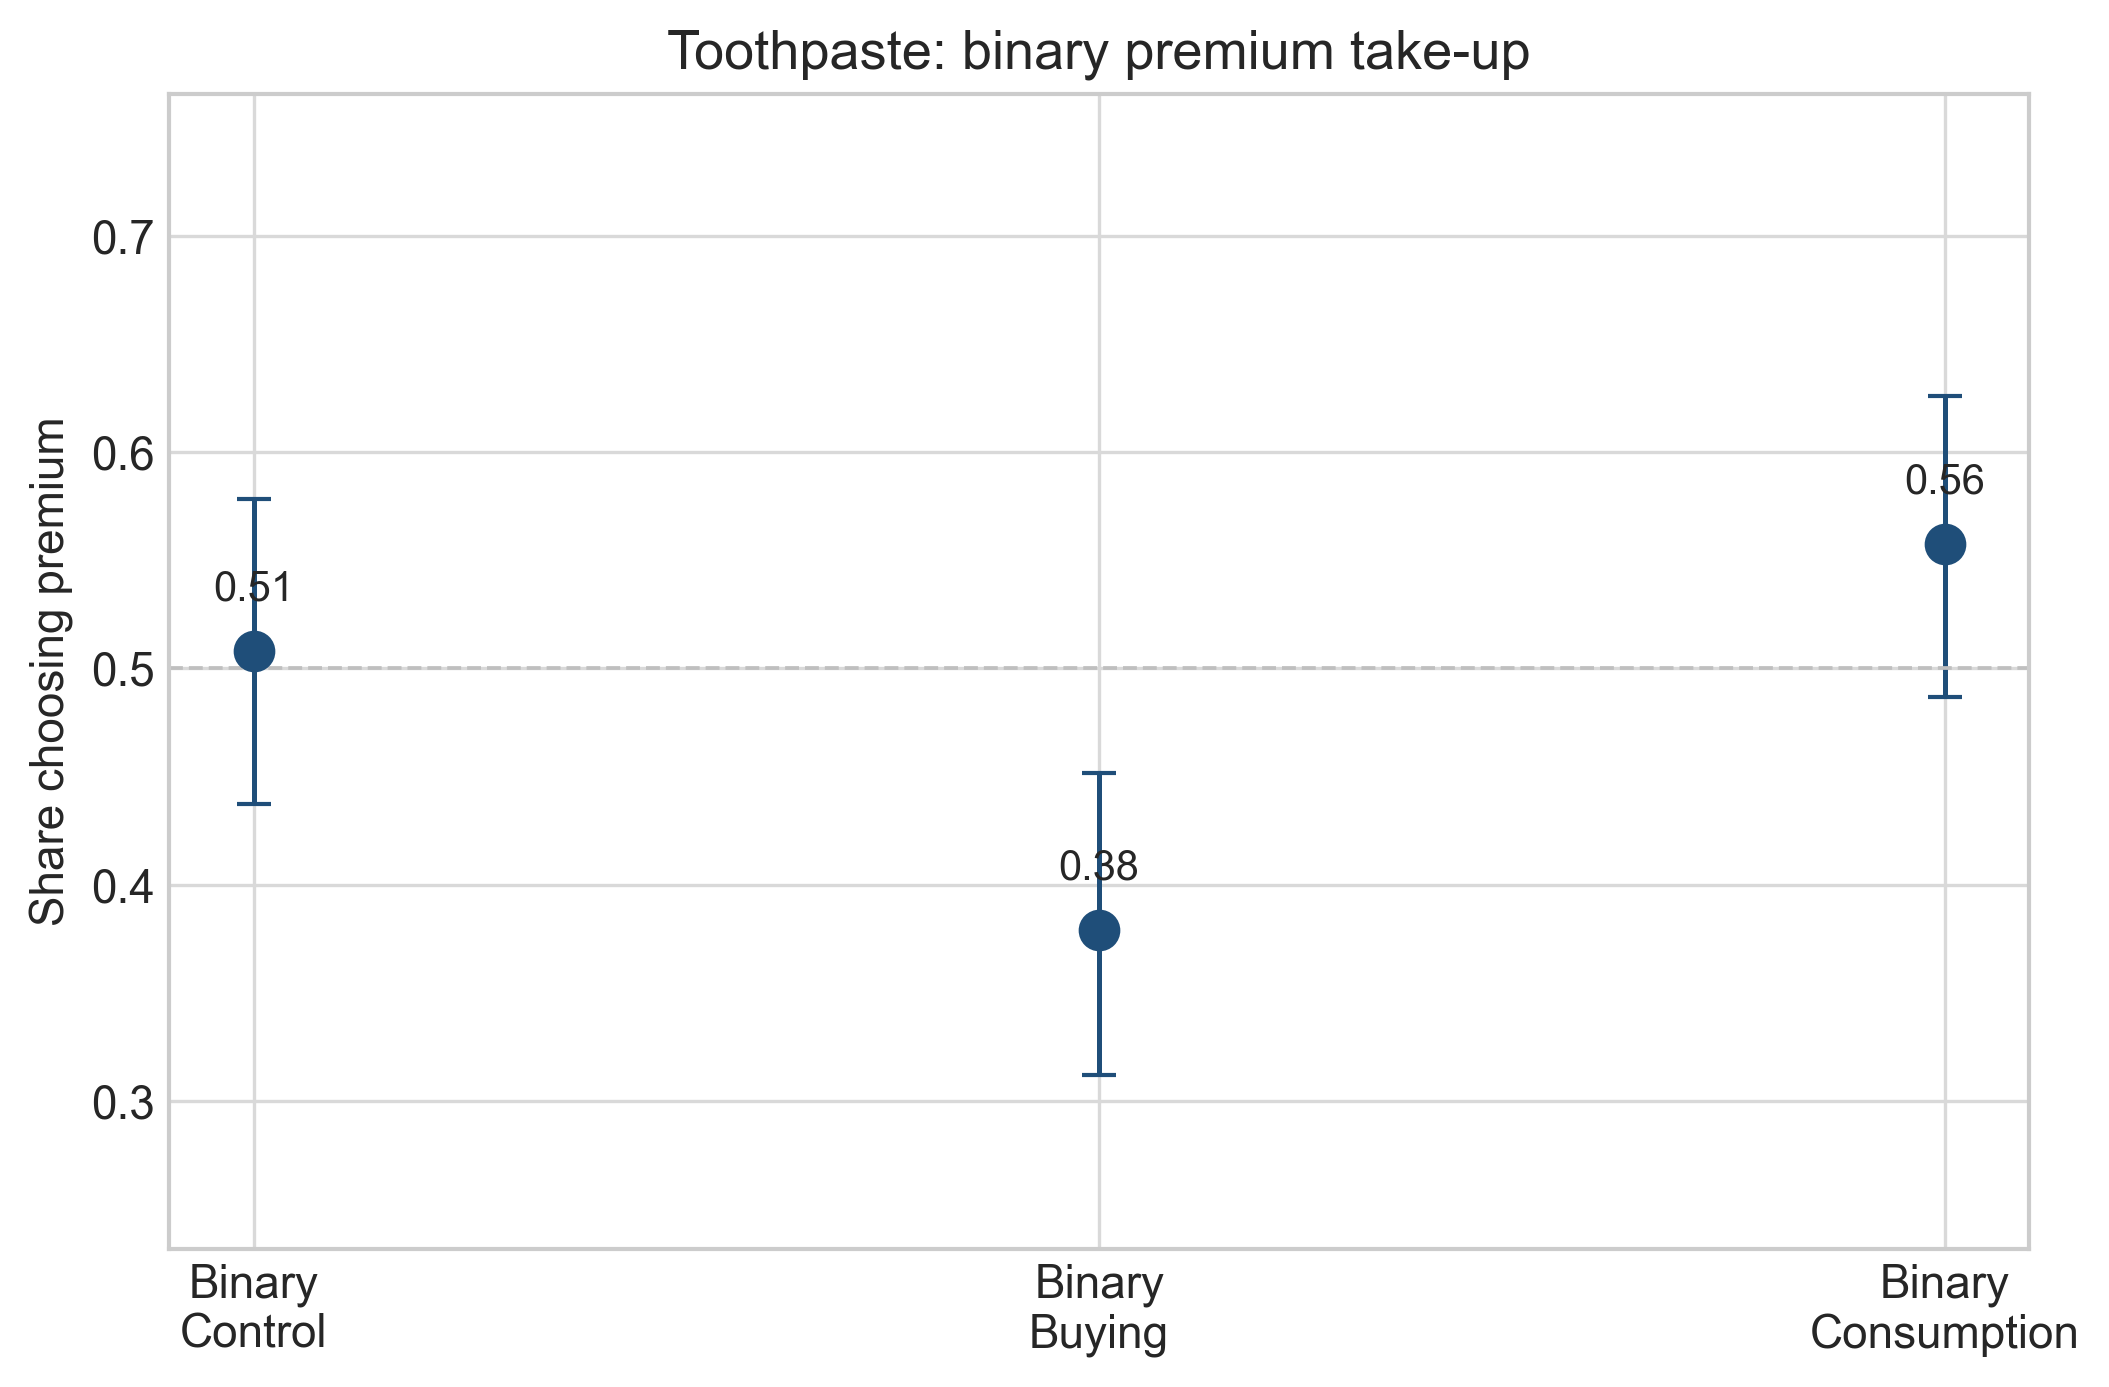
\includegraphics[width=\textwidth]{figures/binary_toothpaste_premium_share.png}
  \end{columns}
\end{frame}

\begin{frame}{Attention and premium share by treatment}
  \hypertarget{main:binary_attention}{}
  \hfill\hyperlink{app:binary_attention_multiple_choice}{\beamerbutton{Multiple-choice version}}
  \medskip
  \begin{columns}
    \column{0.5\textwidth}\centering Cookies\\[2pt]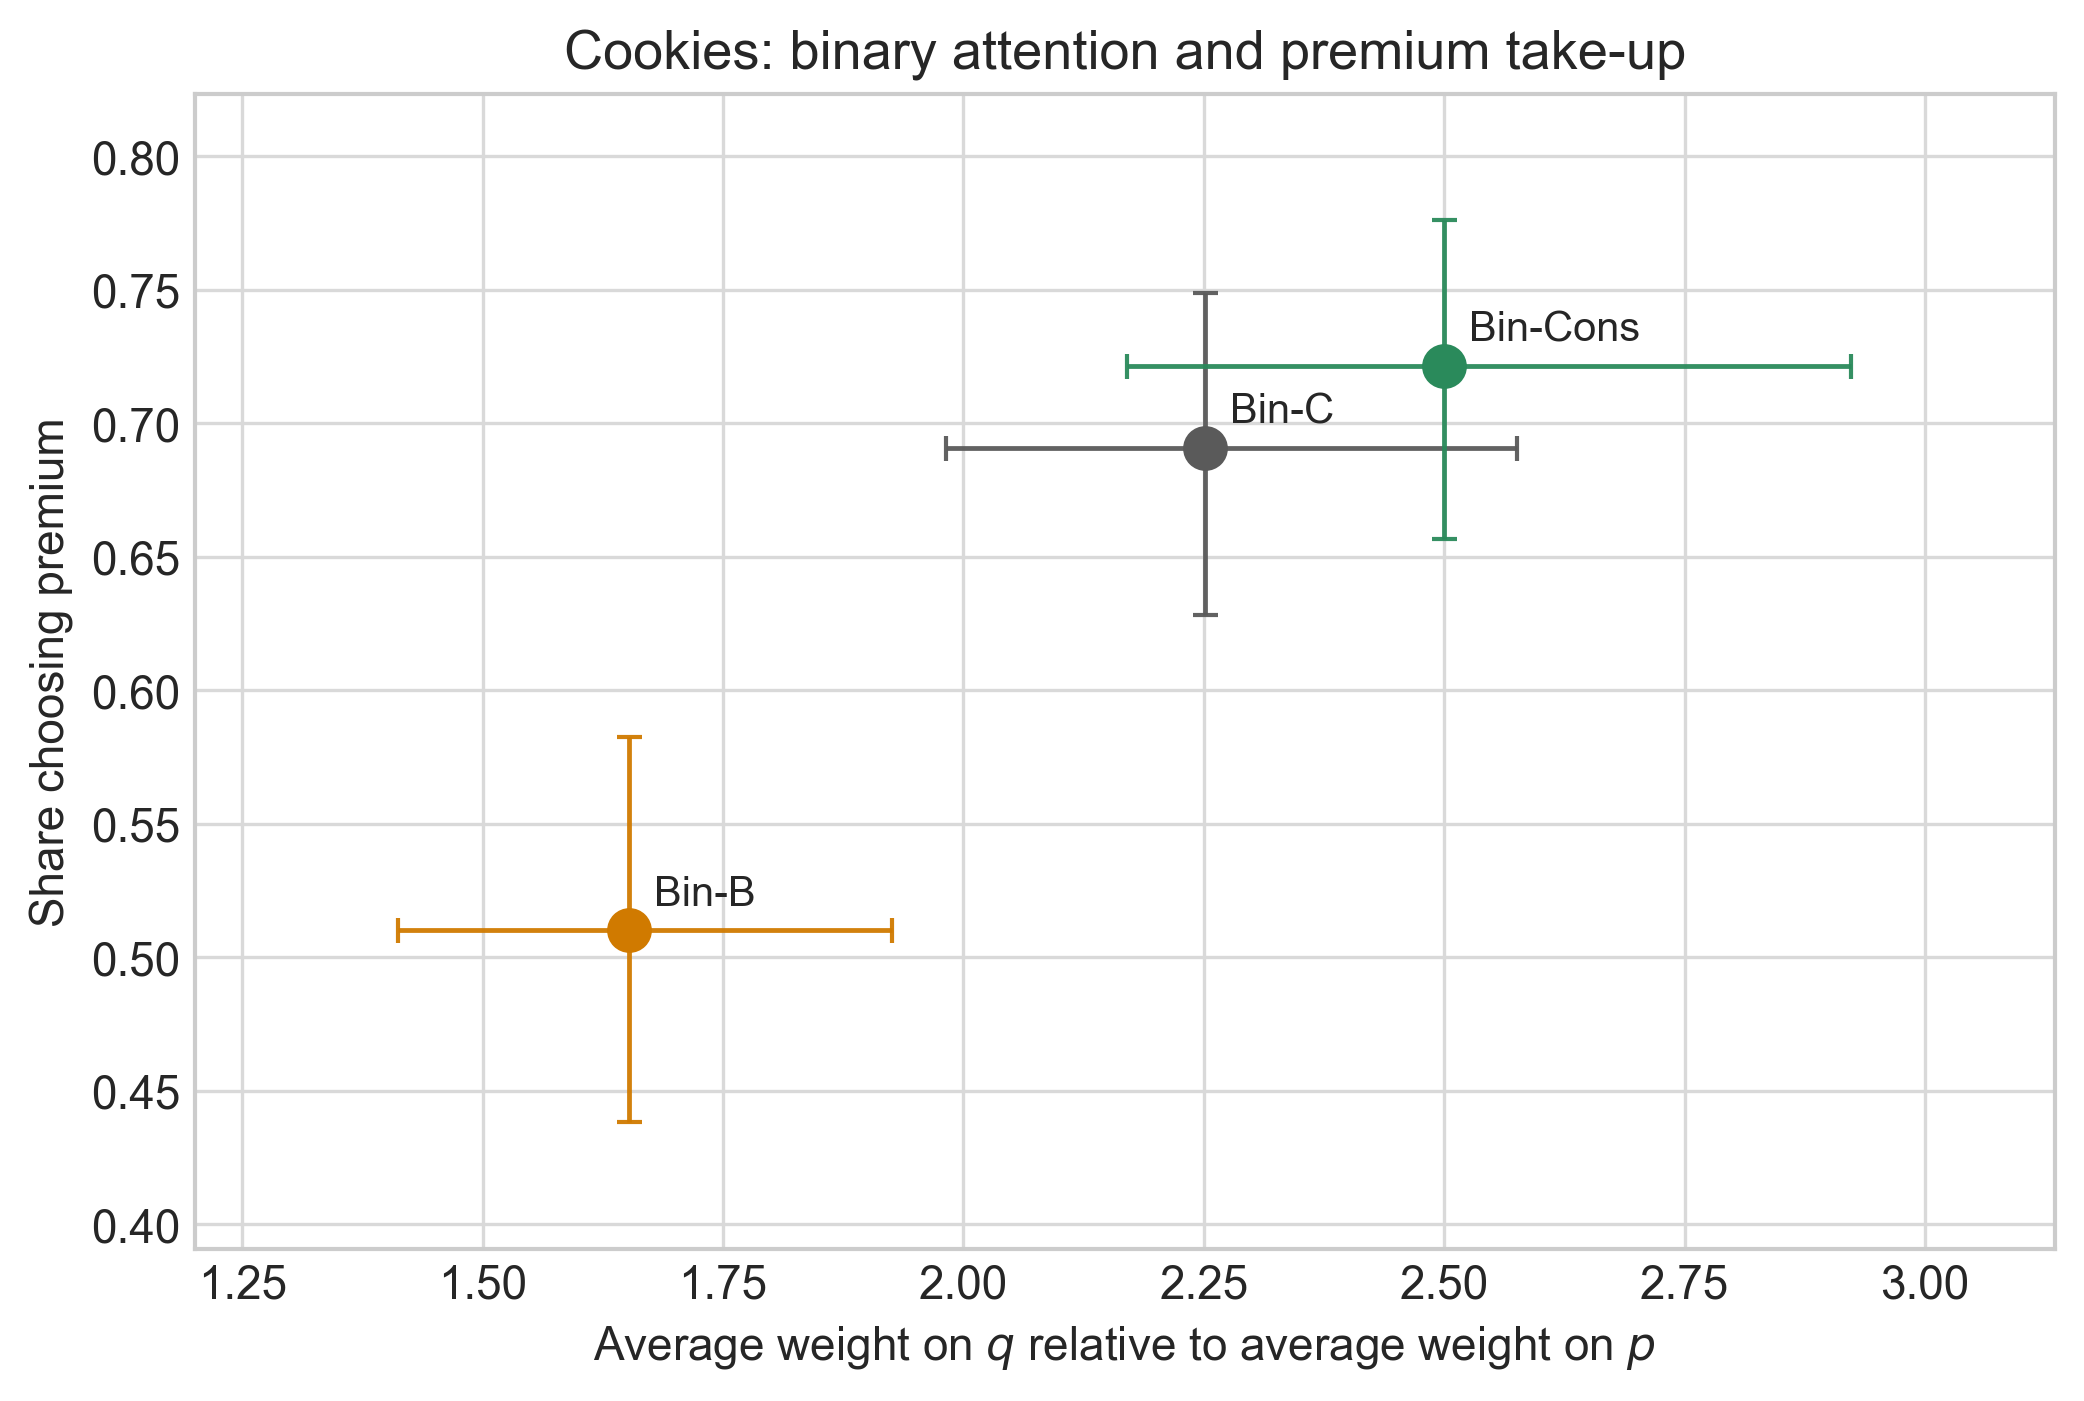
\includegraphics[width=\textwidth]{figures/binary_cookies_attention_vs_premium_share.png}
    \column{0.5\textwidth}\centering Toothpaste\\[2pt]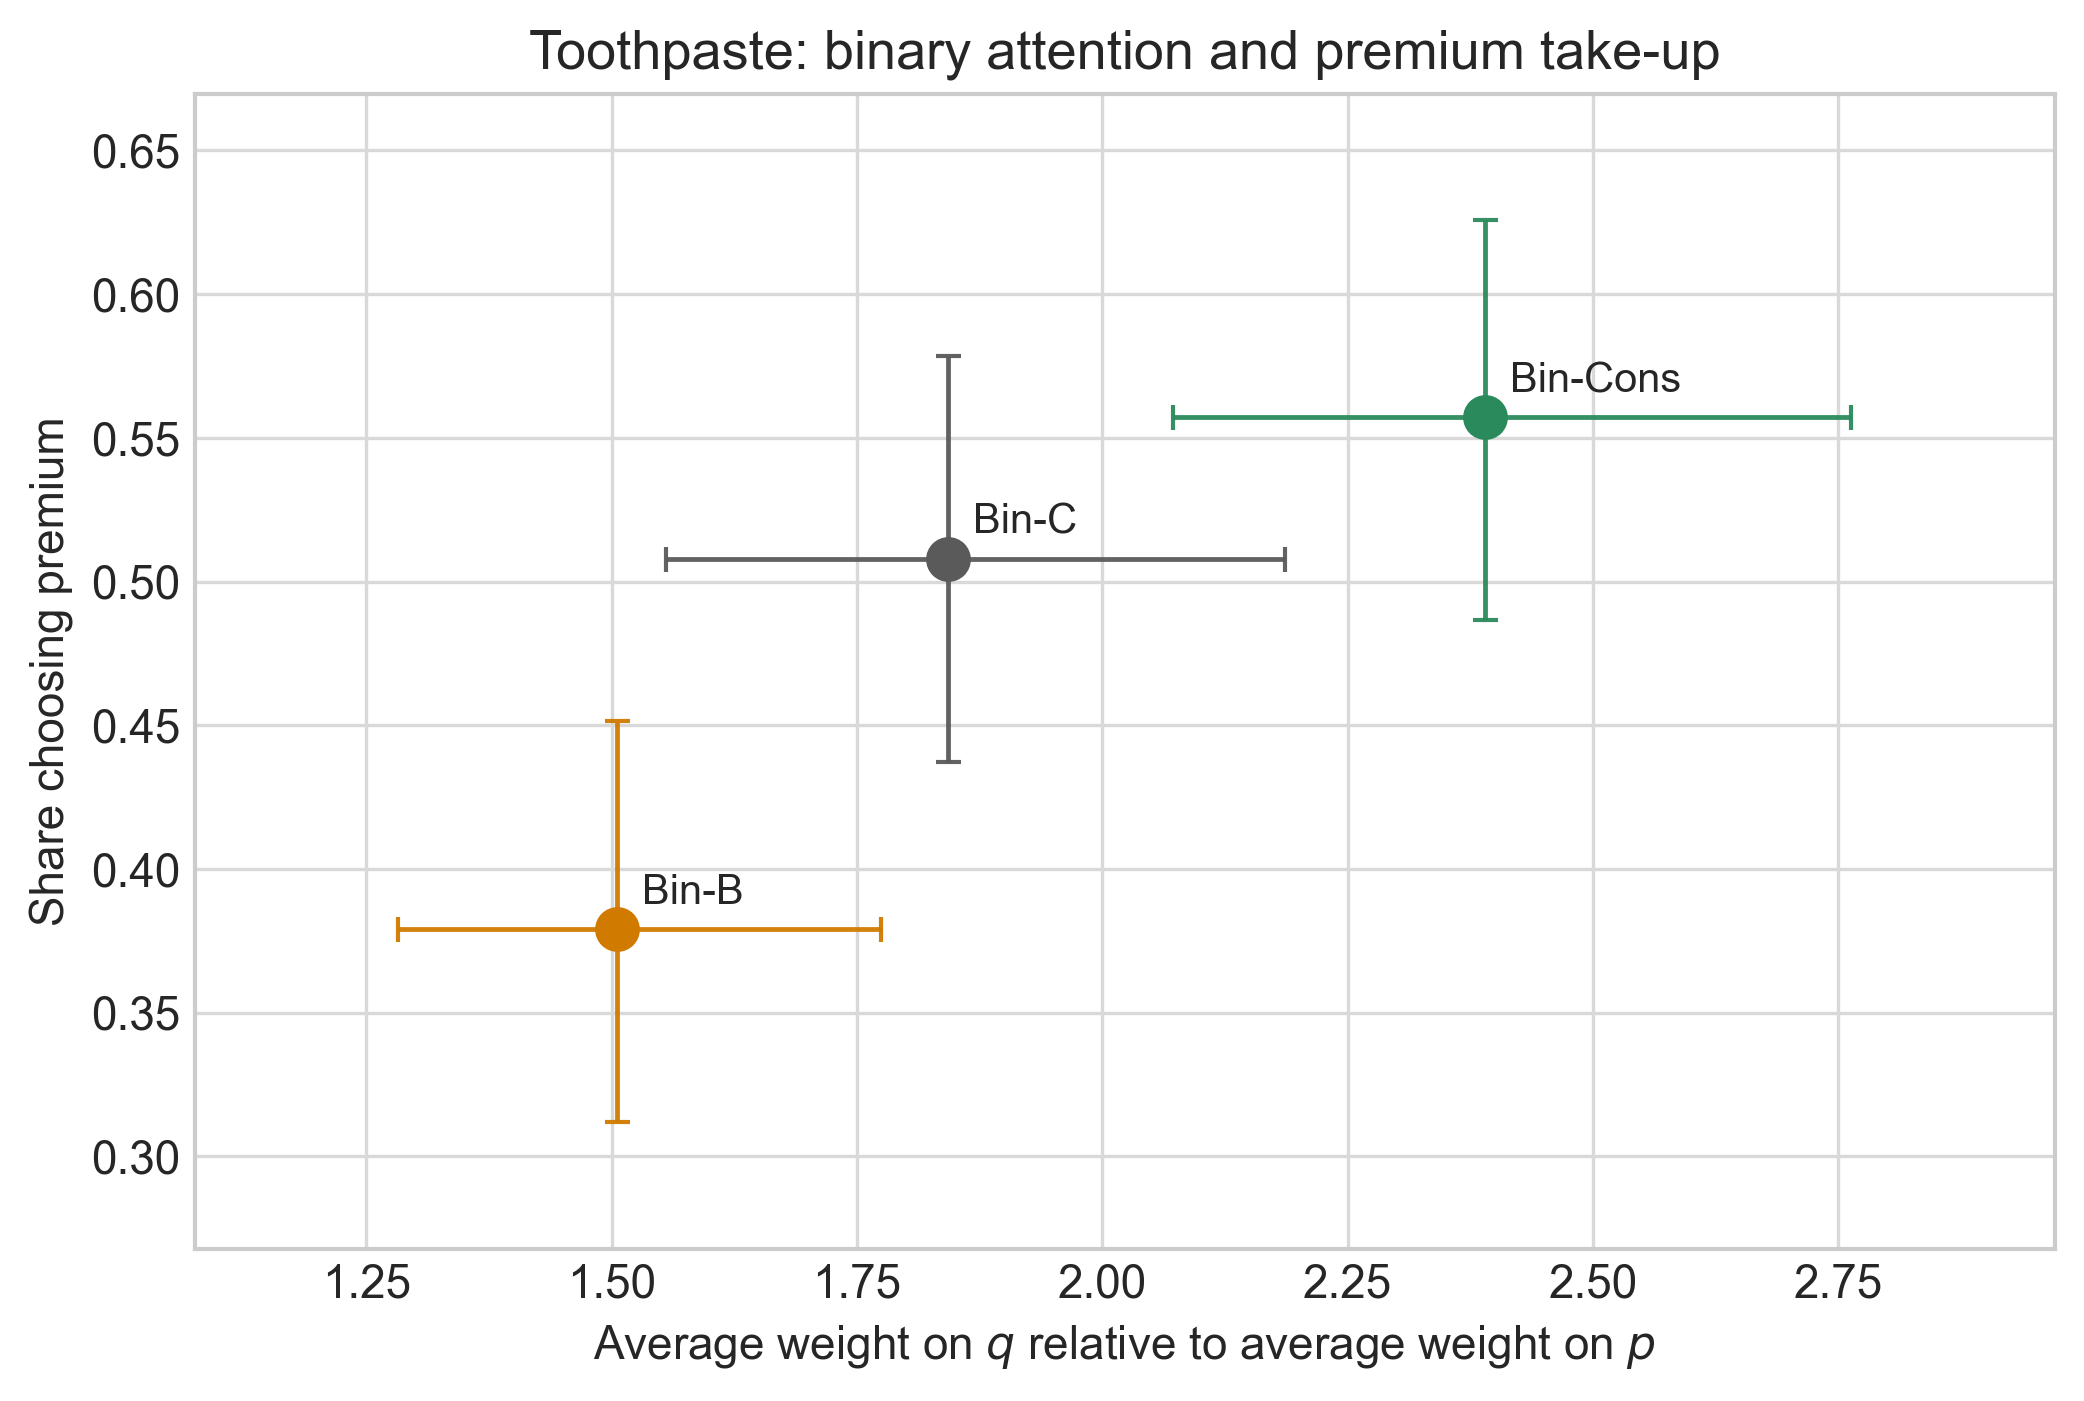
\includegraphics[width=\textwidth]{figures/binary_toothpaste_attention_vs_premium_share.png}
  \end{columns}

\end{frame}




% ============================================================
\section{WTP within}
% ============================================================

\begin{frame}{WTP within: task structure}
  \begin{itemize}
    \item Each participant completes a multiple-price-list task for both brands: one MPL for the premium brand and one MPL for the regular brand.
    \item For each brand separately, the participant moves through a list of prices and indicates whether they would buy at each price.
    \item The task is isolated rather than joint: the premium and regular products are valued separately, not chosen side by side.
    \item In the current comparison, this WTP-within task is the Control benchmark.
  \end{itemize}
\end{frame}

\begin{frame}{WTP within: participant flow}
  \begin{itemize}
    \item The same participant values both brands, so each person generates a premium valuation and a regular valuation.
    \item The order of the two brand-specific MPLs can vary across participants: some see premium first, others regular first.
    \item From those two MPL blocks, we recover the individual premium-minus-regular valuation gap.
  \end{itemize}
\end{frame}

\begin{frame}{WTP within: premium and regular distributions}
  \begin{columns}
    \column{0.5\textwidth}\centering Cookies\\[2pt]
    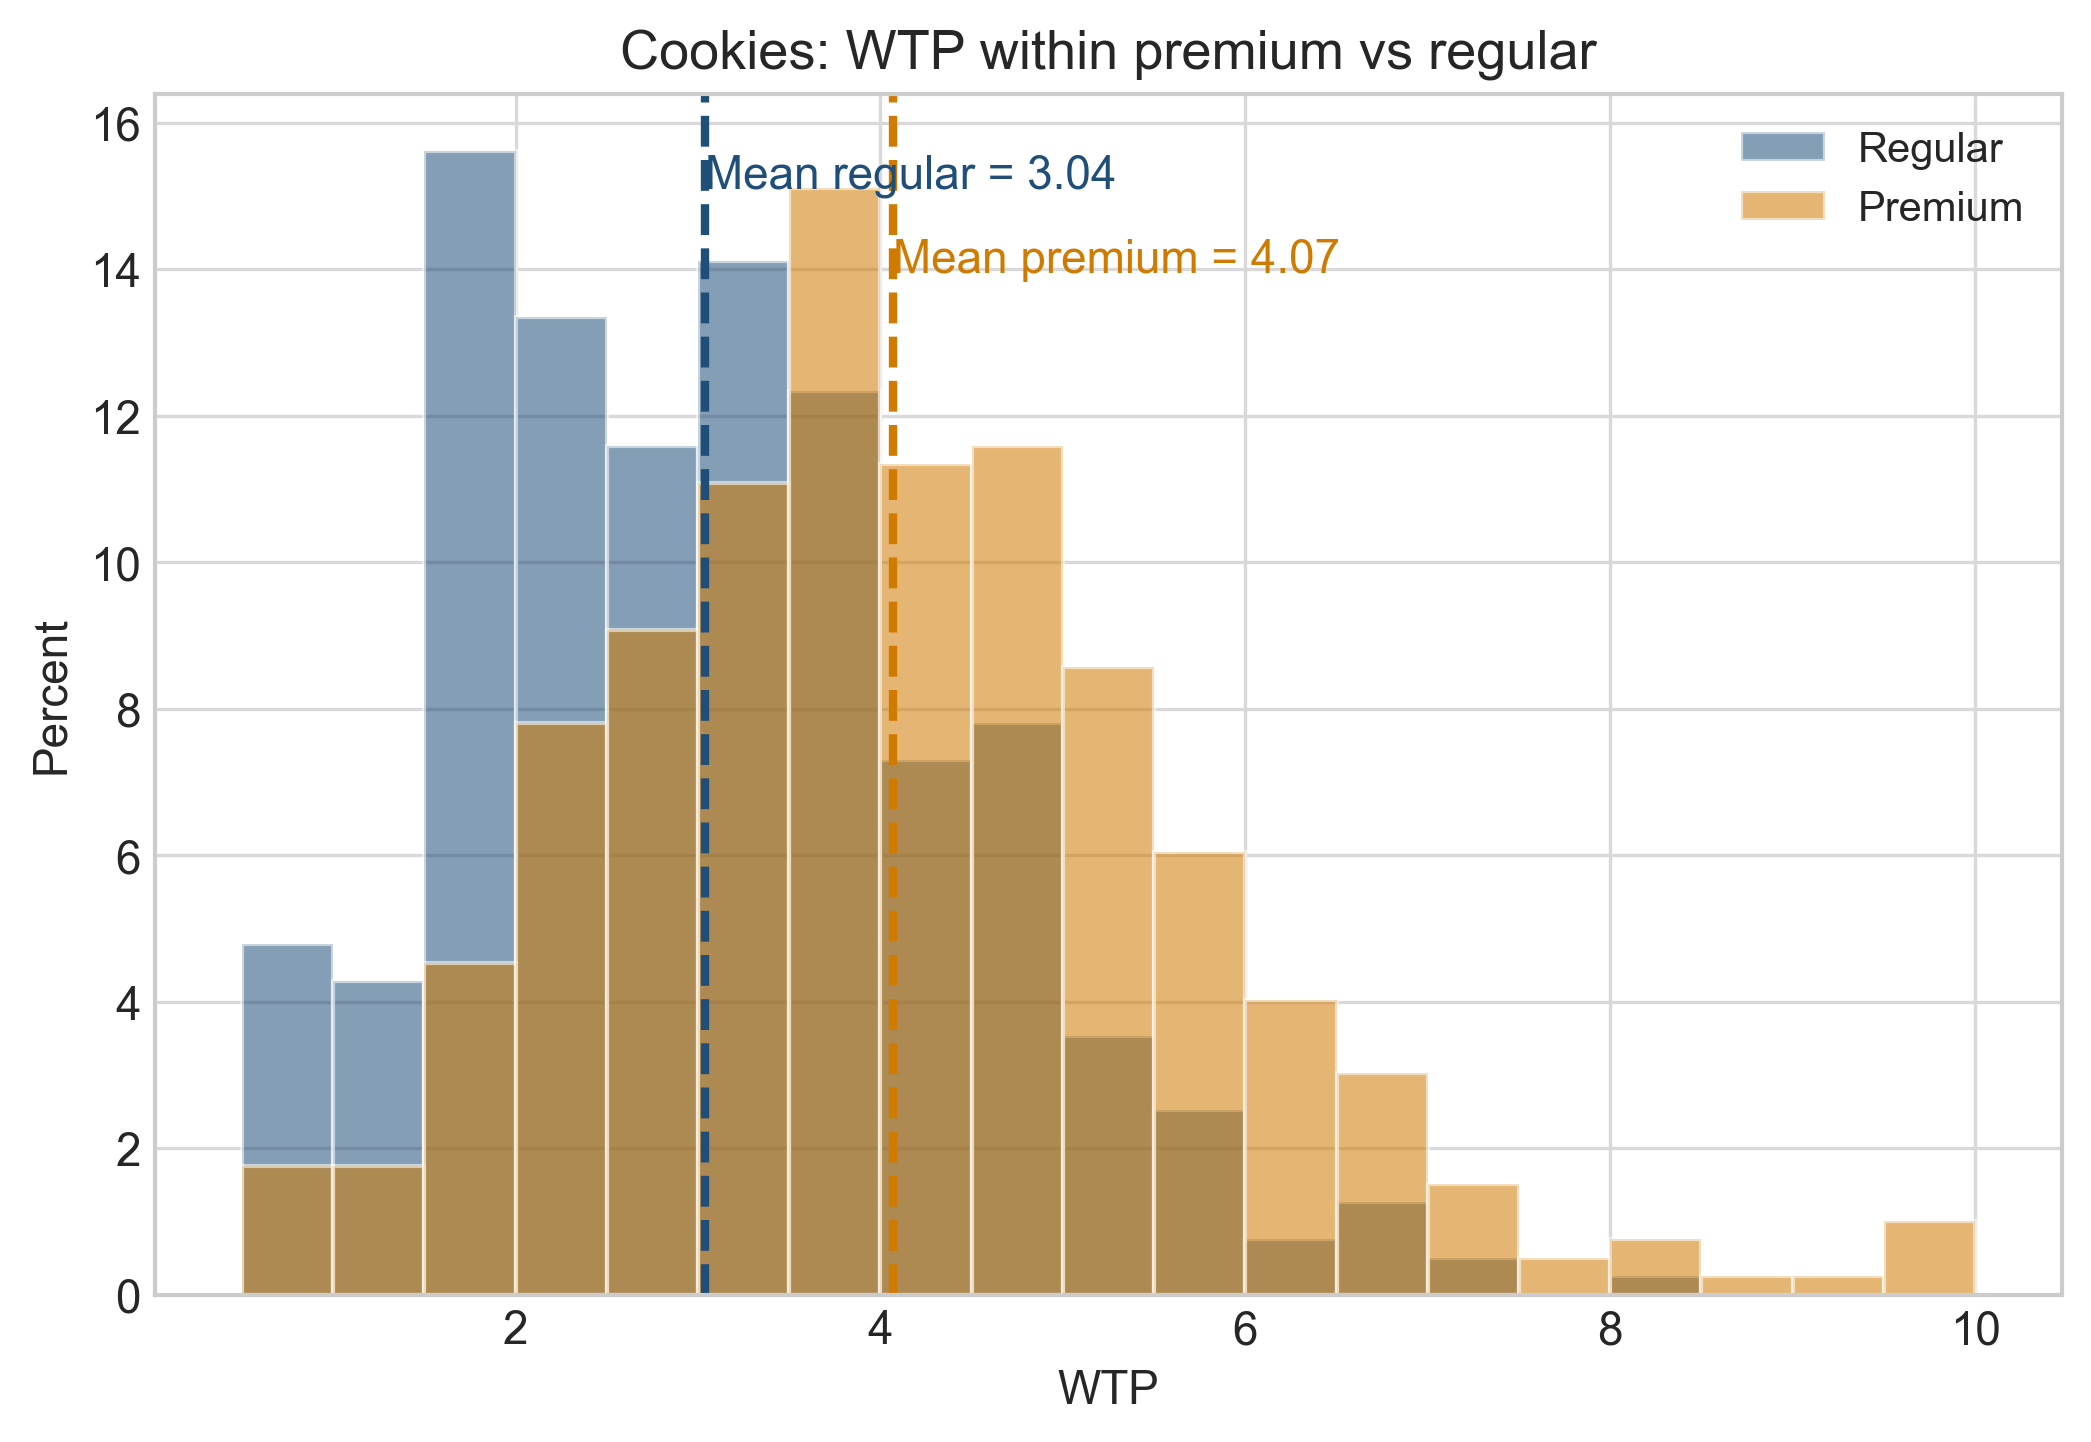
\includegraphics[width=\textwidth]{figures/wtp_within_cookies_distribution.png}

    \column{0.5\textwidth}\centering Toothpaste\\[2pt]
    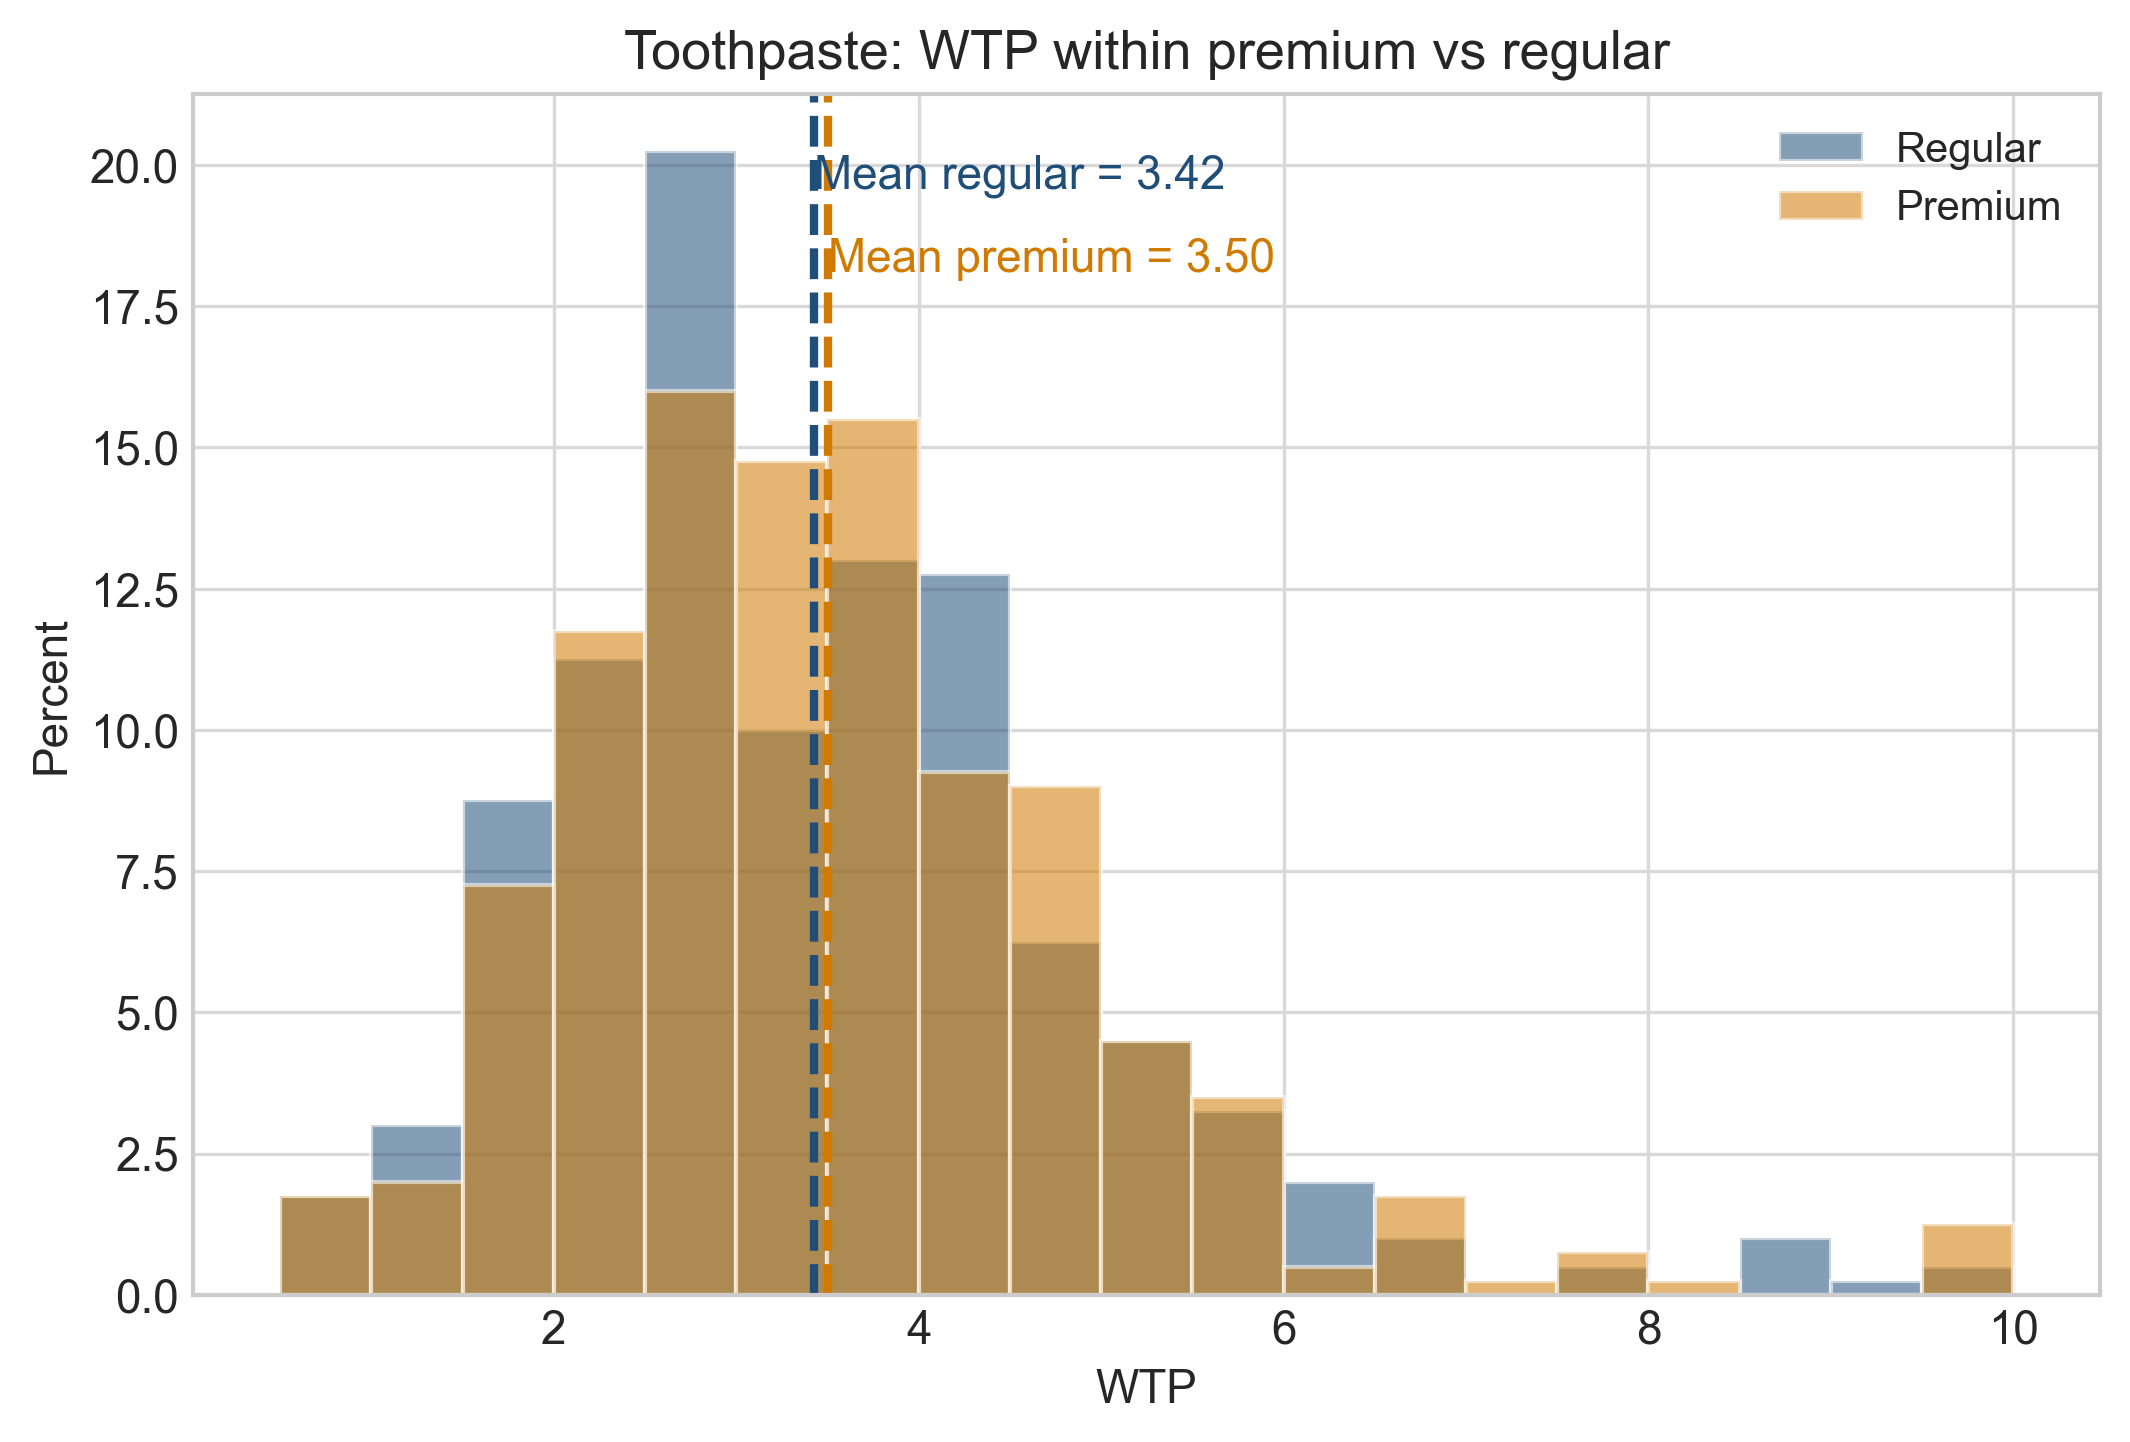
\includegraphics[width=\textwidth]{figures/wtp_within_toothpaste_distribution.png}
  \end{columns}
\end{frame}

\begin{frame}{WTP within: valuations and attention by product}
  \hypertarget{main:wtp_within_attention}{}
  \hfill\hyperlink{app:wtp_within_attention_multiple_choice}{\beamerbutton{Multiple-choice version}}
  \medskip
  \begin{columns}
    \column{0.5\textwidth}\centering Cookies\\[2pt]
    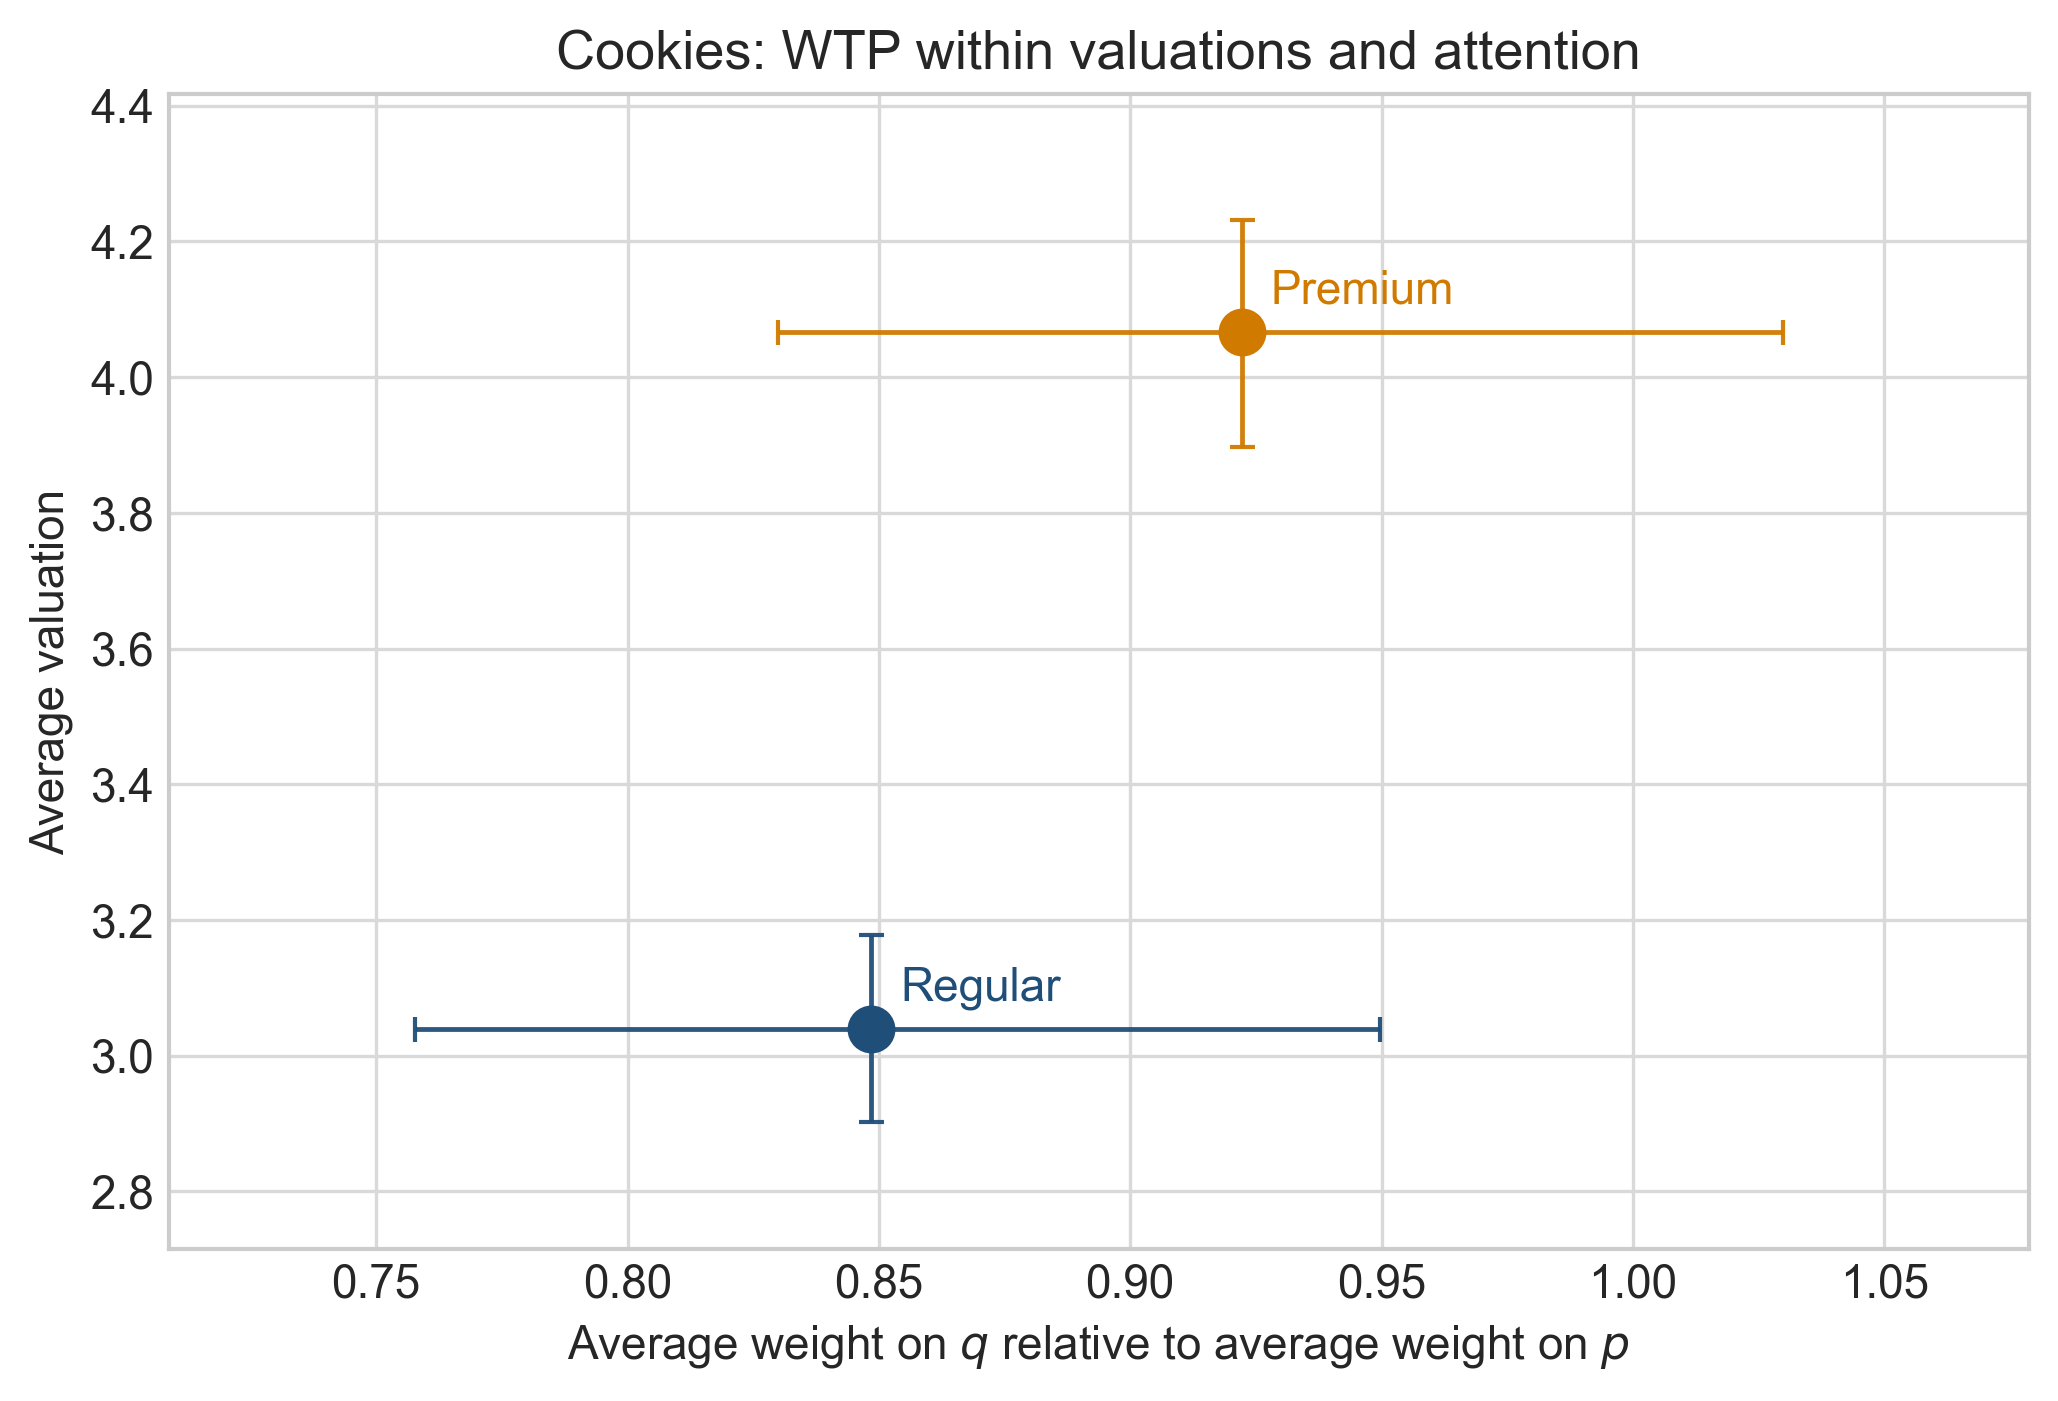
\includegraphics[width=\textwidth]{figures/wtp_within_cookies_ratio_vs_price.png}

    \column{0.5\textwidth}\centering Toothpaste\\[2pt]
    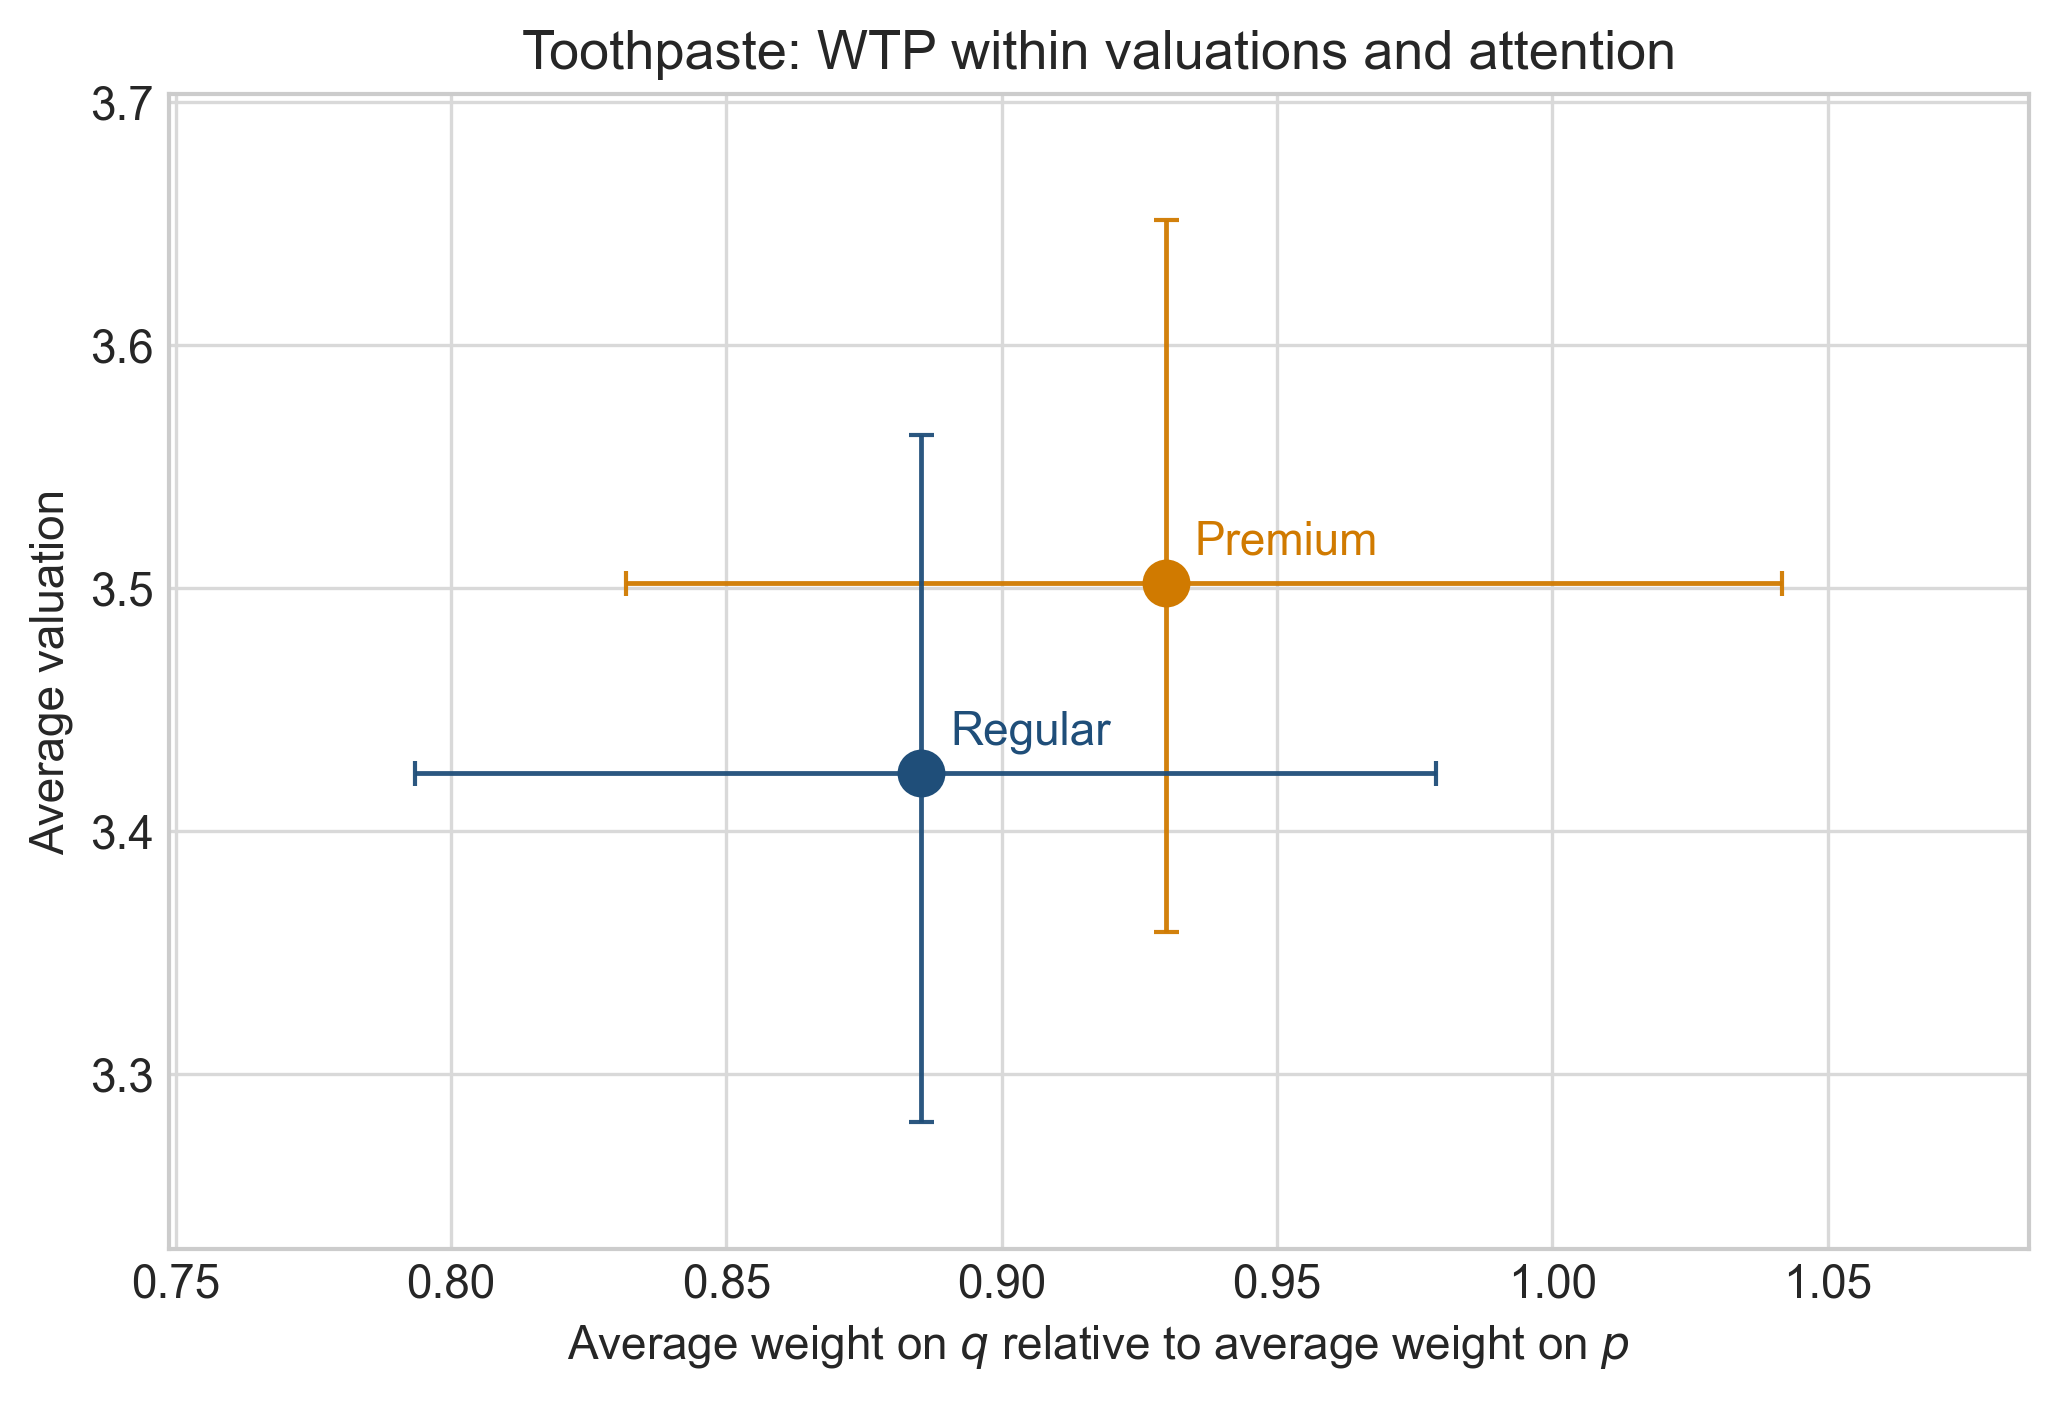
\includegraphics[width=\textwidth]{figures/wtp_within_toothpaste_ratio_vs_price.png}
  \end{columns}
\end{frame}

\begin{frame}{WTP within: attention and valuation gap}
  \hypertarget{main:wtp_gap_reg}{}
  \hfill\hyperlink{app:wtp_takeup_reg}{\beamerbutton{Related take-up table}}
  \medskip

\centering
\tiny
\renewcommand{\arraystretch}{0.92}\setlength{\tabcolsep}{3pt}
\begin{tabular}{@{}l*{7}{c}@{}}
\toprule
 & \multicolumn{7}{c}{Premium $-$ regular WTP gap (\$)} \\
\cmidrule(lr){2-8}
 & (1) & (2) & (3) & (4) & (5) & (6) & (7) \\
\midrule
$\omega^{SR}_p$              & $-0.012$\sym{***} &                    & $-0.013$\sym{***} &                    &                   & $-0.004$          & $-0.007$\sym{**}  \\
                             & (0.003)           &                    & (0.004)           &                    &                   & (0.003)           & (0.004)           \\[1pt]
\addlinespace[2pt]
\multicolumn{8}{@{}l}{Self-reported attention \quad (baseline: Price)} \\
\addlinespace[1pt]
\quad Quality                &                   & $\phantom{-}0.481$\sym{**} & $-0.105$          &                    &                   &                   & $-0.509$\sym{*}   \\
                             &                   & (0.215)            & (0.269)           &                    &                   &                   & (0.278)           \\[1pt]
\quad Both                   &                   & $\phantom{-}0.471$\sym{***} & $\phantom{-}0.207$ &                    &                   &                   & $\phantom{-}0.015$ \\
                             &                   & (0.163)            & (0.170)           &                    &                   &                   & (0.169)           \\[1pt]
$\omega^{LLM}_p$             &                   &                    &                   & $-0.033$\sym{***} & $-0.016$\sym{*}   & $-0.013$          & $-0.015$          \\
                             &                   &                    &                   & (0.005)           & (0.009)           & (0.009)           & (0.009)           \\[1pt]
\addlinespace[2pt]
\multicolumn{8}{@{}l}{LLM labelled attention \quad (baseline: Price Alternatives/Disutility)} \\
\addlinespace[1pt]
\quad Price (Reference Price)&                   &                    &                   &                    & $\phantom{-}0.553$\sym{**} & $\phantom{-}0.539$\sym{*} & $\phantom{-}0.499$\sym{*} \\
                             &                   &                    &                   &                    & (0.272)           & (0.275)           & (0.274)           \\[1pt]
\quad Quality                &                   &                    &                   &                    & $\phantom{-}0.188$ & $\phantom{-}0.177$ & $\phantom{-}0.174$ \\
                             &                   &                    &                   &                    & (0.366)           & (0.364)           & (0.363)           \\[1pt]
\quad Both                   &                   &                    &                   &                    & $\phantom{-}0.264$ & $\phantom{-}0.254$ & $\phantom{-}0.226$ \\
                             &                   &                    &                   &                    & (0.227)           & (0.226)           & (0.224)           \\[1pt]
\addlinespace[2pt]
\multicolumn{8}{@{}l}{LLM labelled valence \quad (baseline: Price Too High)} \\
\addlinespace[1pt]
\quad Quality Too Low        &                   &                    &                   &                    & $-0.585$          & $-0.624$          & $-0.538$          \\
                             &                   &                    &                   &                    & (0.451)           & (0.450)           & (0.439)           \\[1pt]
\quad Price Too Low          &                   &                    &                   &                    & $-0.038$          & $-0.055$          & $-0.020$          \\
                             &                   &                    &                   &                    & (0.243)           & (0.245)           & (0.242)           \\[1pt]
\quad Quality Too High       &                   &                    &                   &                    & $\phantom{-}0.643$\sym{**} & $\phantom{-}0.626$\sym{**} & $\phantom{-}0.678$\sym{**} \\
                             &                   &                    &                   &                    & (0.302)           & (0.299)           & (0.294)           \\[1pt]
\midrule
Controls (demo\ \& thrift) & Yes & Yes & Yes & Yes & Yes & Yes & Yes \\
Adj.\ $R^2$                  & 0.062 & 0.036 & 0.064 & 0.123 & 0.147 & 0.148 & 0.158 \\
Observations                 & 387 & 387 & 387 & 387 & 387 & 387 & 387 \\
\bottomrule
\end{tabular}
\end{frame}




\begin{frame}{Premium demand and price elasticity by good}
  \begin{center}
    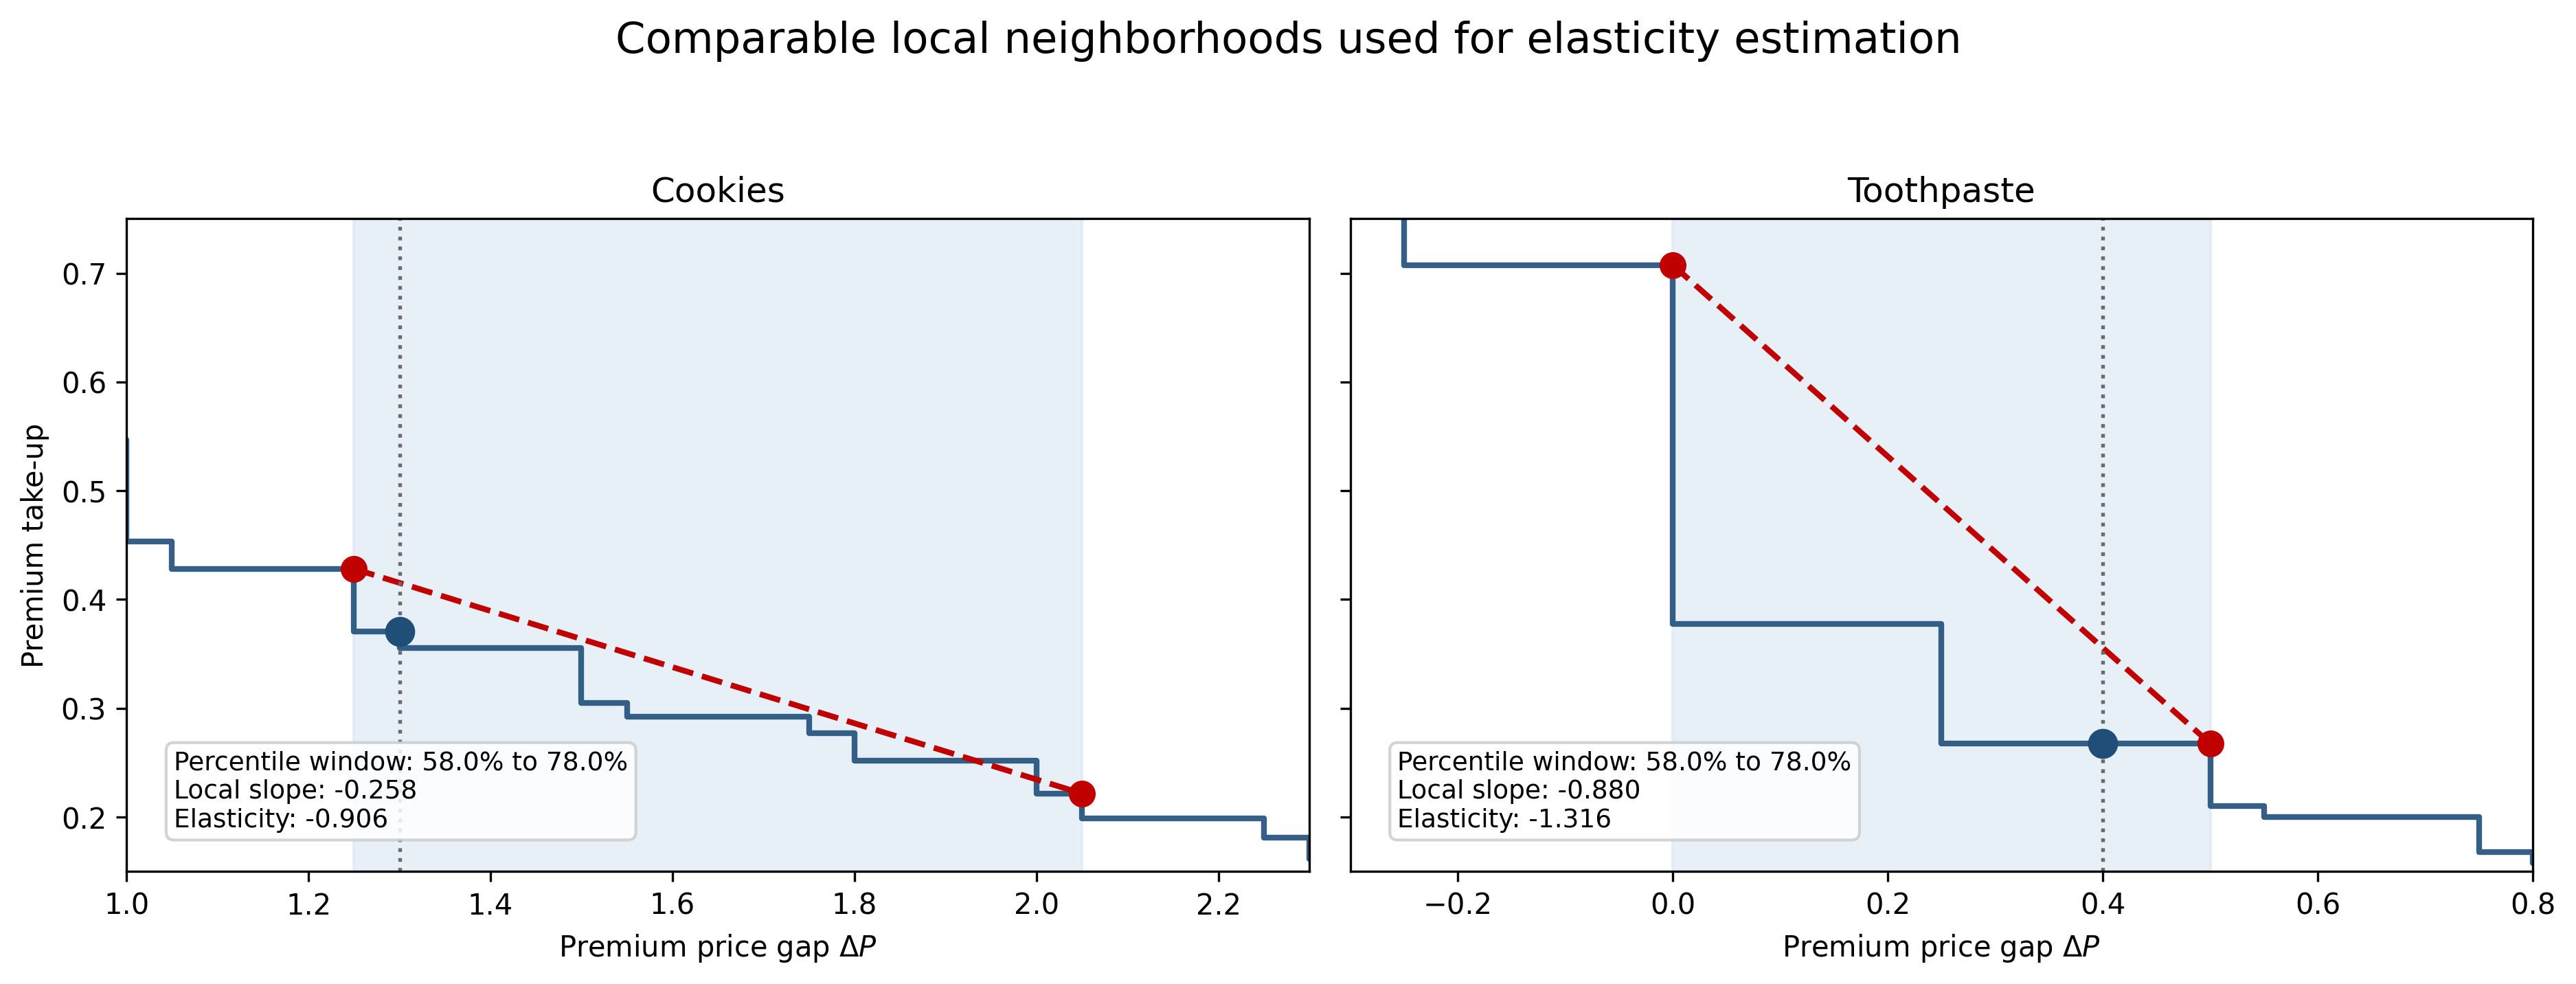
\includegraphics[width=\textwidth]{figures/wtp_within_cookies_tooth_local_elasticity.png}
  \end{center}
\end{frame}

% ============================================================
\section{Cross-condition comparison}
% ============================================================

\begin{frame}{Premium Demand: WTP vs Binary}
  \begin{columns}
    \column{0.5\textwidth}\centering Cookies\\[2pt]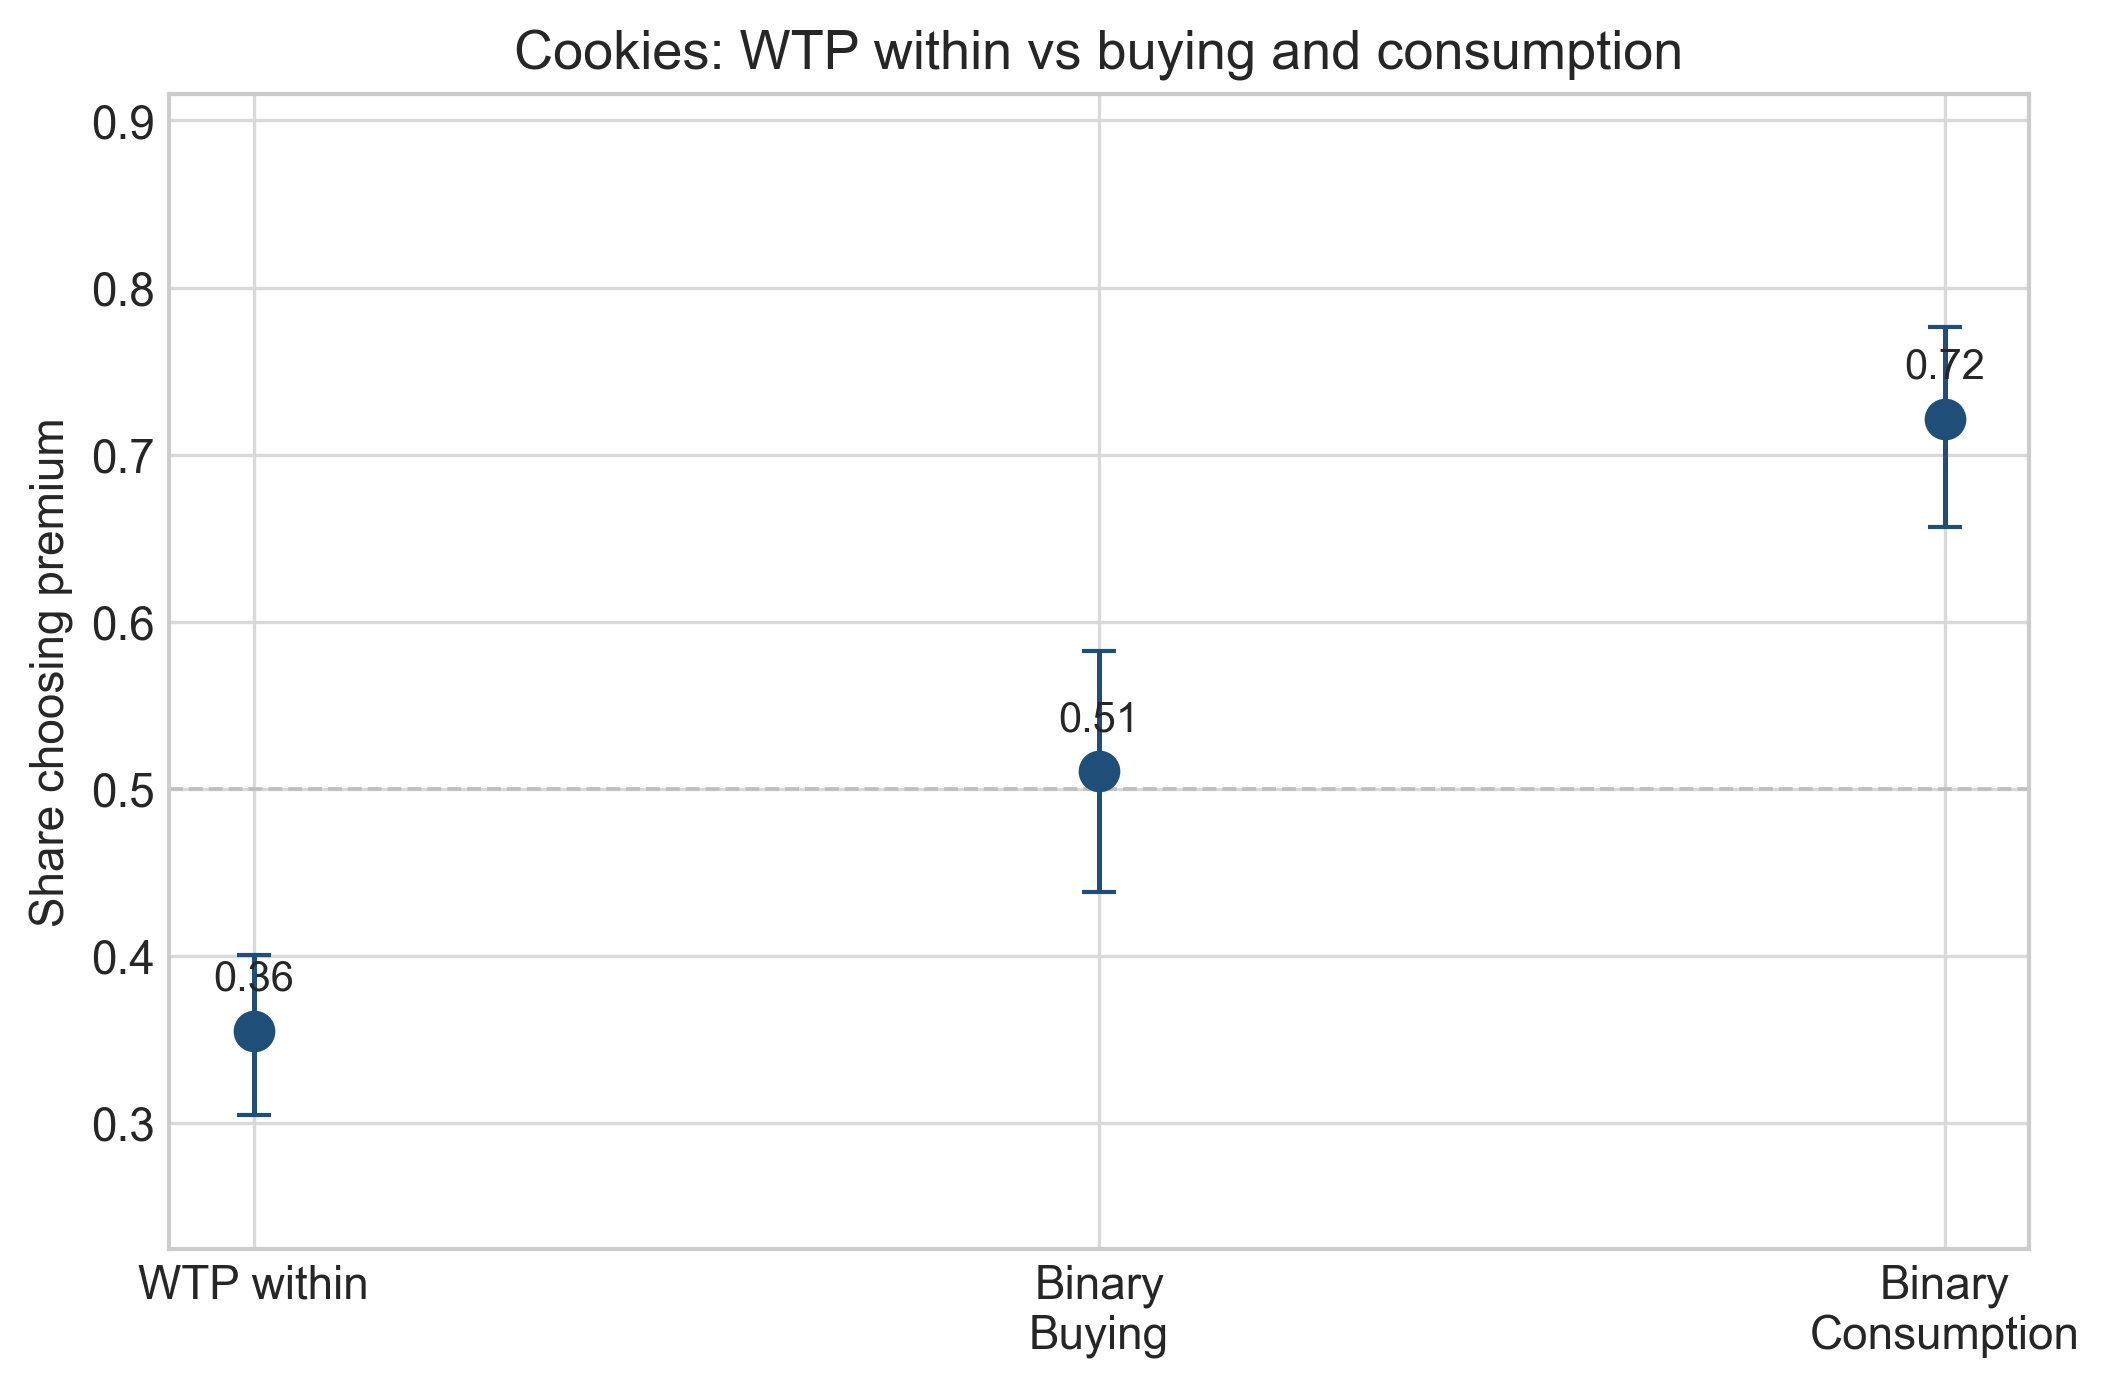
\includegraphics[width=\textwidth]{figures/cross_condition_cookies_premium_share.png}
    \column{0.5\textwidth}\centering Toothpaste\\[2pt]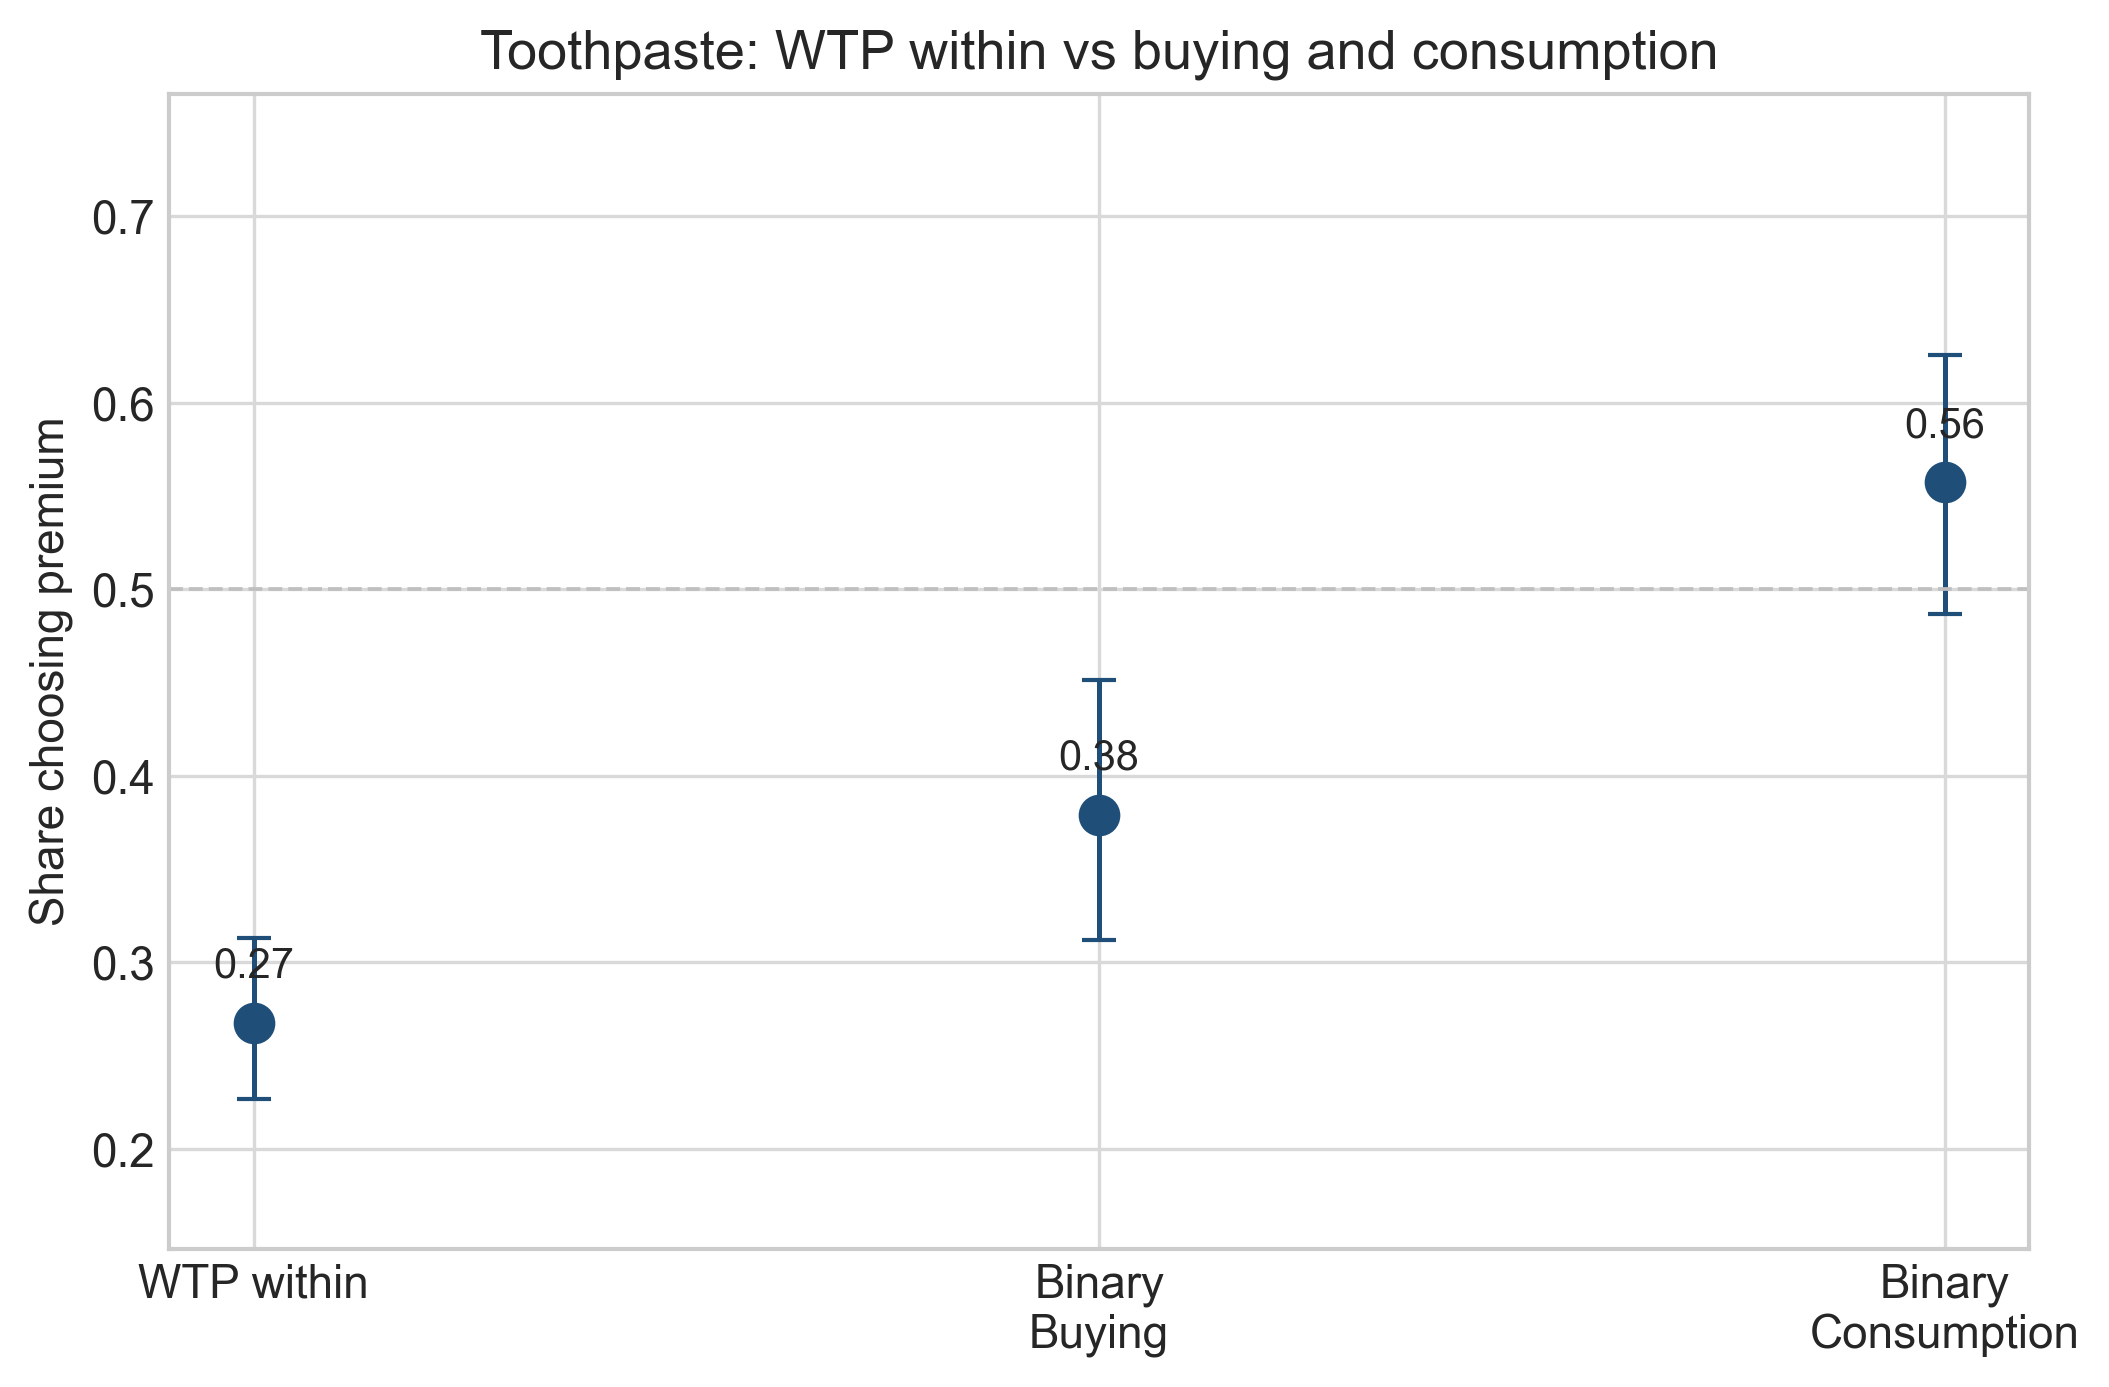
\includegraphics[width=\textwidth]{figures/cross_condition_toothpaste_premium_share.png}
  \end{columns}
\end{frame}

\begin{frame}{Attention tracks take-up across tasks}
  \hypertarget{main:cross_attention}{}

  Across all tasks, higher attention to quality attention is associated with higher premium take-up.\medskip  \hfill\hyperlink{app:cross_attention_multiple_choice}{\beamerbutton{Multiple-choice version}}

  \begin{columns}
    \column{0.5\textwidth}\centering Cookies\\[2pt]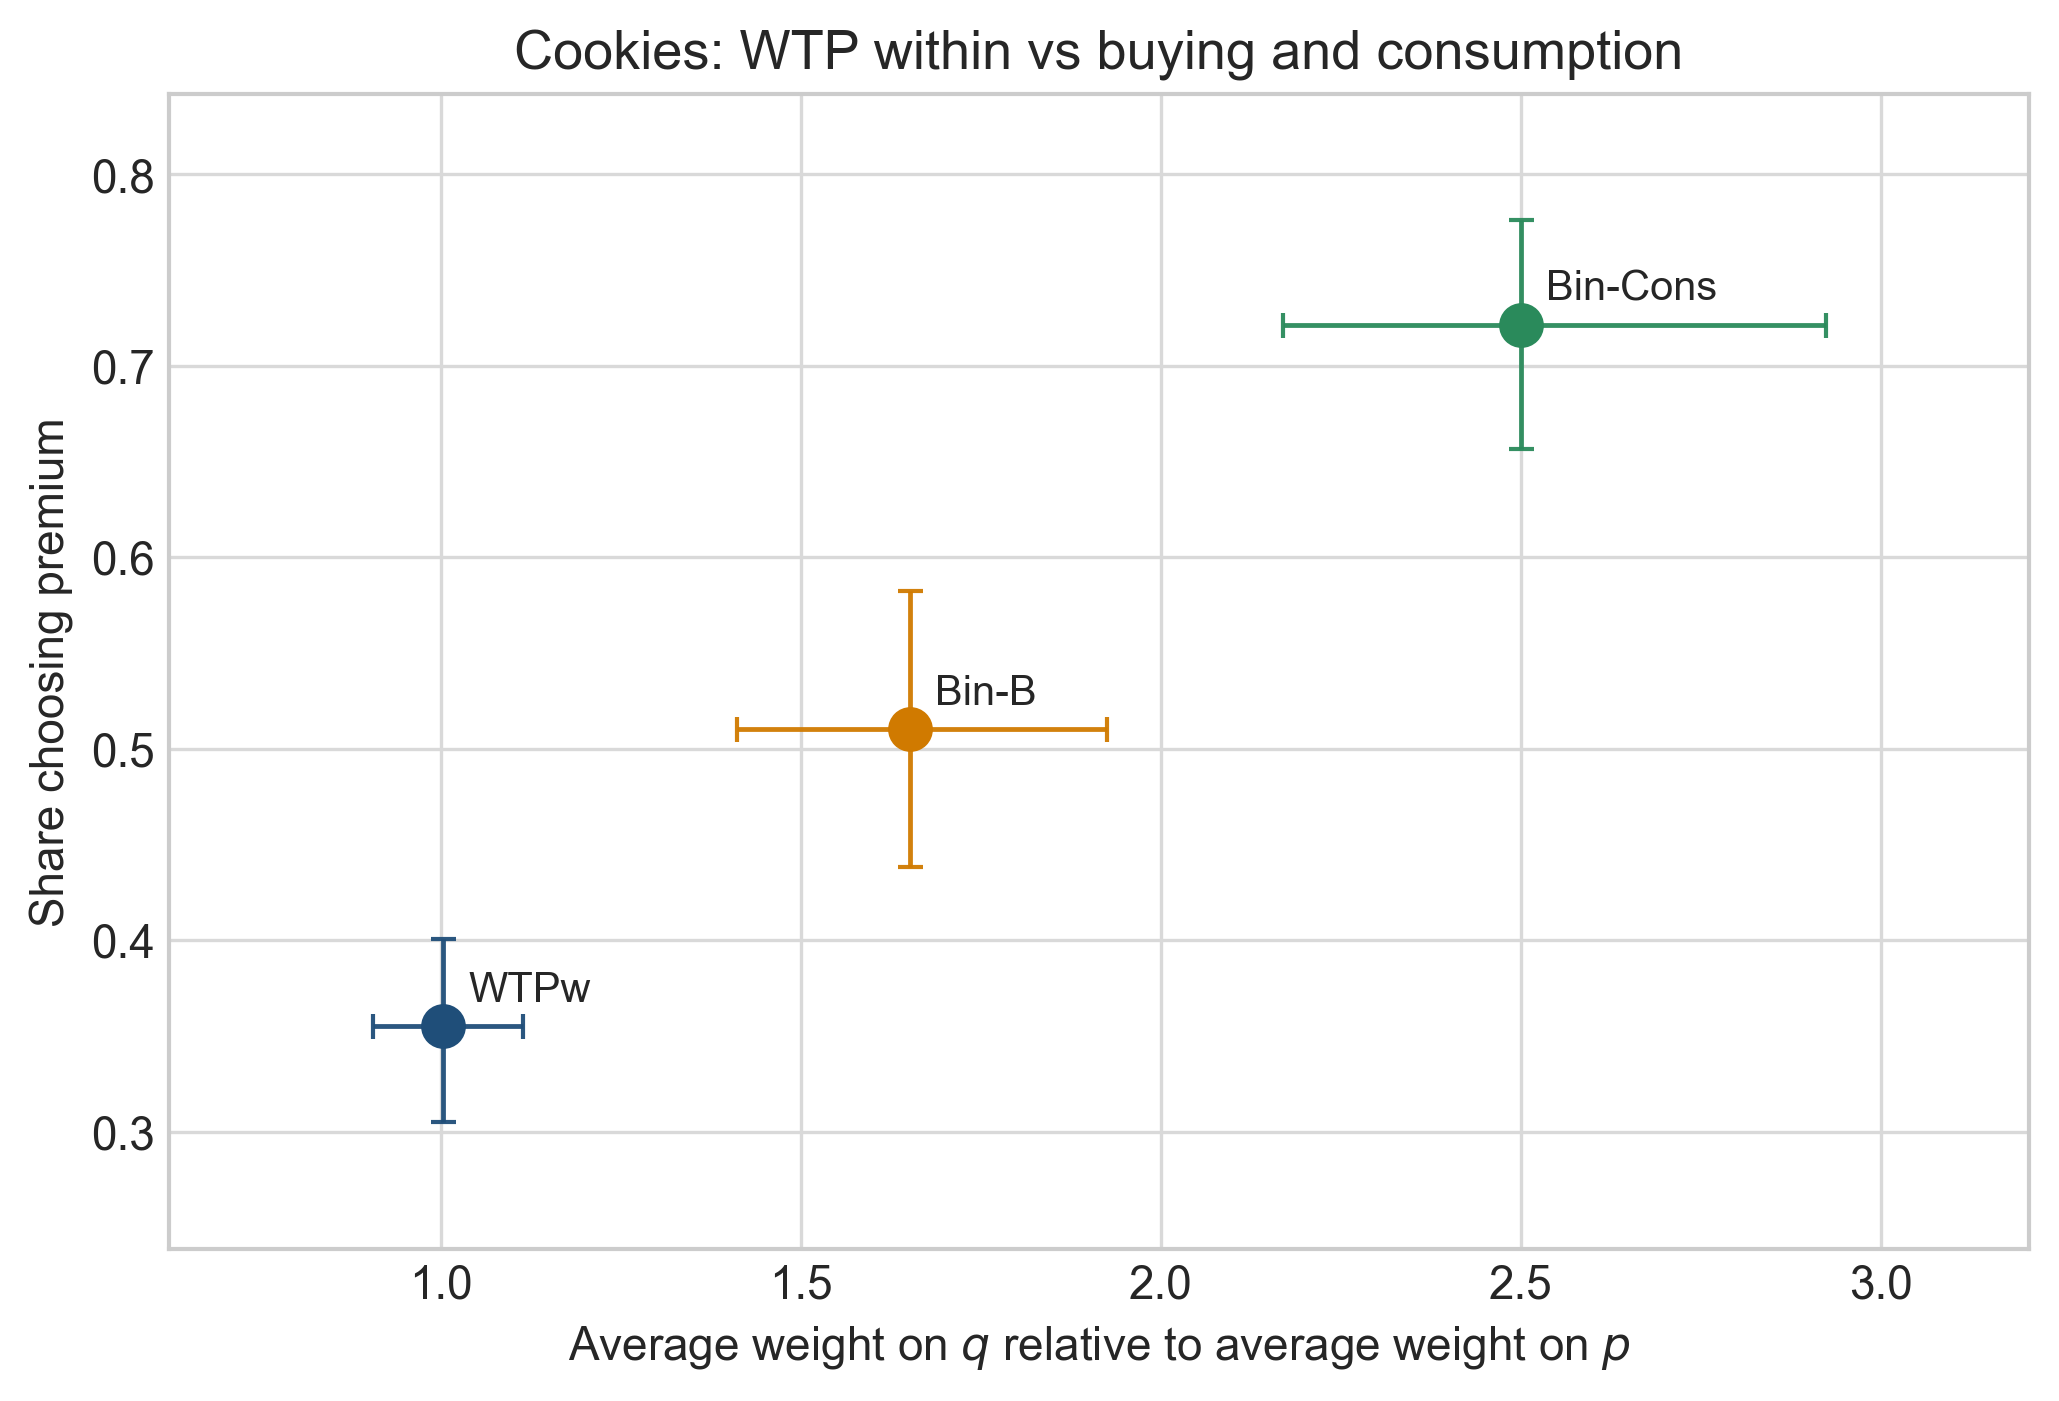
\includegraphics[width=\textwidth]{figures/cross_condition_cookies_attention_vs_premium_share.png}
    \column{0.5\textwidth}\centering Toothpaste\\[2pt]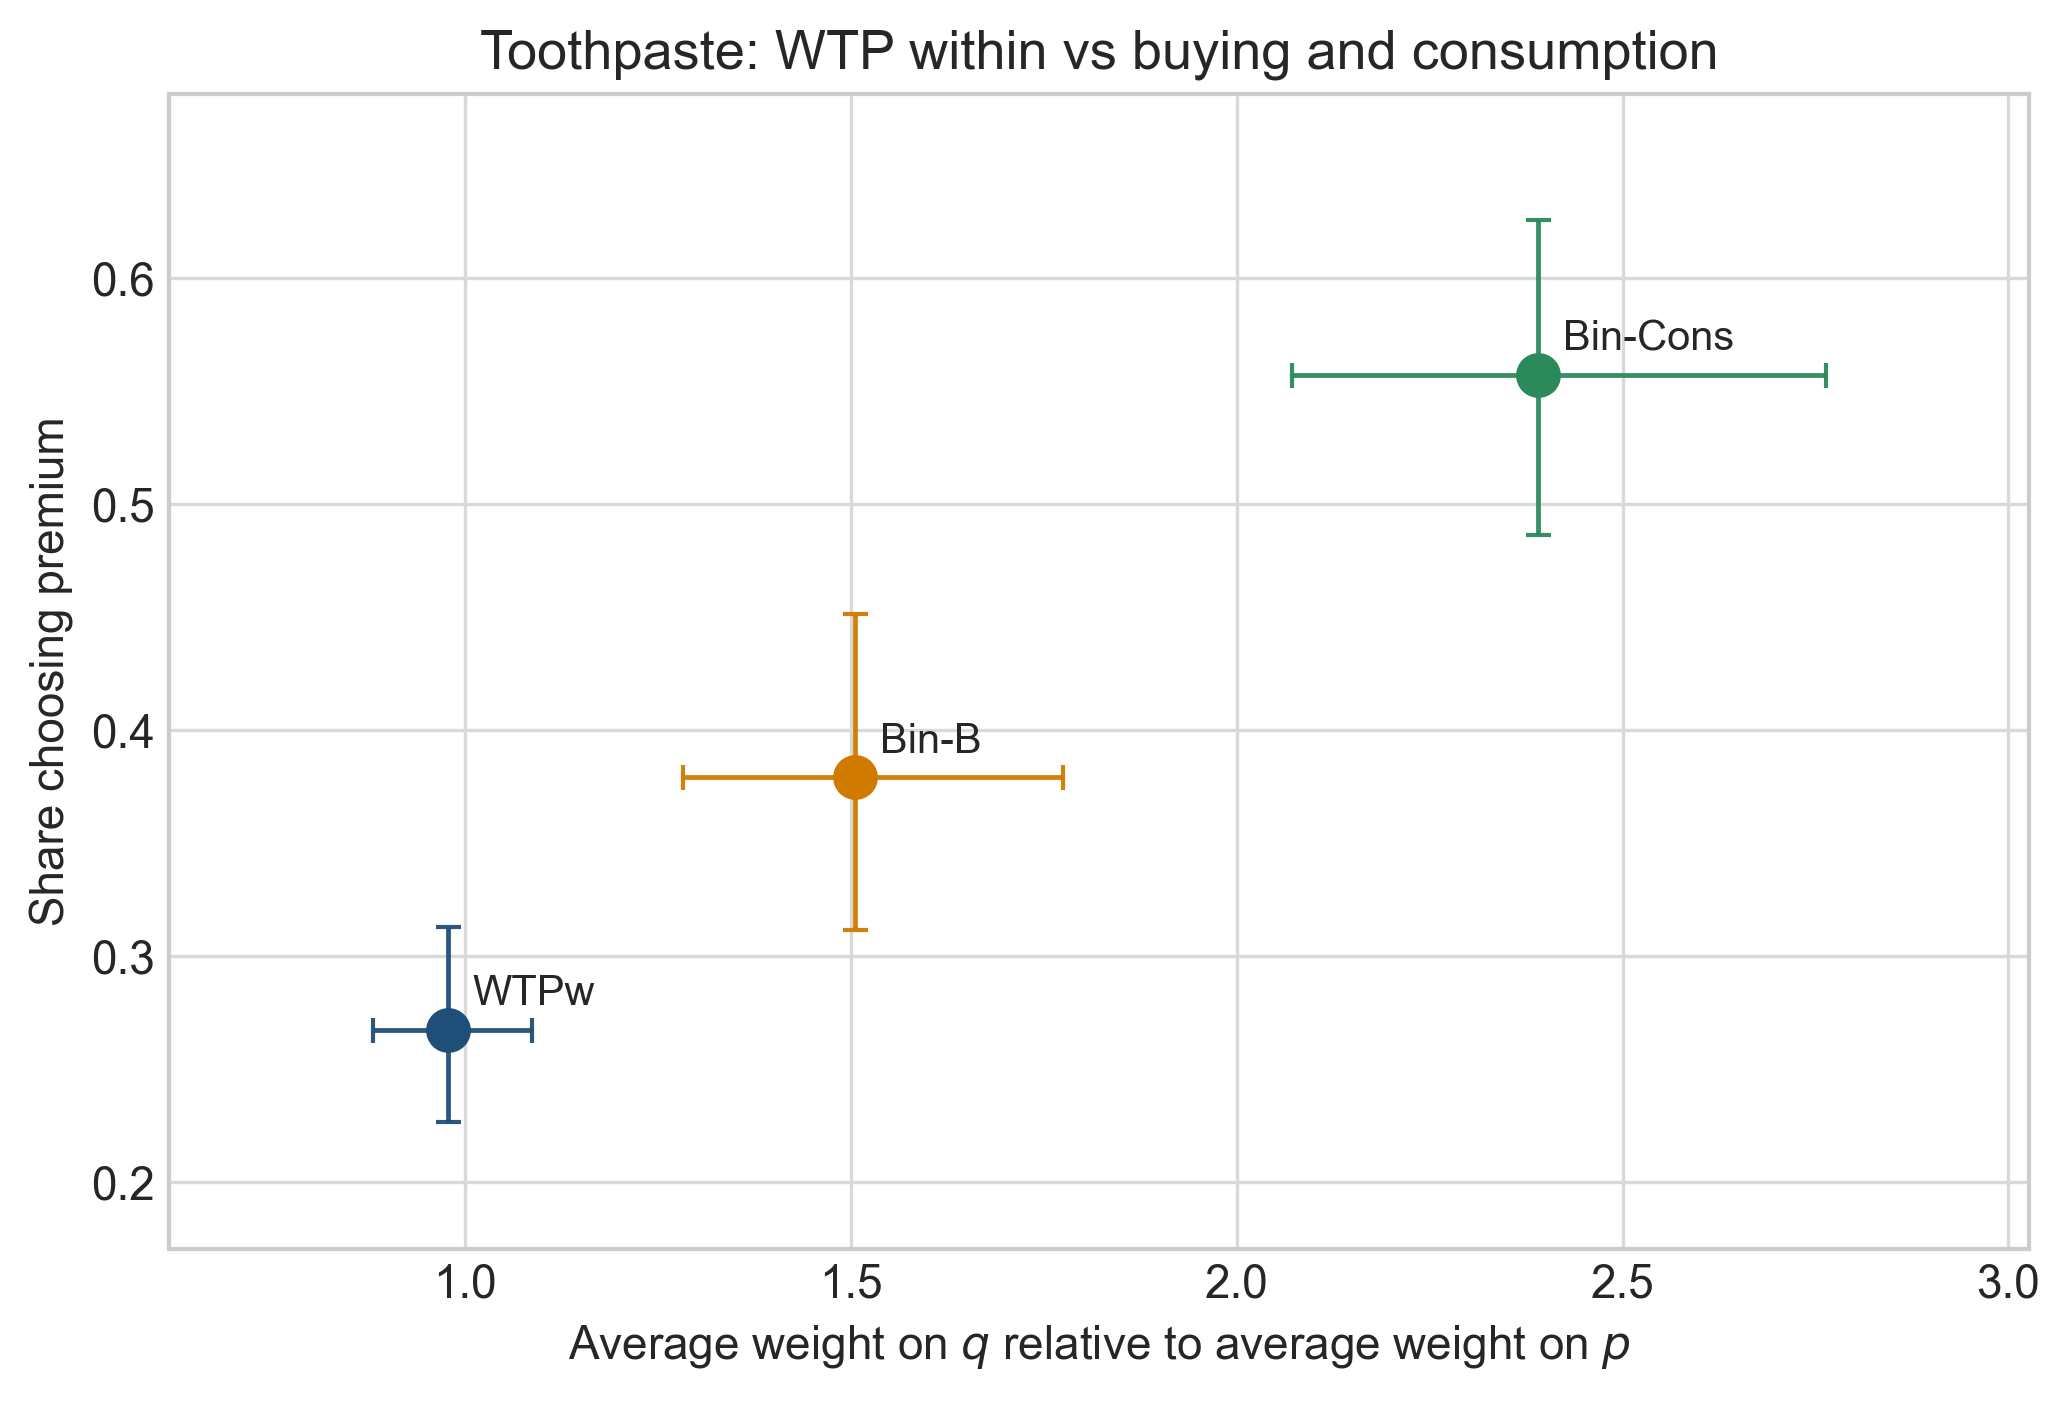
\includegraphics[width=\textwidth]{figures/cross_condition_toothpaste_attention_vs_premium_share.png}
  \end{columns}
  % \src{D3 Fig 2 (self-reported) and Fig 3 (LLM); D3 Table 4 (attention predicts take-up).}
\end{frame}


\begin{frame}{ Actual vs attention-predicted premium take-up}
\medskip
\begin{columns}[c,onlytextwidth]

\begin{column}{0.44\textwidth}
\centering
\resizebox{\linewidth}{!}{%
\renewcommand{\arraystretch}{1.12}
\begin{tabular}{@{}l r@{}}
\toprule
 & Premium take-up \\
\cmidrule(lr){2-2}
Self-reported price weight      & $-0.002^{**}$ \; \se{0.001} \\
\addlinespace[2pt]
\multicolumn{2}{@{}l}{Self-reported category (base: Price)} \\
\quad Quality                   & $\phantom{-}0.106^{*}$ \; \se{0.057} \\
\quad Both                      & $-0.008$ \; \se{0.045} \\
\addlinespace[2pt]
LLM price weight                & $-0.012^{***}$ \; \se{0.002} \\
\addlinespace[2pt]
\multicolumn{2}{@{}l}{LLM category (base: Price, Alternatives./Disutility)} \\
\quad Price (Reference Price)   & $\phantom{-}0.068$ \; \se{0.063} \\
\quad Quality                   & $\phantom{-}0.055$ \; \se{0.075} \\
\quad Both                      & $-0.036$ \; \se{0.057} \\
\addlinespace[2pt]
\multicolumn{2}{@{}l}{LLM valence (base: Price Too High)} \\
\quad Quality Too Low           & $-0.141$ \; \se{0.096} \\
\quad Price Too Low             & $-0.145^{***}$ \; \se{0.048} \\
\quad Quality Too High          & $-0.002$ \; \se{0.069} \\
\midrule
Controls (demo \& thrift)   & Yes   \\
Adjusted $R^2$                  & 0.348 \\
$N$                             & 781   \\
\bottomrule
\end{tabular}}\\[3pt]
{\tiny First stage with fine-tuned LLM. HC1 SE in parentheses.}
\end{column}

\begin{column}{0.56\textwidth}
\centering
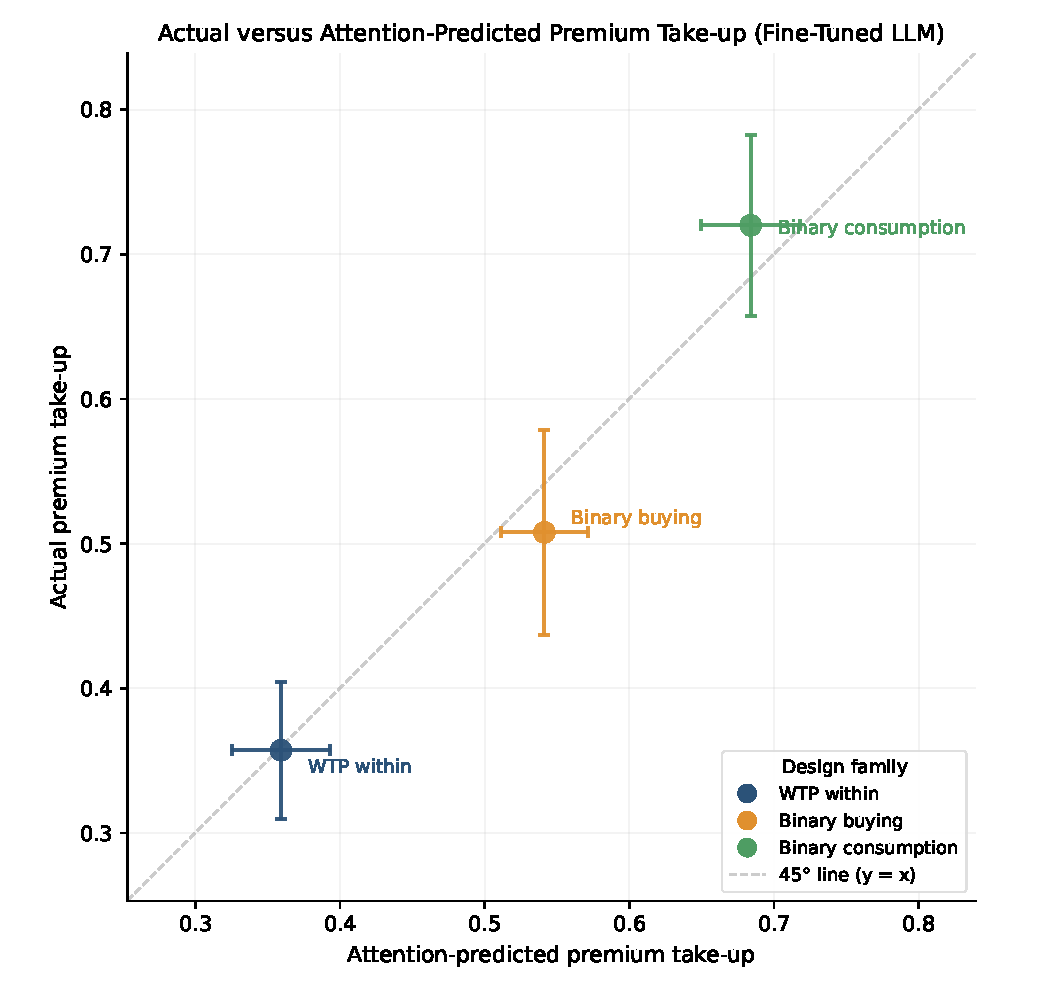
\includegraphics[width=\linewidth,trim=0 0 0 22pt,clip]{figures/fig_takeup_actual_vs_predicted.pdf}
\end{column}

\end{columns}

\vspace{1.4em}
{\scriptsize
\setlength{\abovedisplayskip}{0pt}\setlength{\belowdisplayskip}{0pt}
OLS of individual take-up on attention $A_i$ and controls $X_i$: $Y_i = f(A_i, X_i) + \varepsilon_i$, with $A_i = (\omega_{p,i}^{\mathrm{SR}},\,\omega_{p,i}^{\mathrm{LLM}},\, R_i^{\mathrm{SR}},\, R_i^{\mathrm{LLM}},\, V_i^{\mathrm{LLM}})$. Attention-only prediction: $\widehat{Y}_i = \widehat{f}(A_i,\, \overline{X})$.
\par}

\end{frame}
\begin{frame}{Demand curve and elasticity}
  The shift form WTP to Binary is equivalent to large cuts in the Premium Price gap.
  \begin{center}
    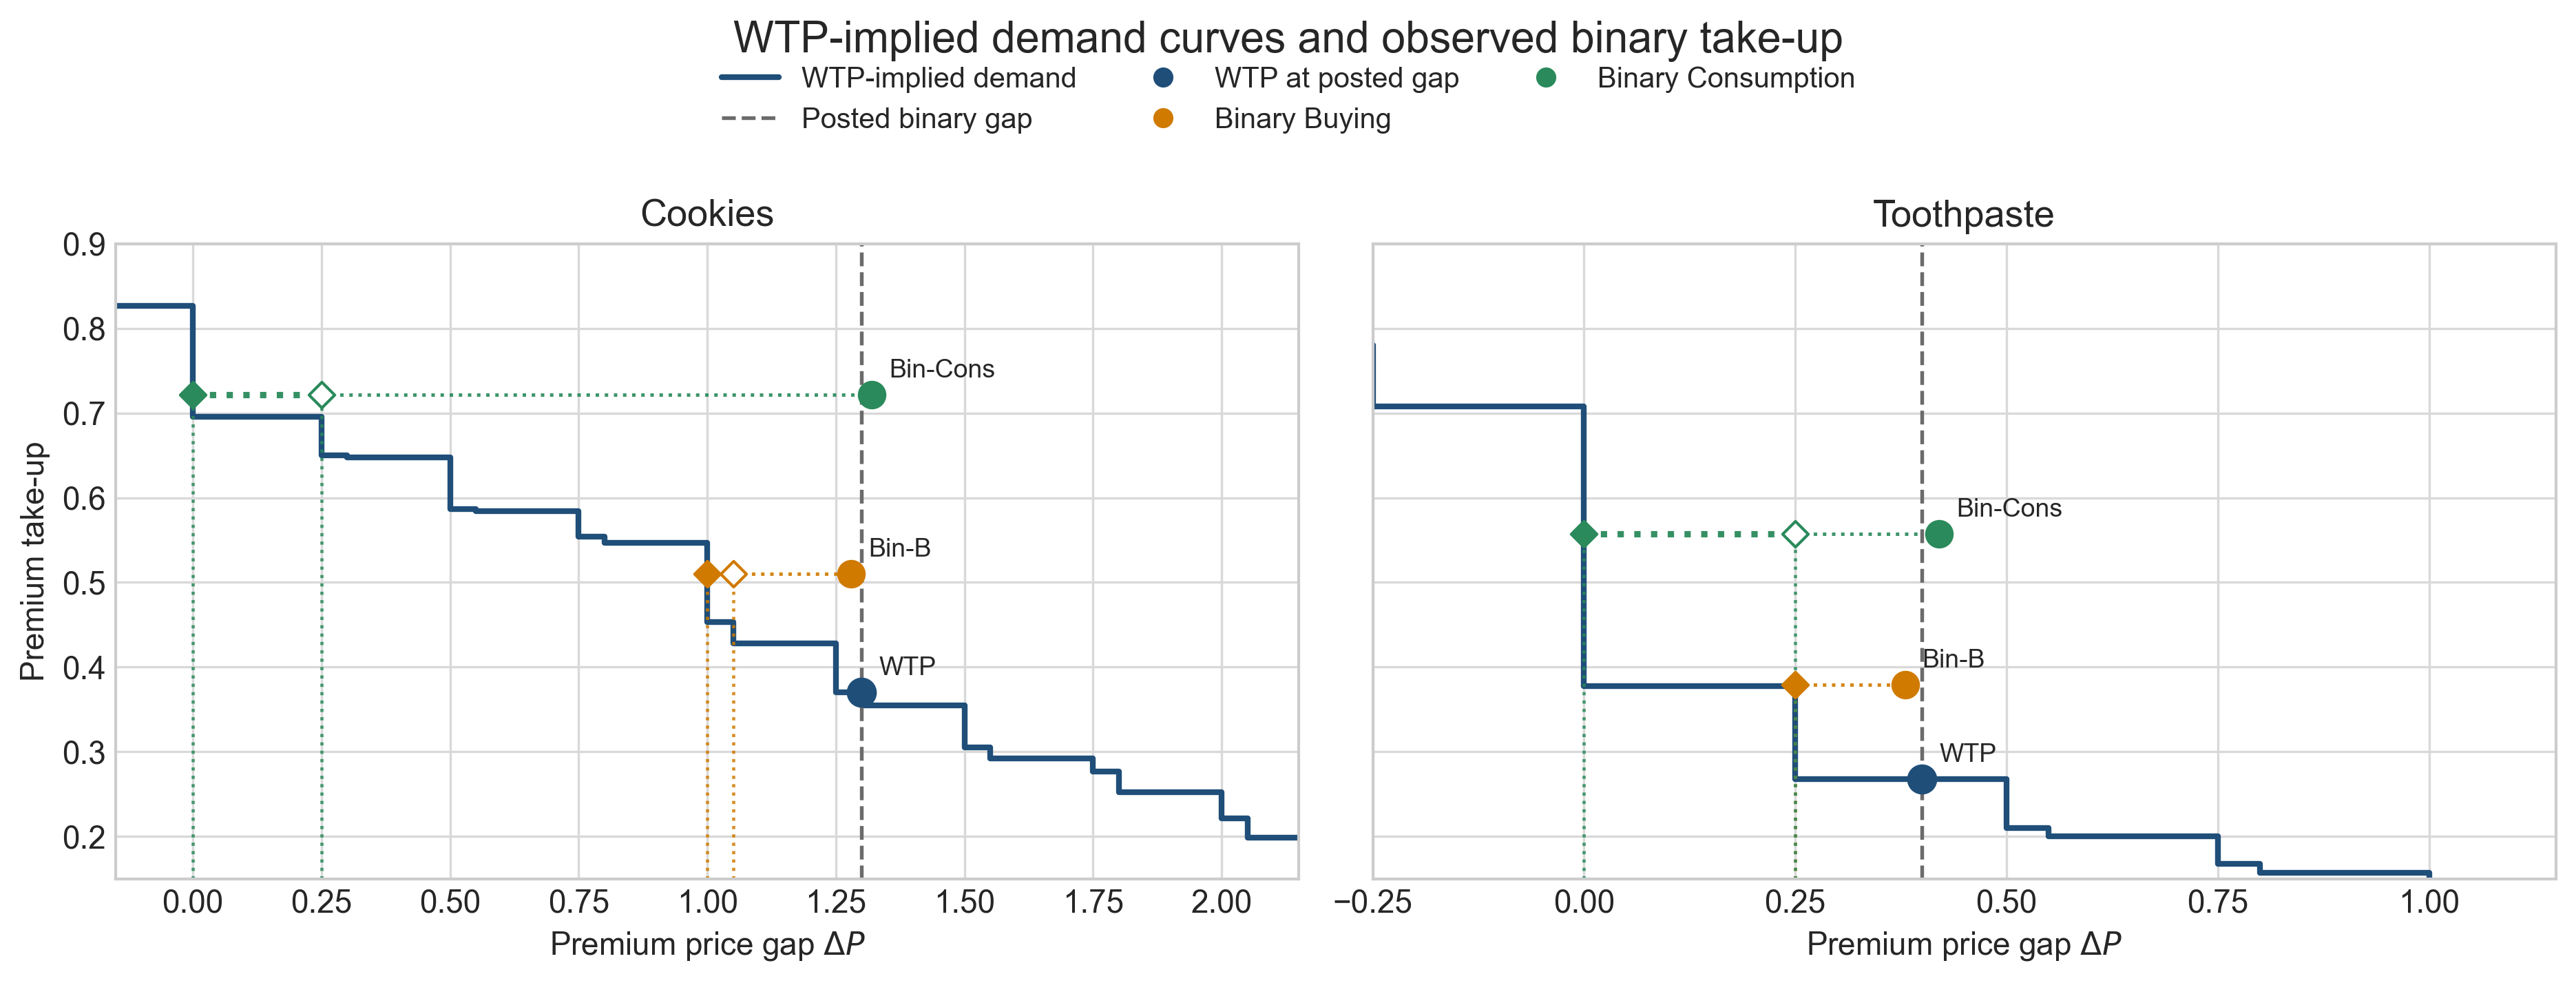
\includegraphics[width=\textwidth]{figures/cross_condition_cookies_tooth_wtp_demand_curves.png}
  \end{center}
\end{frame}

\begin{frame}{Implied price gap by good and condition}
  \begin{center}
    \scriptsize
    \begin{tabular}{llccc}
\toprule
Product & Condition & Binary share & WTP share & Implied gap \\
\midrule
Cookies & Buying & 0.510 & 0.370 & 1.00 to 1.05 \\
 & Consumption & 0.721 & 0.370 & 0.00 to 0.25 \\
\midrule
Toothpaste & Buying & 0.379 & 0.268 & 0.25 \\
 & Consumption & 0.557 & 0.268 & 0.00 to 0.25 \\
\bottomrule
\end{tabular}

  \end{center}
\end{frame}

\section{WTA}
% ============================================================

\begin{frame}{WTA strong: task structure}
  \begin{itemize}
    \item Participants face a multiple-price-list task for the premium brand only.
    \item Instead of indicating willingness to buy, they indicate whether they would keep the premium good or give it up for a stated amount.
    \item The switching point in that list gives the participant's WTA strong valuation for the premium product.
    \item In the current pilot, this elicitation exists for cookies only; toothpaste has not yet been run.
  \end{itemize}
\end{frame}

\begin{frame}{WTA strong: participant flow}
  \begin{itemize}
    \item This is a premium-only task: there is no parallel MPL for the regular brand in the same protocol.
    \item The design is between-subjects relative to WTP: one set of participants completes WTP, another completes WTA strong.
    \item The direct comparison is therefore between premium valuations elicited under buying in WTP and under giving-up/keeping in WTA strong.
  \end{itemize}
\end{frame}

\begin{frame}{The observed gap}
  Selling (WTA strong) values the premium good above buying (WTP).
  \begin{center}
    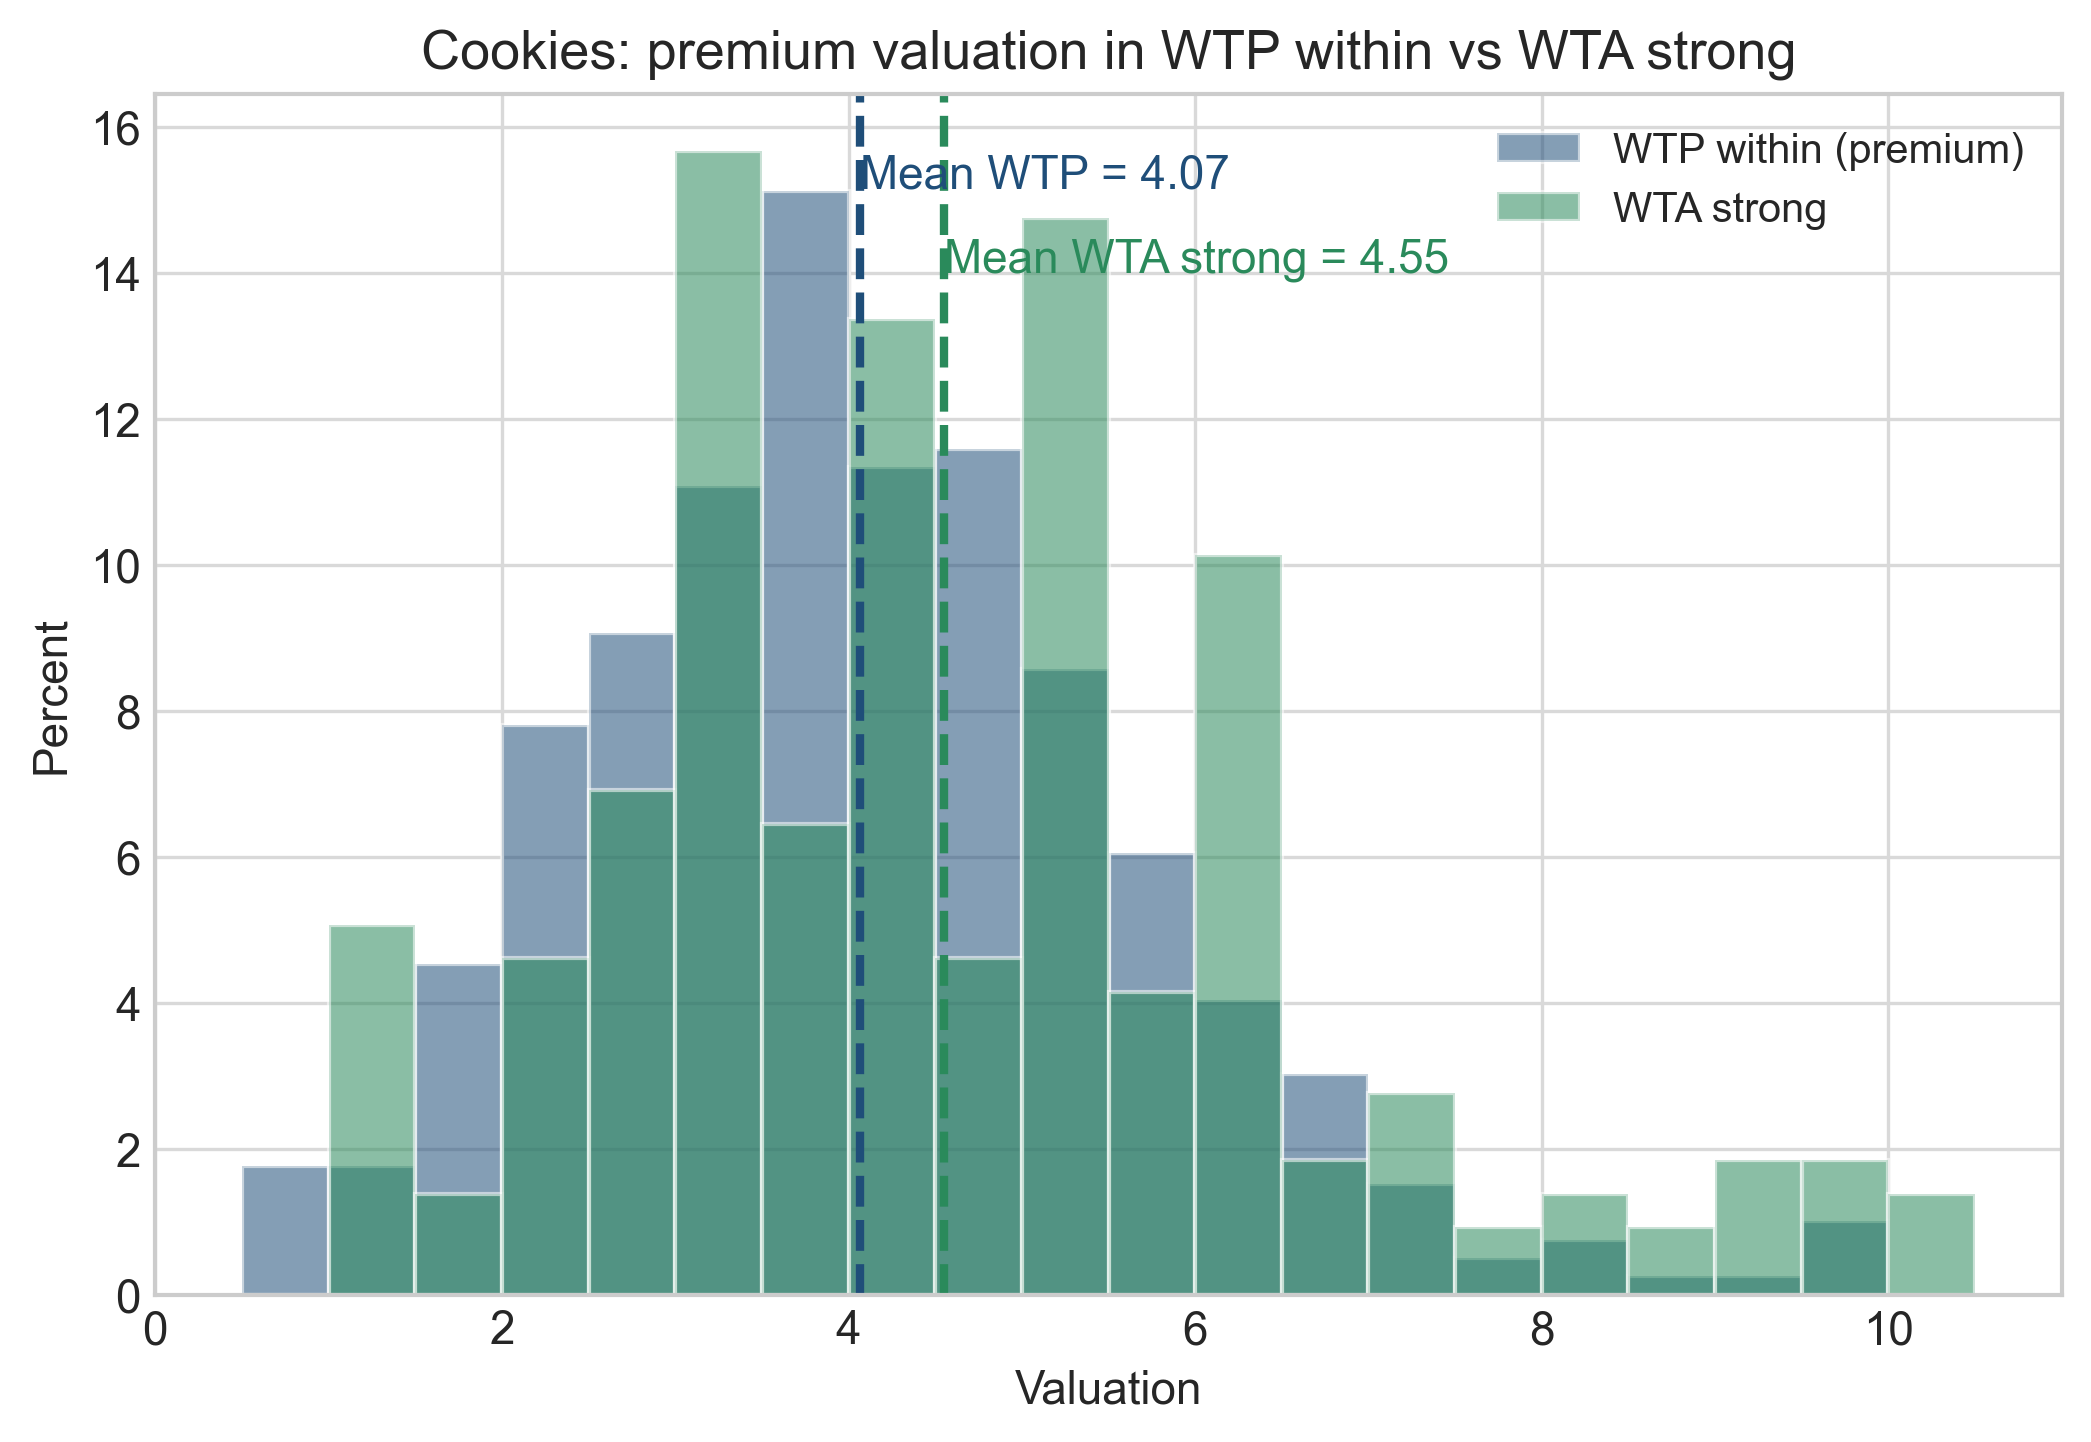
\includegraphics[width=0.76\textwidth]{figures/wta_strong_cookies_price_distribution.png}
  \end{center}
  % \src{D1 Fig 5 / Table 5 (cookies): 4.07/4.28/4.55; strong gap $+0.48$, p$=0.002$. Toothpaste ?}
\end{frame}

\begin{frame}{Attention and the gap}
  \hypertarget{main:wta_attention}{}
  \hfill\hyperlink{app:wta_attention_multiple_choice}{\beamerbutton{Multiple-choice version}}
  \medskip
  \begin{center}
    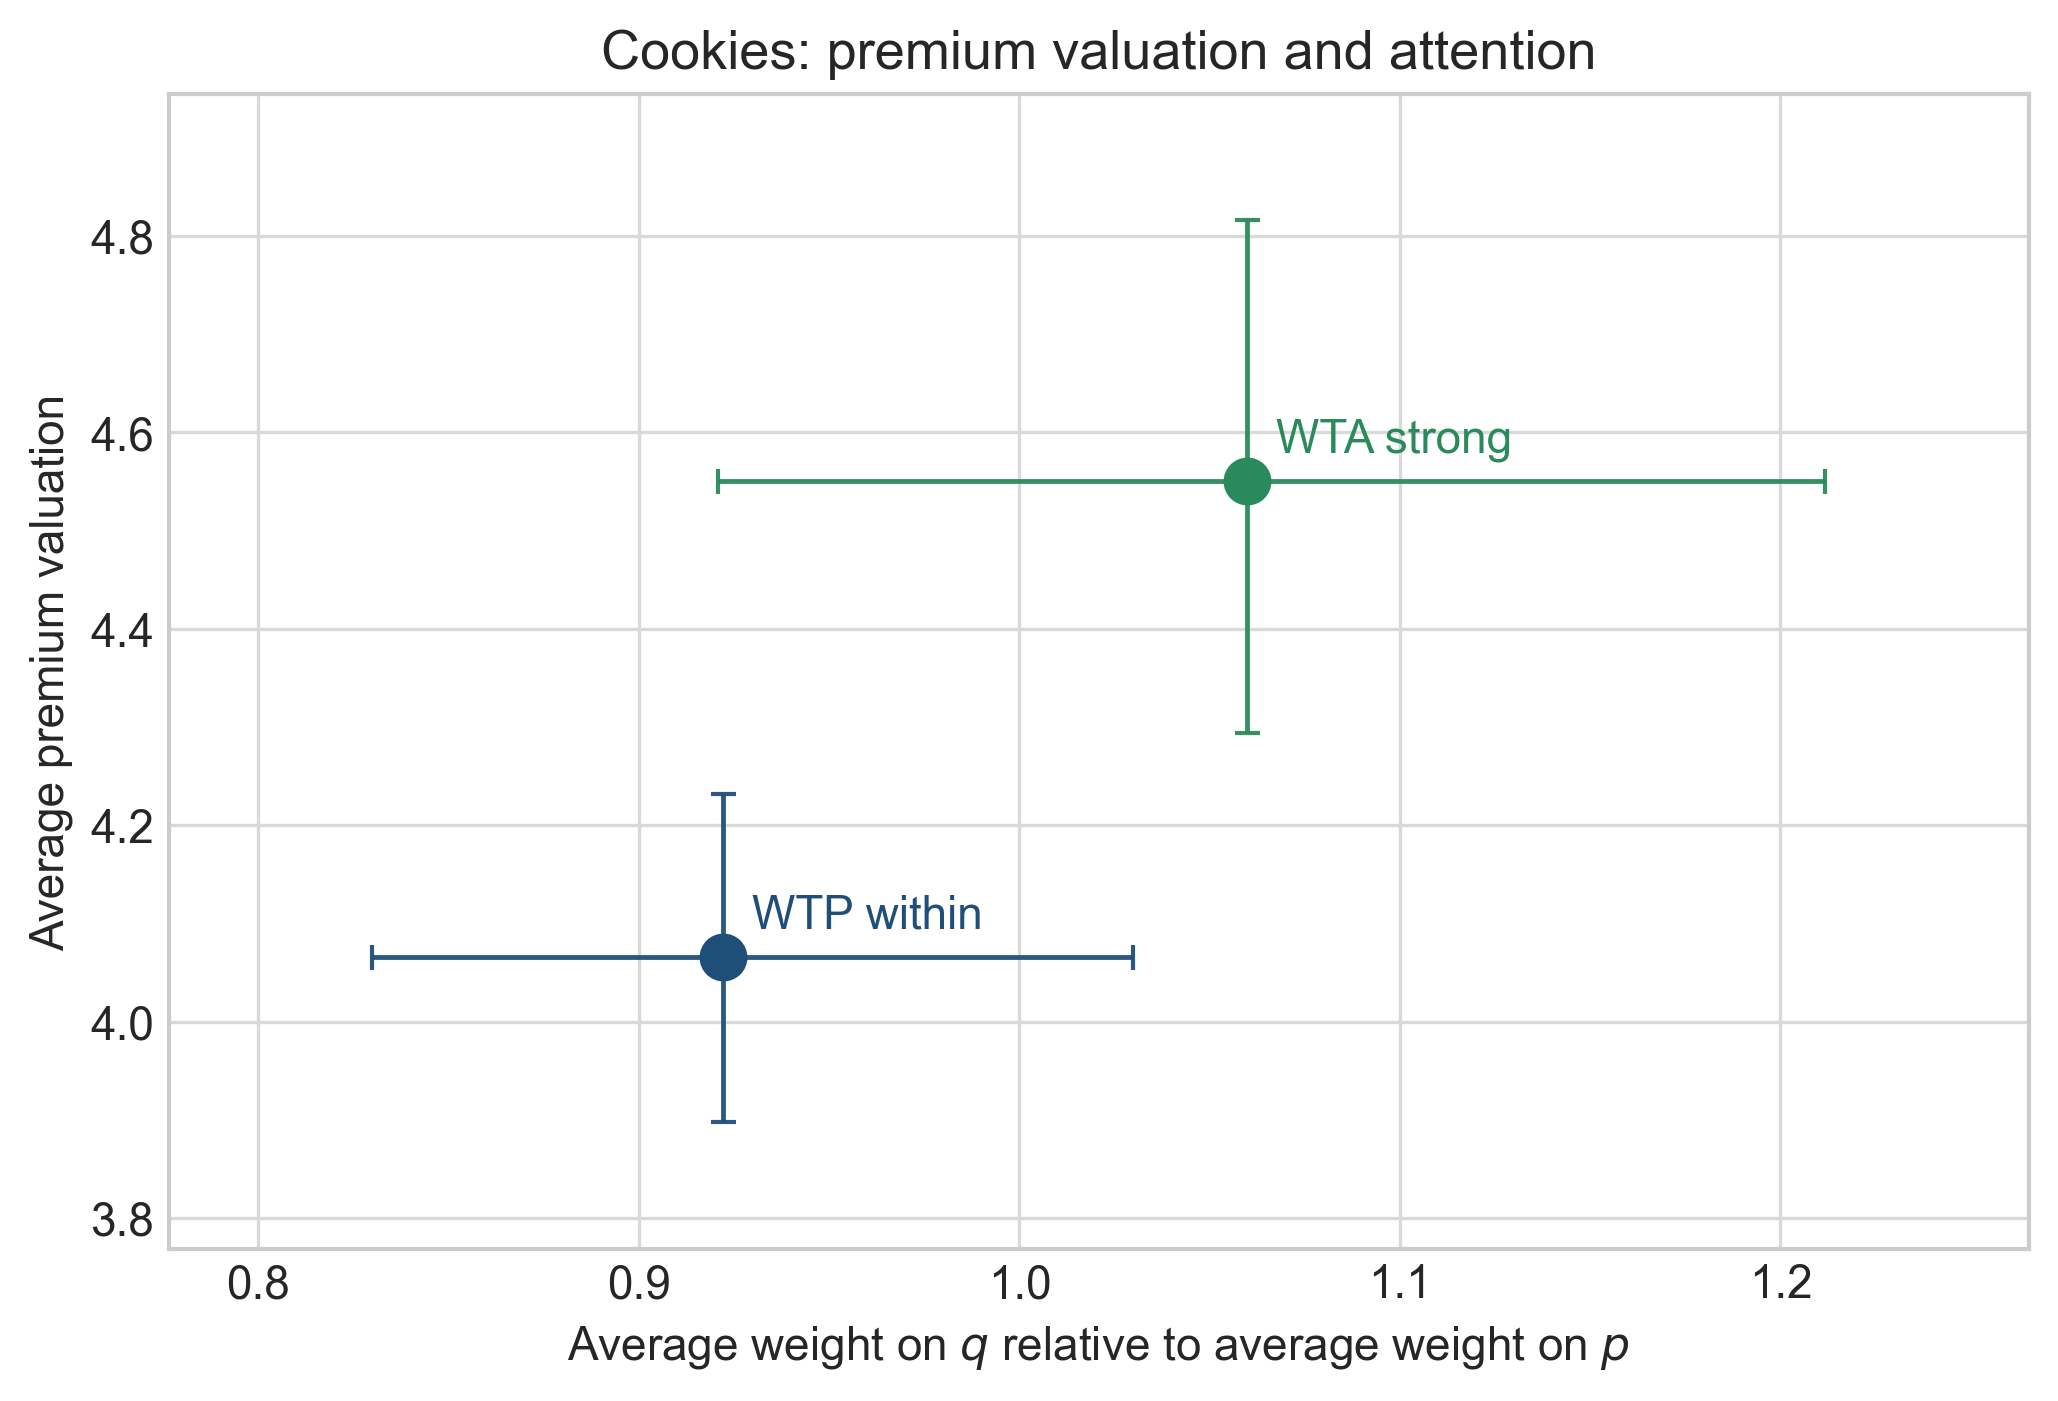
\includegraphics[width=0.75\textwidth]{figures/wta_strong_cookies_ratio_vs_price.png}
  \end{center}
\end{frame}




\begin{frame}{Actual vs attention-predicted premium valuation}
\medskip
\begin{columns}[c,onlytextwidth]

\begin{column}{0.44\textwidth}
\centering
\resizebox{\linewidth}{!}{%
\renewcommand{\arraystretch}{1.12}
\begin{tabular}{@{}l r@{}}
\toprule
 & Premium valuation (\$) \\
\cmidrule(lr){2-2}
Self-reported price weight      & $-0.015^{***}$ \; \se{0.004} \\
\addlinespace[2pt]
\multicolumn{2}{@{}l}{Self-reported category (base: Price)} \\
\quad Quality                   & $-0.177$ \; \se{0.251} \\
\quad Both                      & $\phantom{-}0.067$ \; \se{0.165} \\
\addlinespace[2pt]
LLM price weight                & $-0.033^{***}$ \; \se{0.009} \\
\addlinespace[2pt]
\multicolumn{2}{@{}l}{LLM category (base: Price, Alternatives./Disutility)} \\
\quad Price (Reference Price)   & $\phantom{-}0.190$ \; \se{0.230} \\
\quad Quality                   & $-0.558$ \; \se{0.353} \\
\quad Both                      & $-0.306$ \; \se{0.194} \\
\addlinespace[2pt]
\multicolumn{2}{@{}l}{LLM valence (base: Price Too High)} \\
\quad Quality Too Low           & $-1.216^{***}$ \; \se{0.430} \\
\quad Price Too Low             & $\phantom{-}0.172$ \; \se{0.202} \\
\quad Quality Too High          & $\phantom{-}0.549^{**}$ \; \se{0.271} \\
\midrule
Controls (demo \& thrift)  & Yes   \\
Adjusted $R^2$                  & 0.195 \\
$N$                             & 595   \\
\bottomrule
\end{tabular}}\\[3pt]
{\tiny First stage with fine-tuned LLM. HC1 SE in parentheses.}
\end{column}

\begin{column}{0.56\textwidth}
\centering
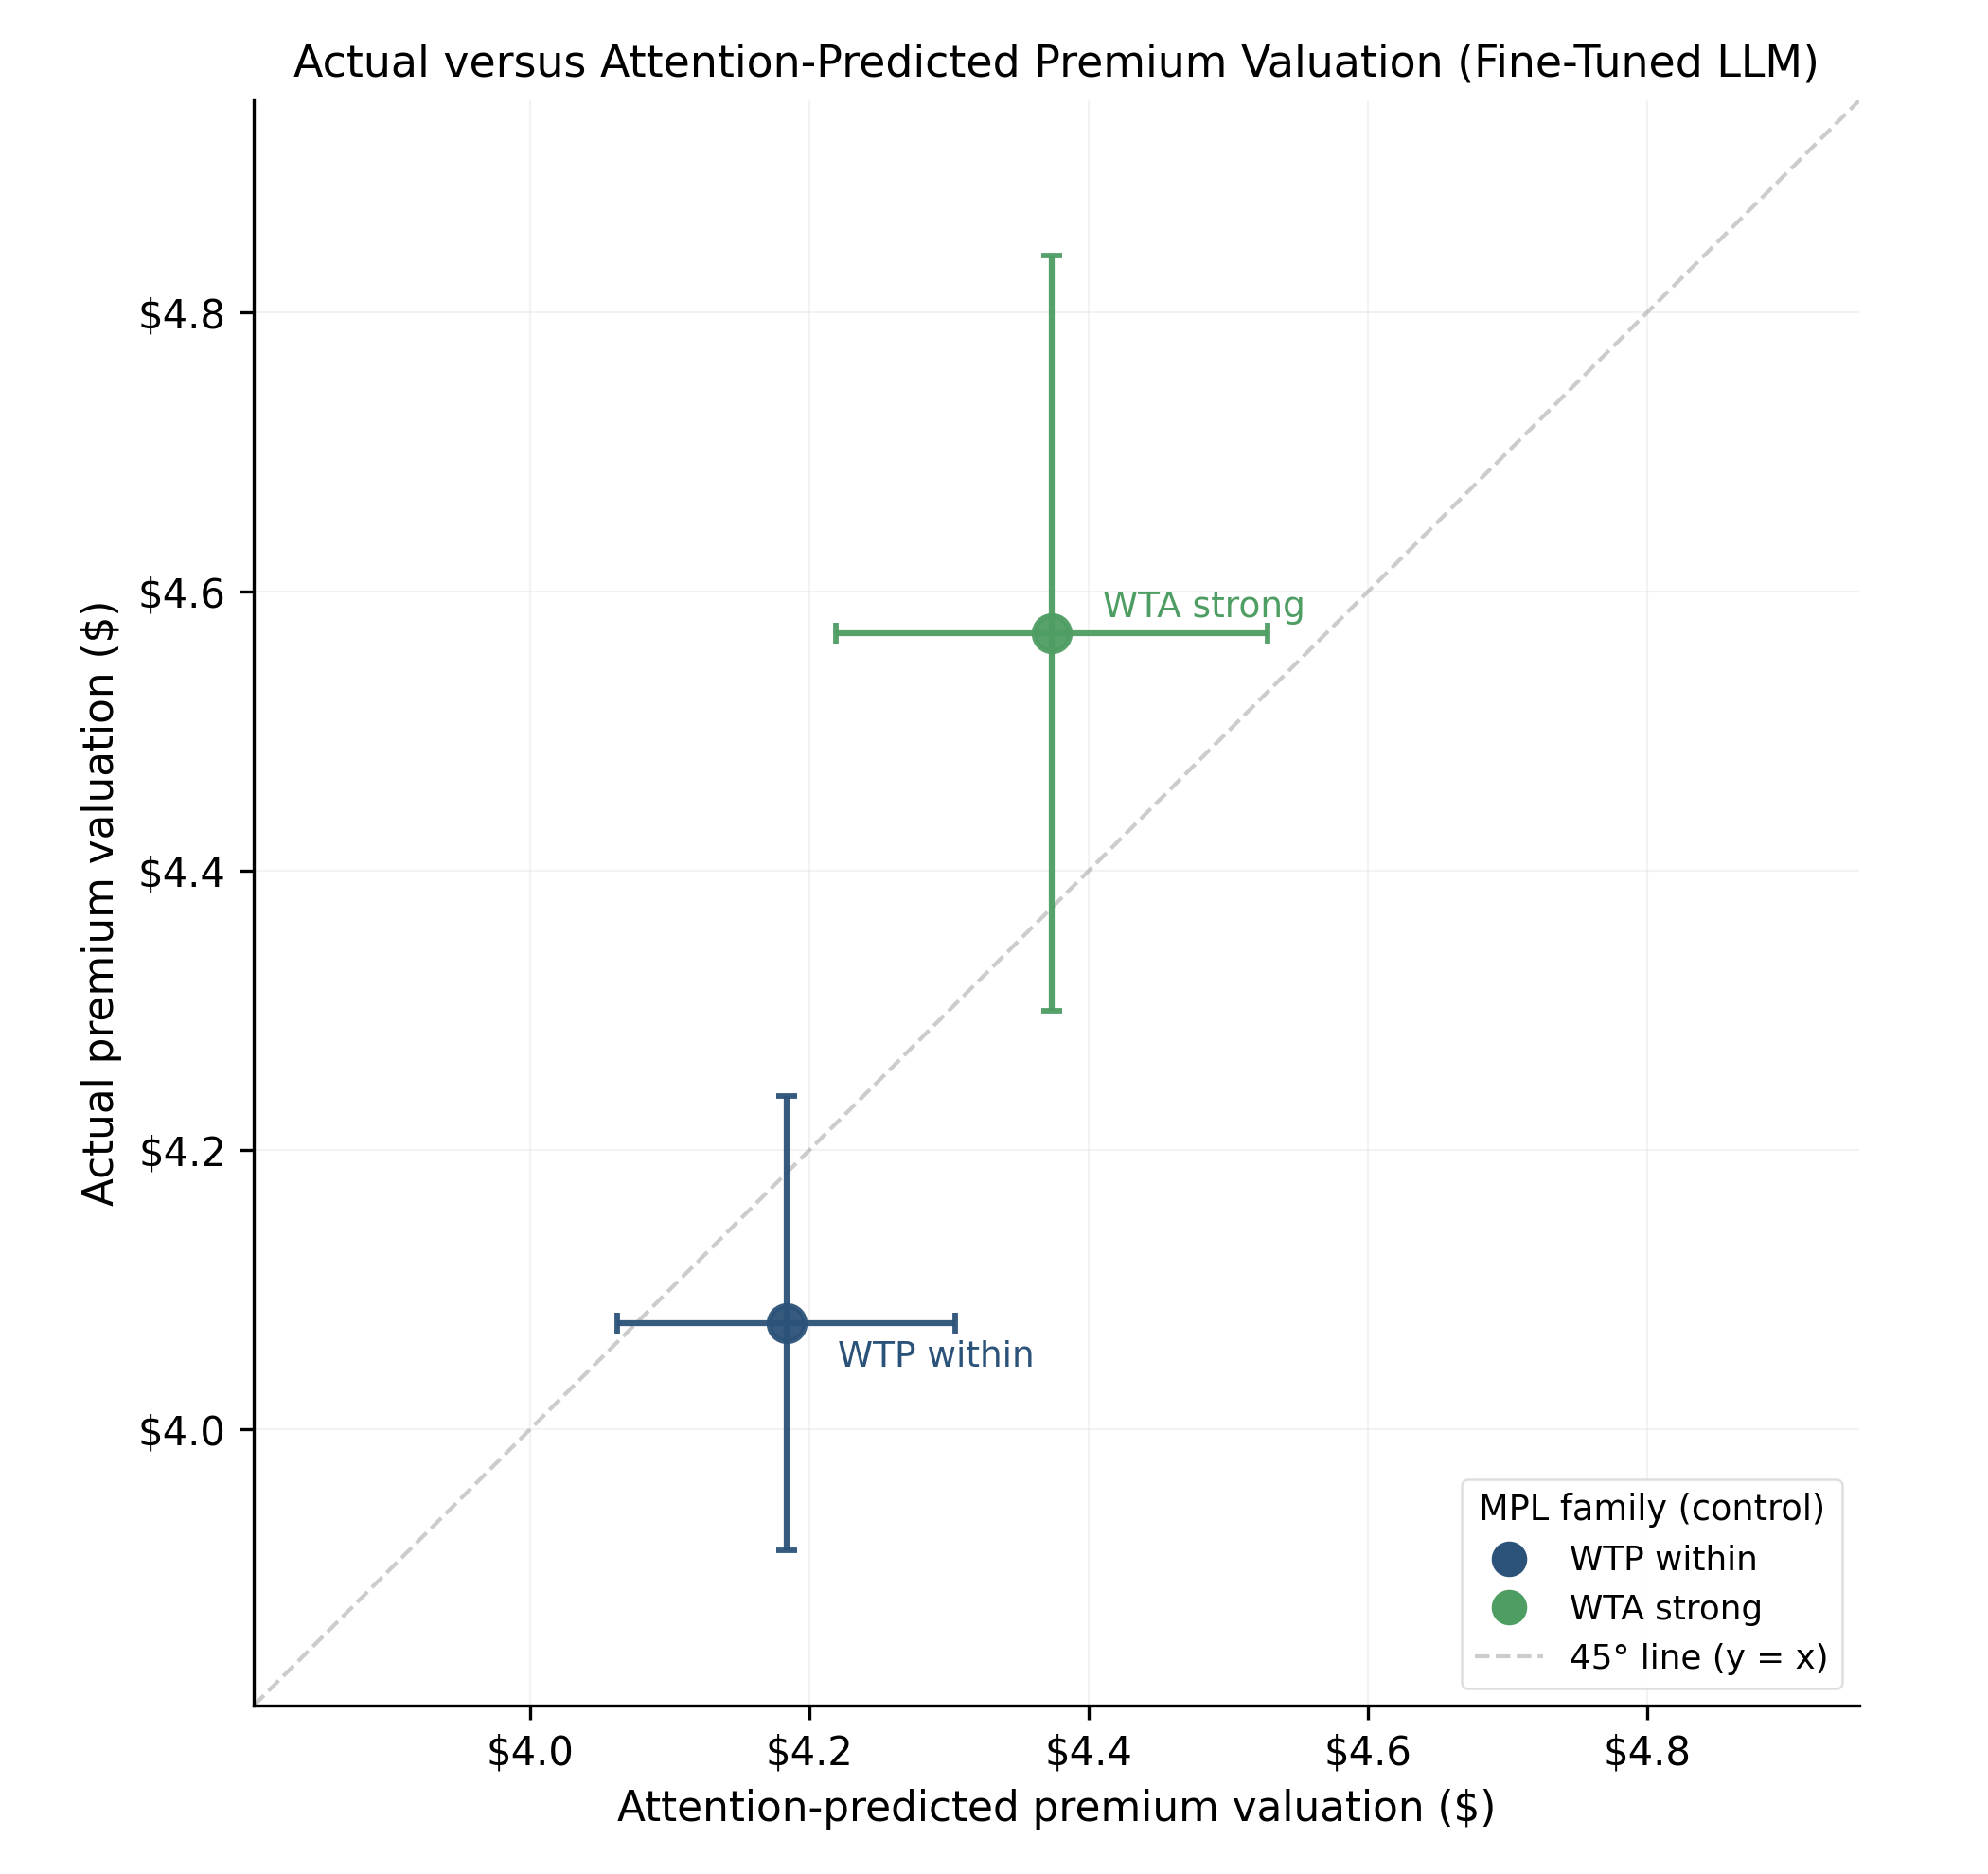
\includegraphics[width=\linewidth,trim=0 0 0 22pt,clip]{figures/fig_valuation_actual_vs_predicted.png}
\end{column}

\end{columns}

\vspace{1.4em}
{\scriptsize
\setlength{\abovedisplayskip}{0pt}\setlength{\belowdisplayskip}{0pt}
OLS of individual take-up on attention $A_i$ and controls $X_i$: $Y_i = f(A_i, X_i) + \varepsilon_i$, with $A_i = (\omega_{p,i}^{\mathrm{SR}},\,\omega_{p,i}^{\mathrm{LLM}},\, R_i^{\mathrm{SR}},\, R_i^{\mathrm{LLM}},\, V_i^{\mathrm{LLM}})$. Attention-only prediction: $\widehat{Y}_i = \widehat{f}(A_i,\, \overline{X})$.
\par}

\end{frame}



\begin{frame}{Combining self-reported and LLM}
  \hypertarget{main:wta_combined}{}
  \hfill\hyperlink{app:wta_gap_predicted}{\beamerbutton{Predicted gap slide}}
  \medskip
  Decomposition is where text adds value. (reference price vs opportunity cost).
  \begin{center}
    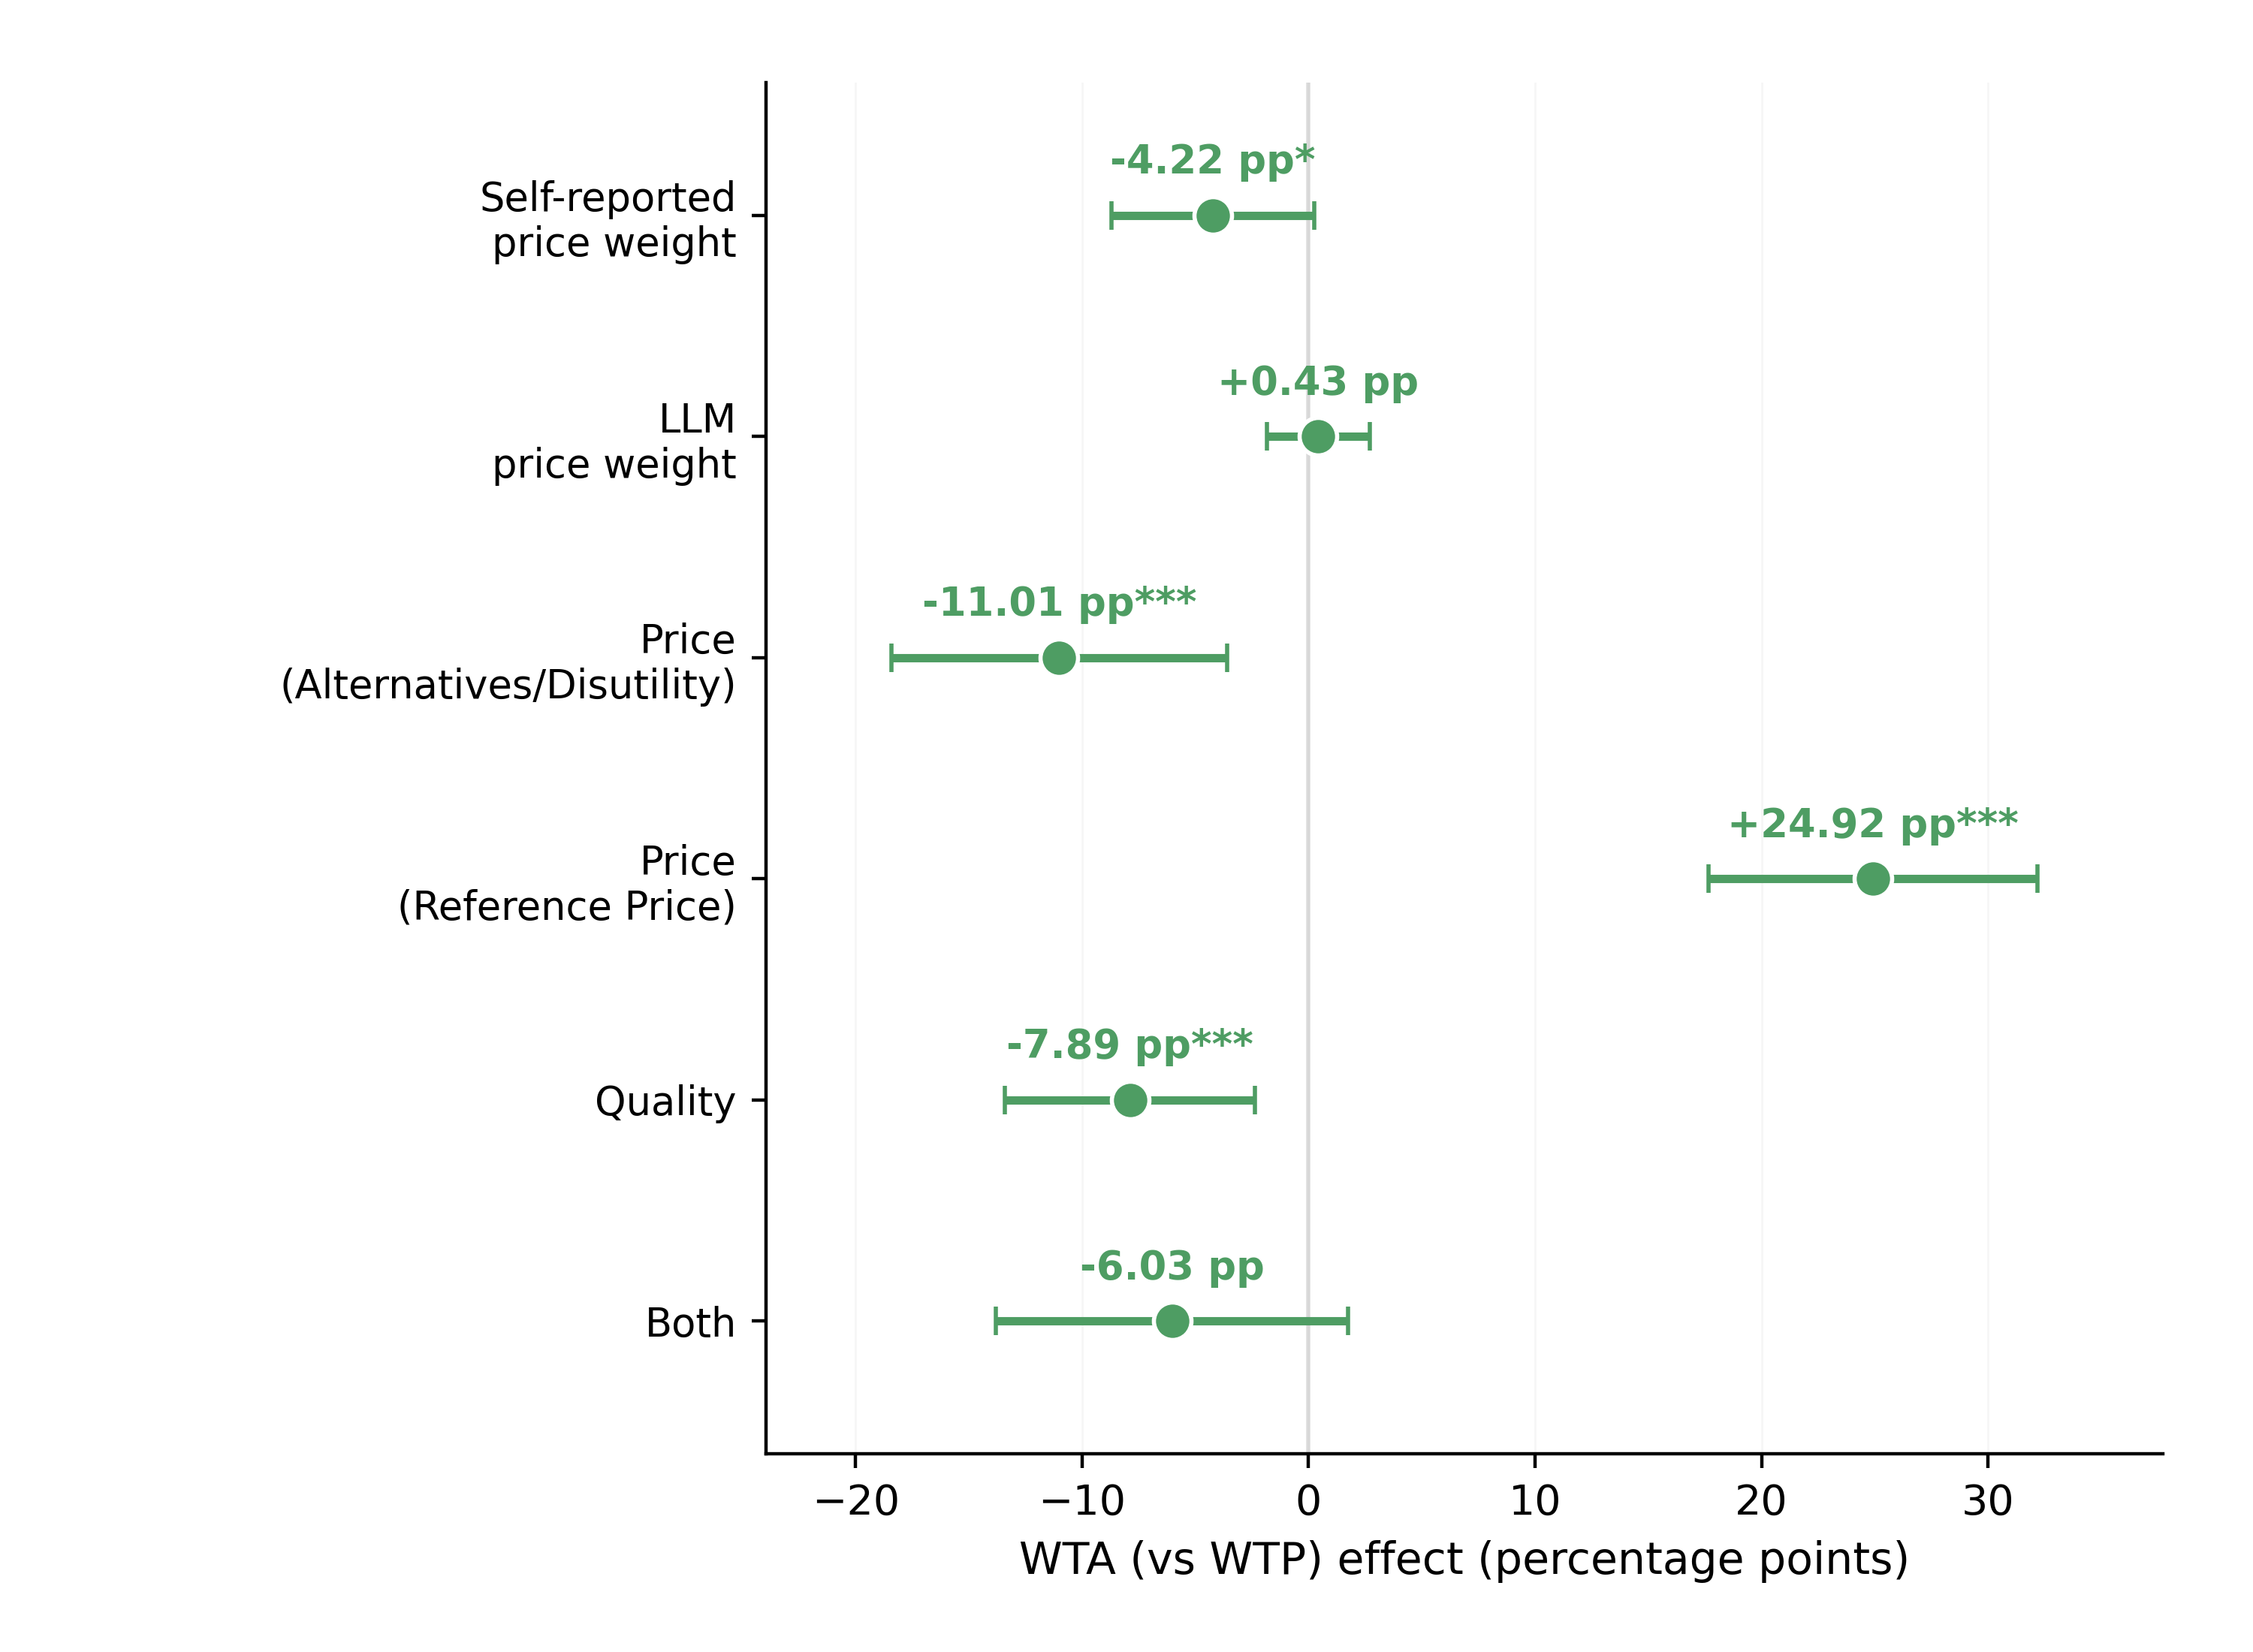
\includegraphics[width=0.82\linewidth]{figures/fig_wta_strong_llm_attention.png}
  \end{center}
\end{frame}


% ============================================================
\section{Heterogeneity}
% ============================================================

\begin{frame}{Heterogeneity: approach}
  \begin{itemize}
    \item Examine how two outcomes of interest vary with income and thrift: i) price elasticity, measured by premium take-up/valuation; and \\ii) WTA-WTP gap.
    \item Orthogonalize thrift within income brackets, and income within thrift brackets.
  \end{itemize}
\end{frame}

\begin{frame}{WTA-WTP gap: income}

WTA–WTP gap concentrates among lower-income respondents, driven by lower WTP.

  \begin{center}
    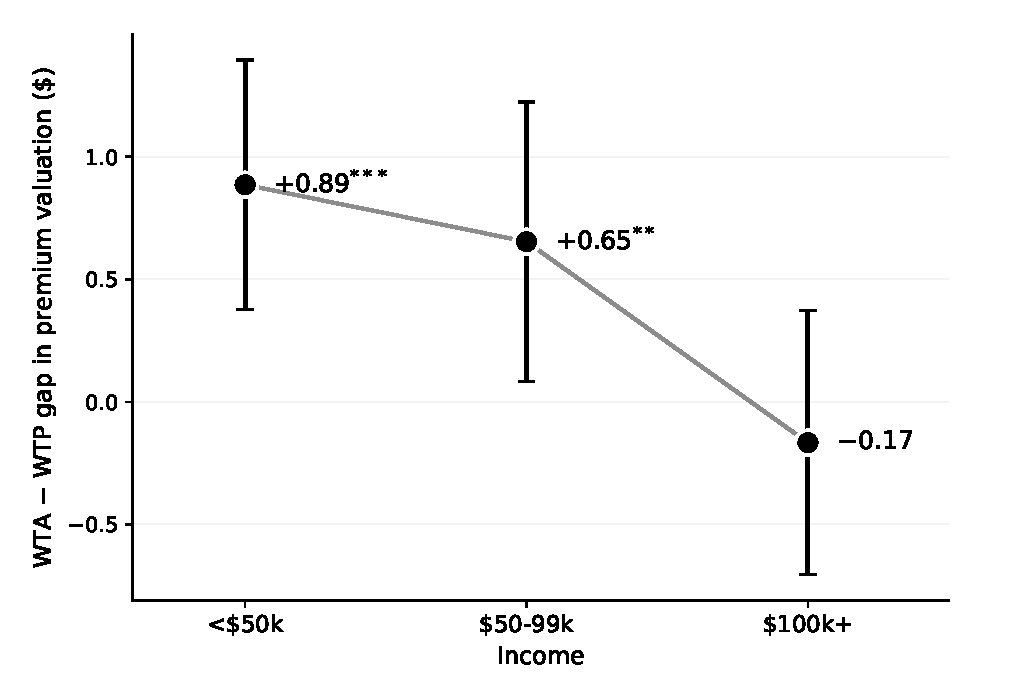
\includegraphics[width=0.55\textwidth]{figures/fig_result_gap_income.pdf}\hfill
    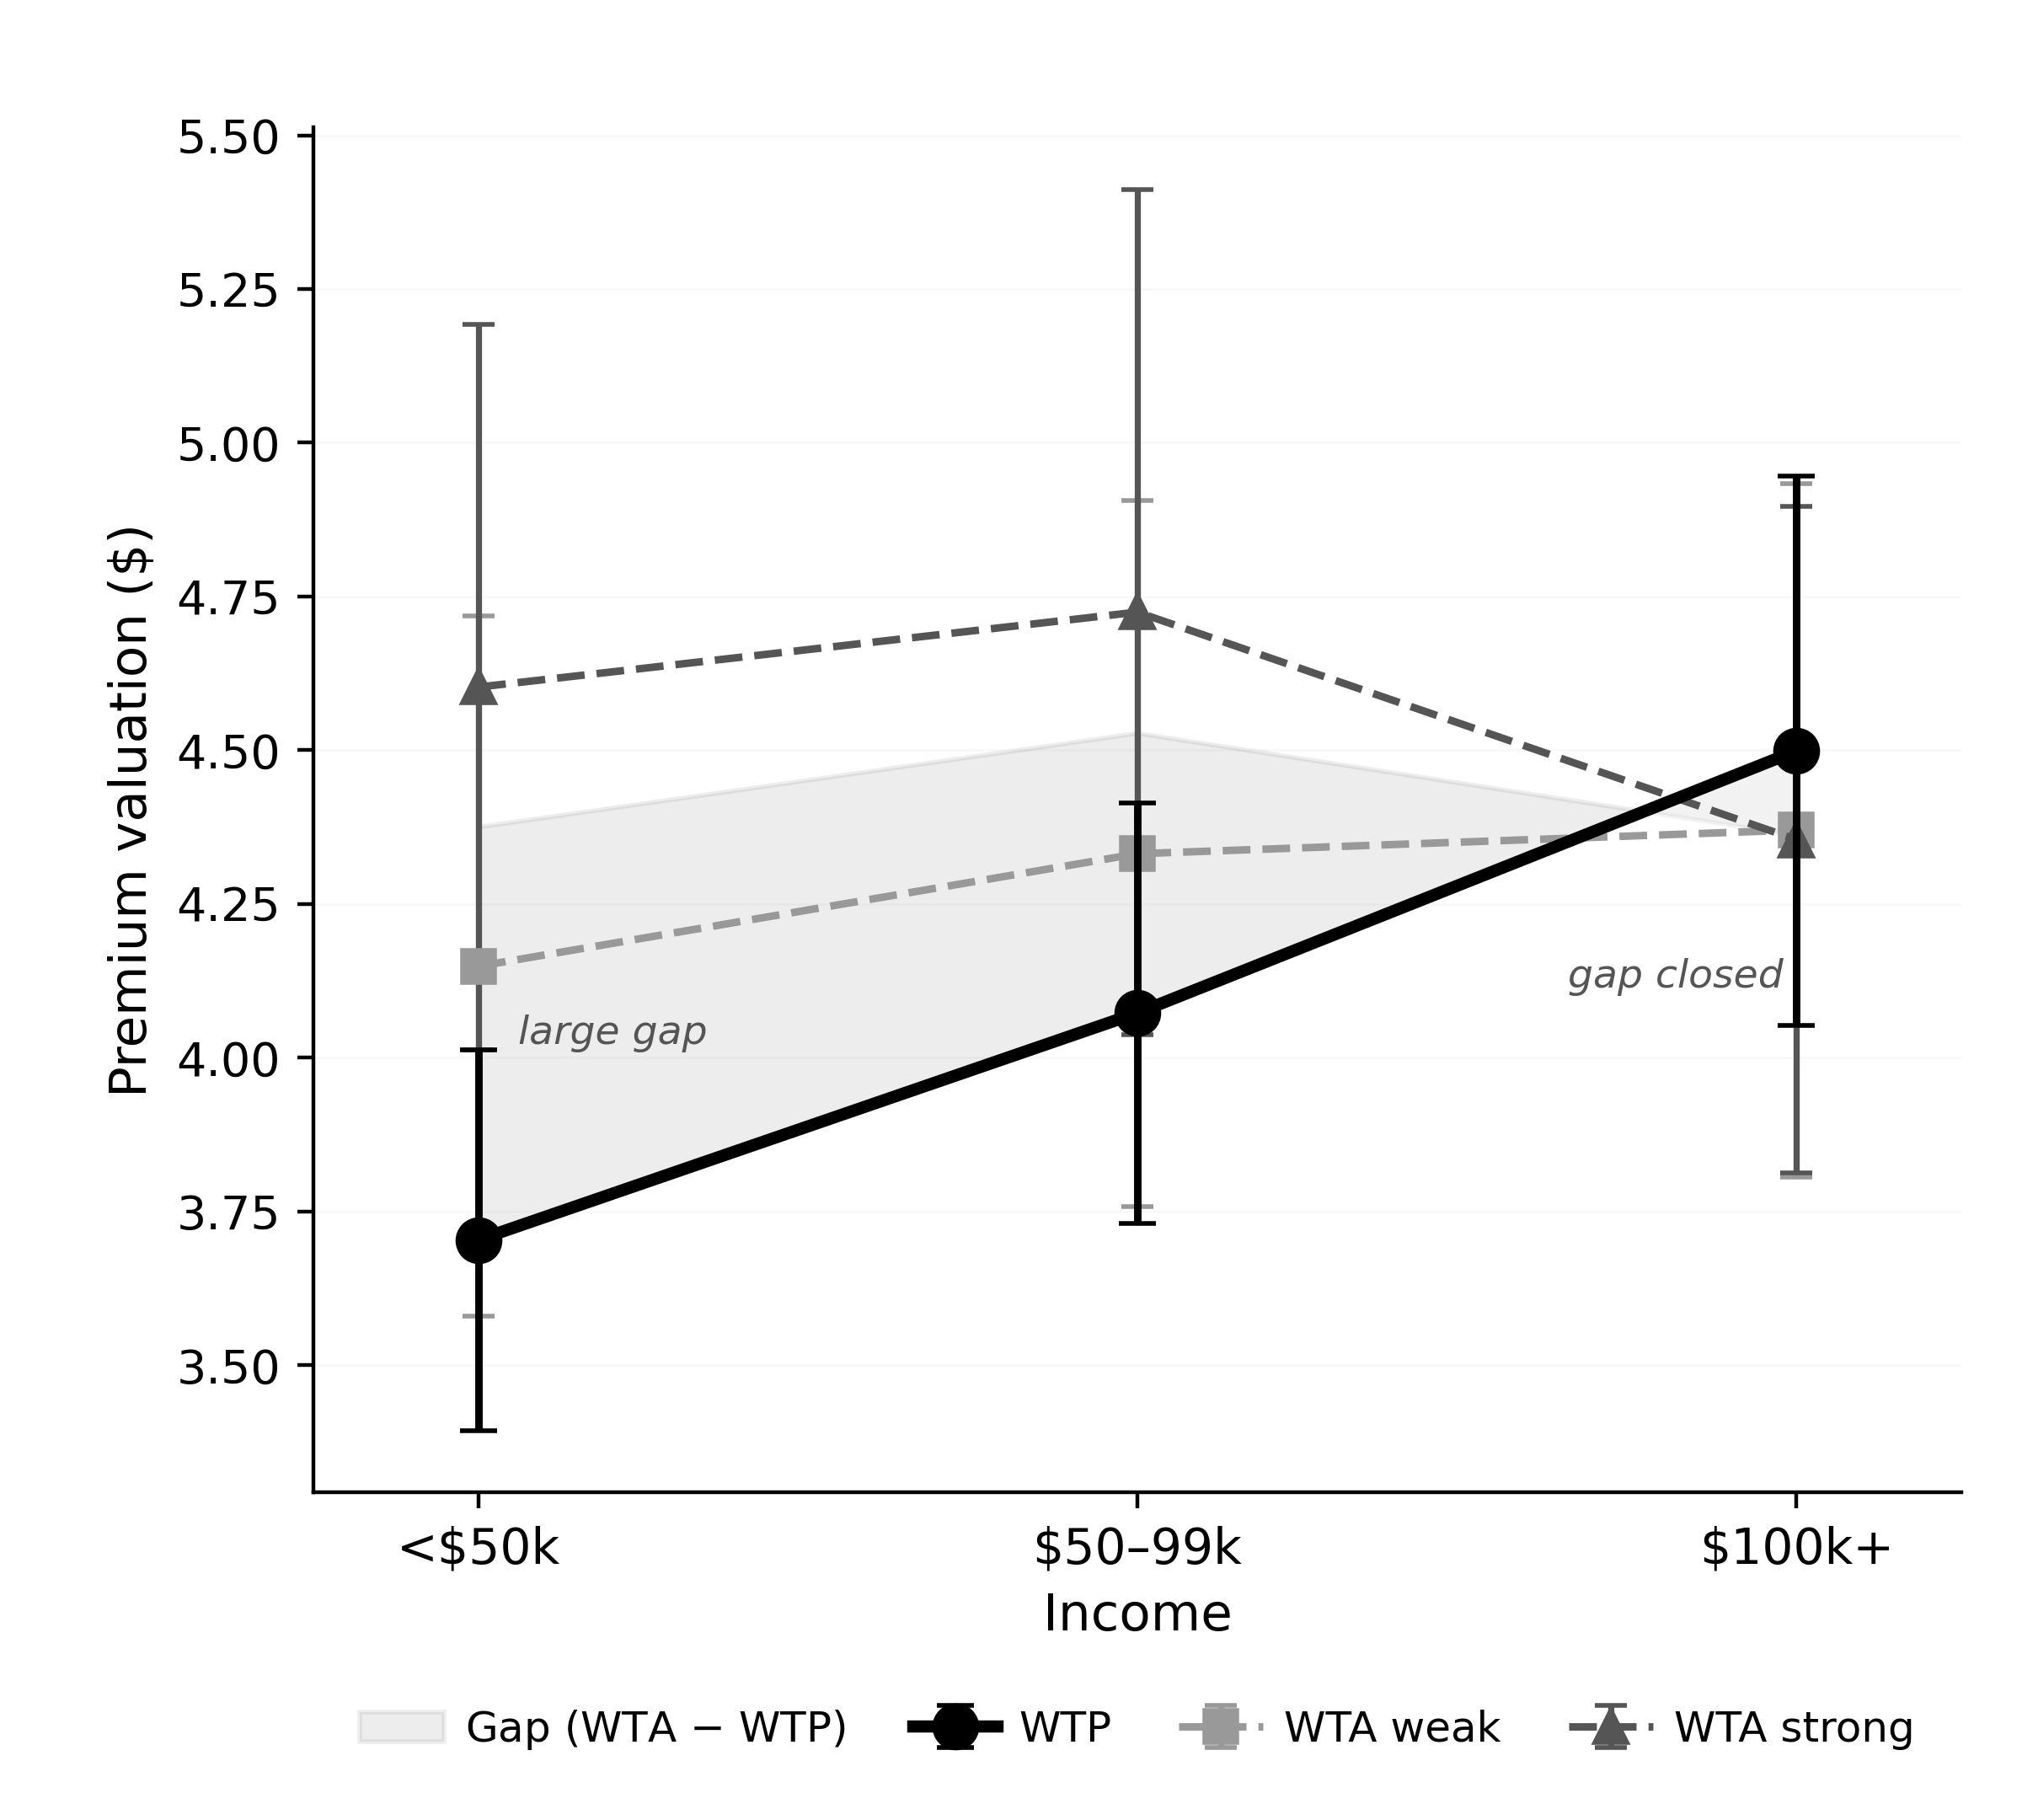
\includegraphics[width=0.45\textwidth]{figures/fig_gap_decomp.png}
  \end{center}

\end{frame}

\begin{frame}{WTA-WTP gap: thrift}

WTA–WTP gap concentrates among mid-thrift respondents.

  \begin{center}
    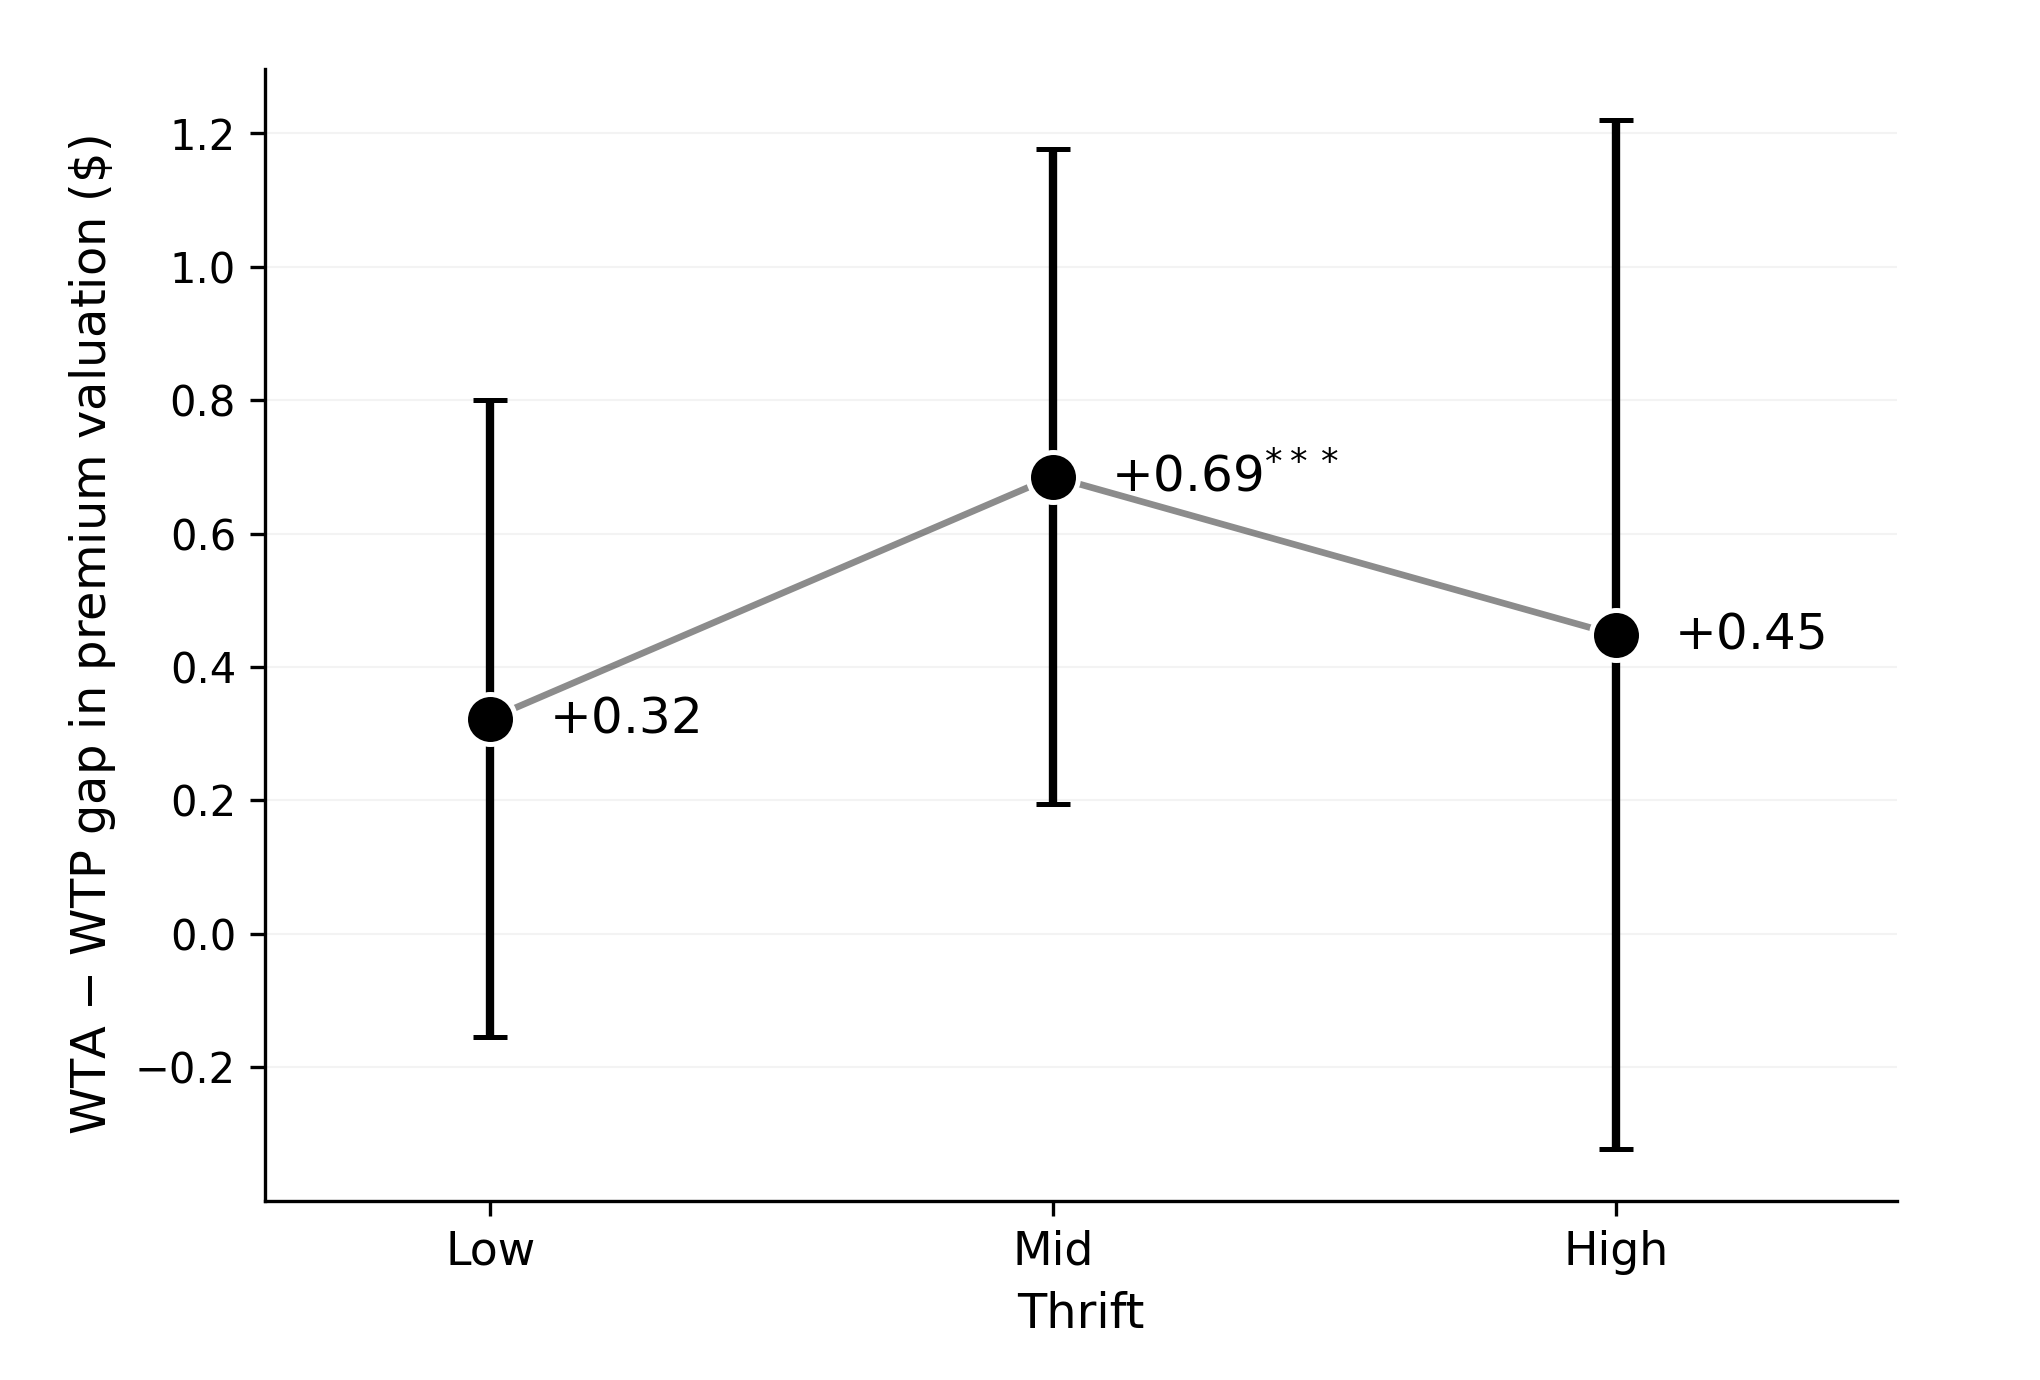
\includegraphics[width=0.55\textwidth]{figures/fig_result_gap_thrift.png}\hfill
    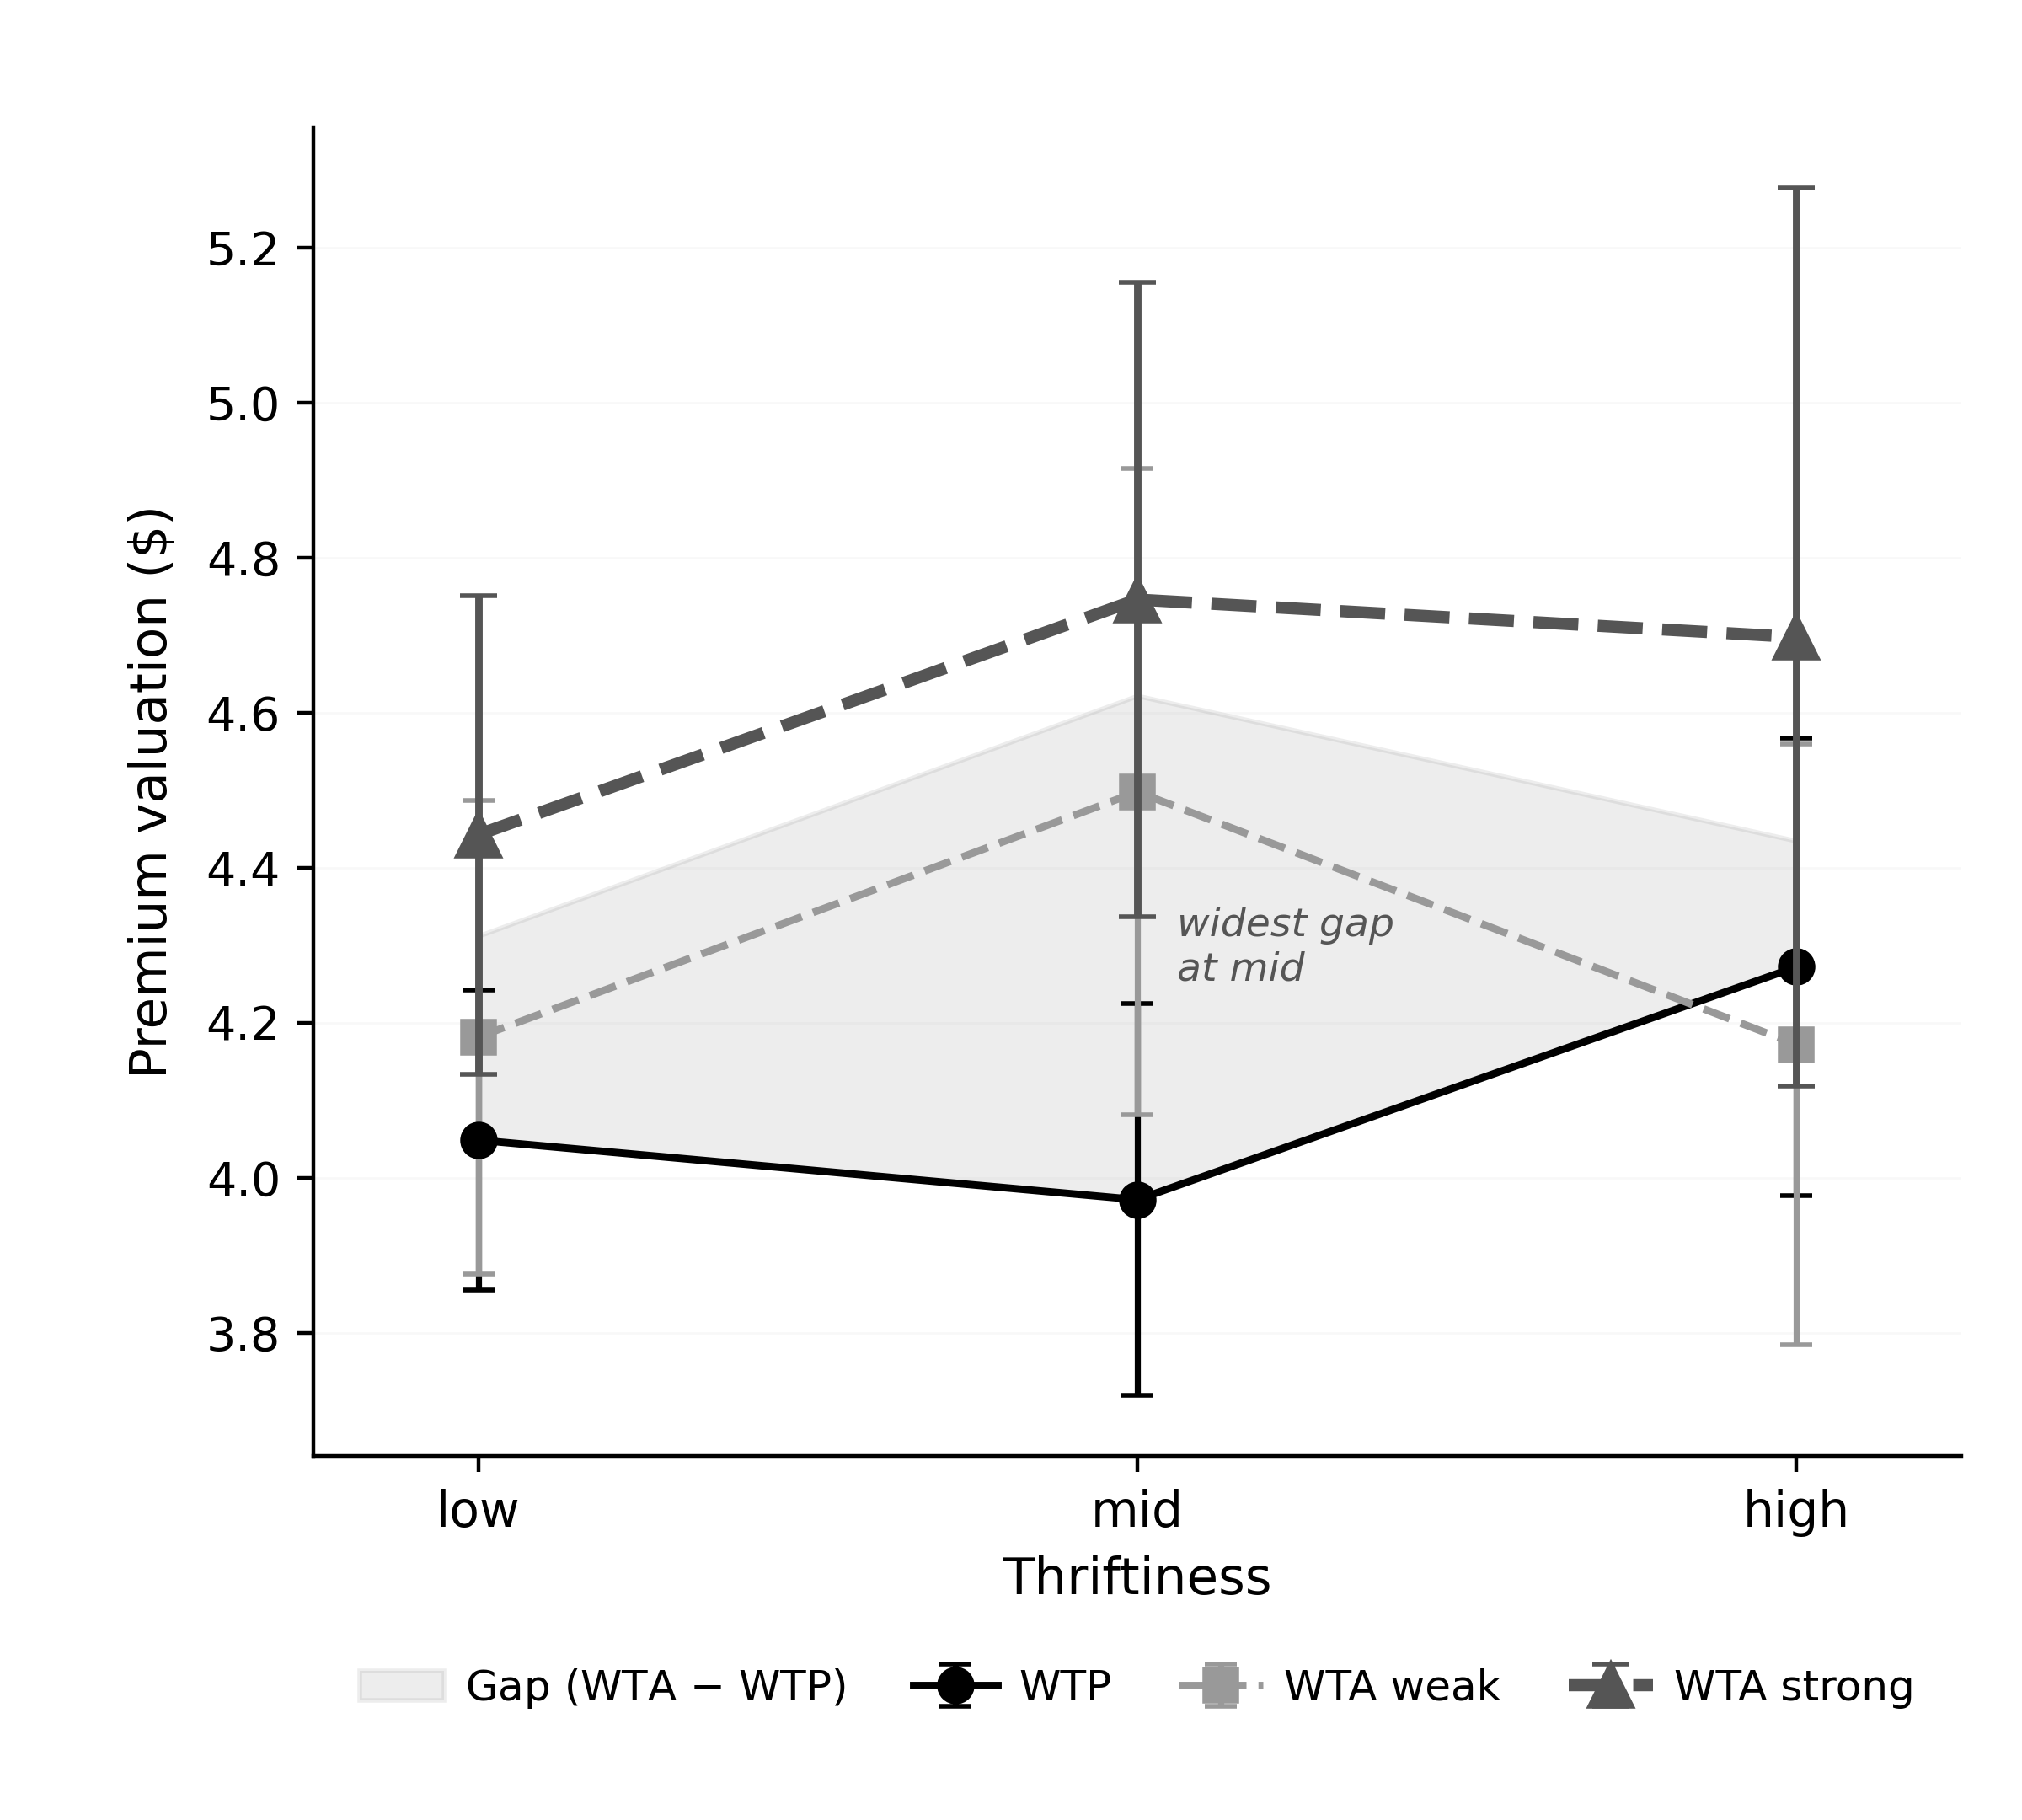
\includegraphics[width=0.45\textwidth]{figures/fig_gap_decomp_thrift.png}
  \end{center}

\end{frame}

 
% ---- Frame 2: thrift is a separate axis (Loewenstein) ----
\begin{frame}{Price elasticity: thrift (WTP within)}
People who think more carefully about money differentiate the premium more, but weight price no differently.
  \begin{center}
    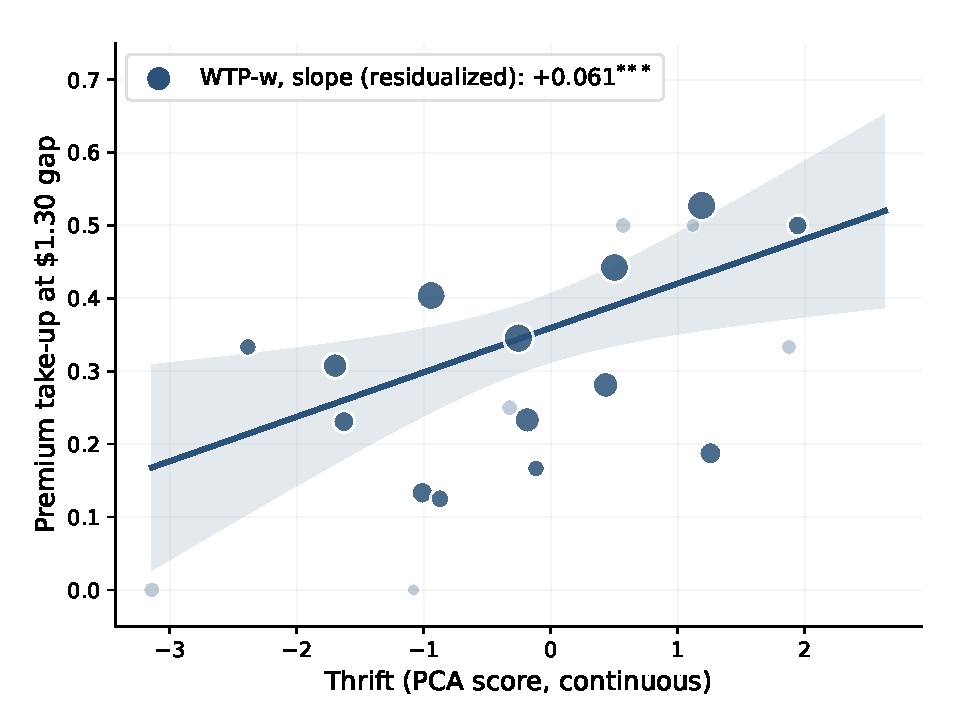
\includegraphics[width=0.49\textwidth]{figures/fig_het_wtp_thrift_continuous.pdf}\hfill
    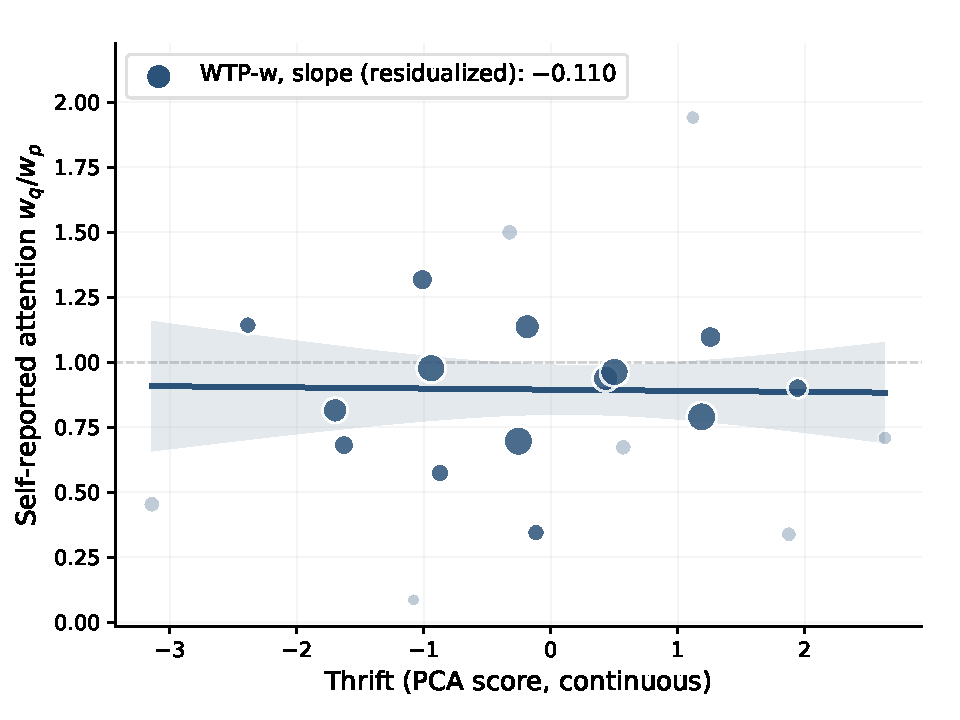
\includegraphics[width=0.49\textwidth]{figures/fig_het_wtp_thrift_attention.pdf}
  \end{center}
\end{frame}
 
% ---- Frame 3: orthogonalized income x thrift ----
\begin{frame}{\large Price elasticity: orthogonalized income $\times$ thrift (WTP within)}

Put income and thrift in same regression, and see which one predicts each outcome.

  \vspace{0.4em}
  \begin{center}
  \small
  \begin{tabular}{@{}lcc@{}}
    \toprule
     & Premium take-up & Premium valuation (\$) \\
    \cmidrule(lr){2-2}\cmidrule(lr){3-3}
    Income (bracket)      & $+0.050$        & $+0.415^{***}$ \\
                          & $(0.032)$       & $(0.121)$ \\
    \addlinespace[2pt]
    Thrift (PCA)          & $+0.063^{***}$  & $+0.043$ \\
                          & $(0.022)$       & $(0.075)$ \\
    \midrule
    Demographic controls  & Yes             & Yes \\
    Observations          & 397             & 397 \\
    \bottomrule
  \end{tabular}
  \end{center}
  \vspace{0.2em}
  {\footnotesize $\mathrm{corr}(\text{income},\text{thrift})=0.04$, uncorrelated.}


\end{frame}



\begin{frame}{\large Price elasticity: orthogonalized income $\times$ thrift (WTP within)}

Split thrift within each income half, and income within each thrift half.

\vspace{0.8em}
 
\begin{center}
\small
 
Premium take-up
\smallskip
 
\begin{tabular}{@{}lcc@{}}
\toprule
             & Thrift low & Thrift high \\
\midrule
Income low   & $0.28$ & $0.42$ \\
Income high  & $0.37$ & $0.41$ \\
\bottomrule
\end{tabular}
 
\bigskip
Premium valuation (\$)
\smallskip
 
\begin{tabular}{@{}lcc@{}}
\toprule
             & Thrift low & Thrift high \\
\midrule
Income low   & $3.87$ & $3.93$ \\
Income high  & $4.53$ & $4.40$ \\
\bottomrule
\end{tabular}

\end{center}

Income drives absolute valuation, thrift drives relative price sensitivity.

\end{frame}
 
% ---- Frame 4: consumption frame subgroups ----
\begin{frame}{Price elasticity (Binary, Consumption to Buying)}

Consumption frame acts mostly on high-income and middle-thrift respondents. (Suggestive: within-subgroup effects)

  \begin{center}
    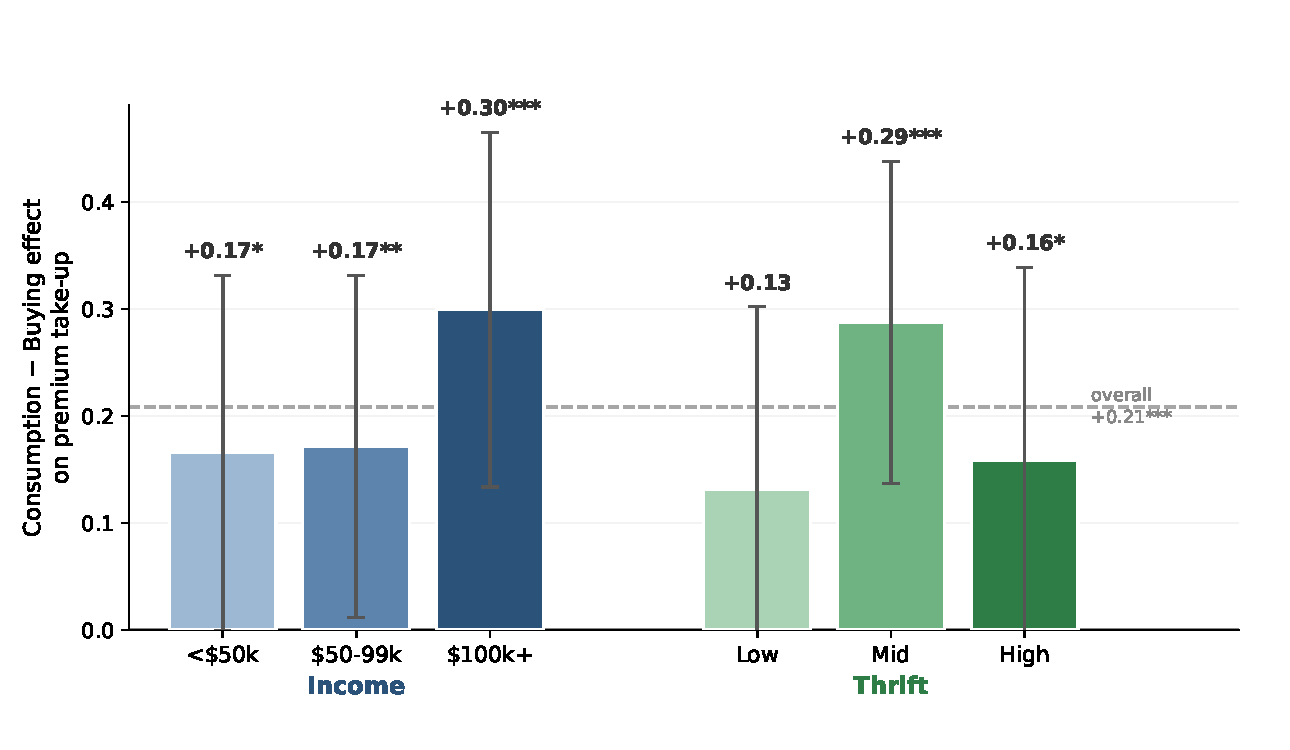
\includegraphics[width=0.86\textwidth]{figures/fig_consumption_binary.pdf}
  \end{center}


\end{frame}



% ============================================================

% ============================================================



% ============================================================
\appendix


\begin{frame}{Appendix: Cookie brands}
  \hypertarget{app:cookies_products}{}
  \backbutton{main:two_goods}
  \vspace{0.2cm}
  \begin{columns}
    \column{0.5\textwidth}
    \centering
    \textbf{Regular}\\[4pt]
    
\includegraphics[width=0.95\textwidth]{figures/cookies_regular.png}

    \column{0.5\textwidth}
    \centering
    \textbf{Premium}\\[4pt]
    
\includegraphics[width=0.95\textwidth]{figures/cookies_premium.png}
  \end{columns}
\end{frame}

\begin{frame}{Appendix: Toothpaste brands}
  \hypertarget{app:toothpaste_products}{}
  \backbutton{main:two_goods}
  \vspace{0.25cm}
  \begin{columns}
    \column{0.5\textwidth}
    \centering
    \textbf{Regular}\\[6pt]
    
\includegraphics[width=\textwidth]{figures/toothpaste_regular.png}

    \column{0.5\textwidth}
    \centering
    \textbf{Premium}\\[6pt]
    
\includegraphics[width=\textwidth]{figures/toothpaste_premium.png}
  \end{columns}
\end{frame}

\begin{frame}{Appendix: Control manipulation}
  \hypertarget{app:manipulation_control}{}
  \backbutton{main:binary_arms}
  \vspace{0.2cm}
  \begin{center}
    
\includegraphics[width=0.88\textwidth]{figures/manipulation_control.png}
  \end{center}
\end{frame}

\begin{frame}{Appendix: Buying manipulation}
  \hypertarget{app:manipulation_buying}{}
  \backbutton{main:binary_arms}
  \vspace{0.2cm}
  \begin{center}
    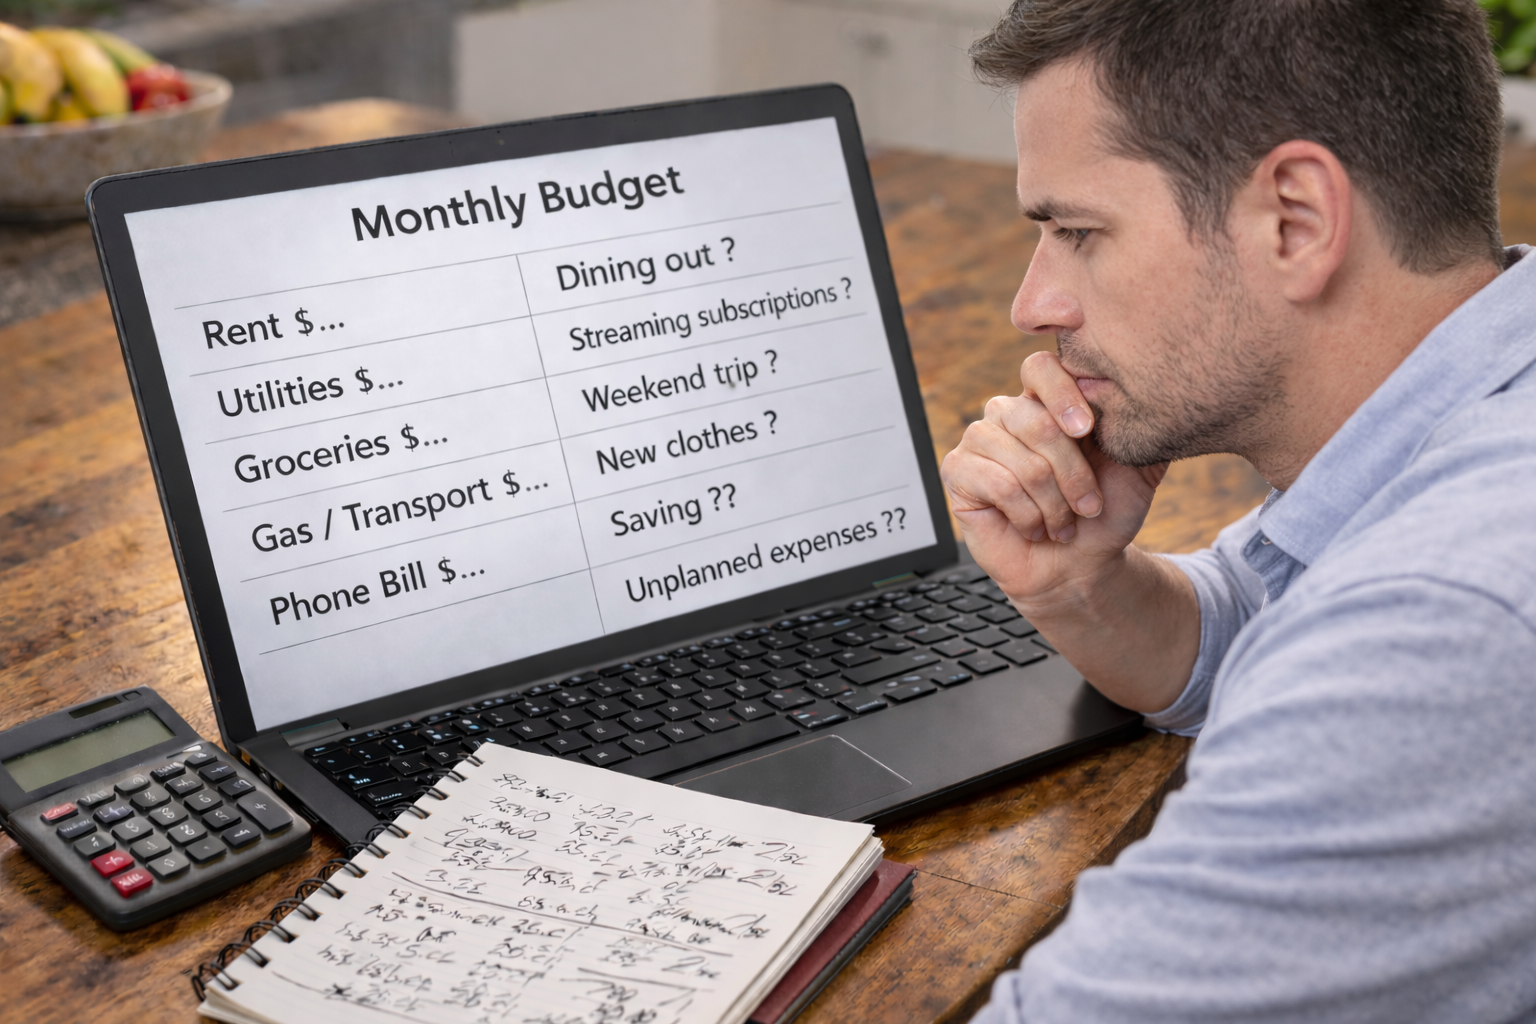
\includegraphics[width=0.88\textwidth]{figures/manipulation_buying.png}
  \end{center}
\end{frame}

\begin{frame}{Appendix: Consumption manipulation, cookies}
  \hypertarget{app:manipulation_consumption_cookies}{}
  \backbutton{main:binary_arms}
  \vspace{0.2cm}
  \begin{center}
    
\includegraphics[height=0.72\textheight]{figures/manipulation_consumption_cookies.png}
  \end{center}
\end{frame}

\begin{frame}{Appendix: Consumption manipulation, toothpaste}
  \hypertarget{app:manipulation_consumption_toothpaste}{}
  \backbutton{main:binary_arms}
  \vspace{0.2cm}
  \begin{center}
    
\includegraphics[height=0.72\textheight]{figures/manipulation_consumption.png}
  \end{center}
\end{frame}

\begin{frame}{Appendix: Functionality by product}
  \hypertarget{app:functionality_compare}{}
  \backbutton{main:two_goods}
  \vspace{0.15cm}
  \begin{center}
    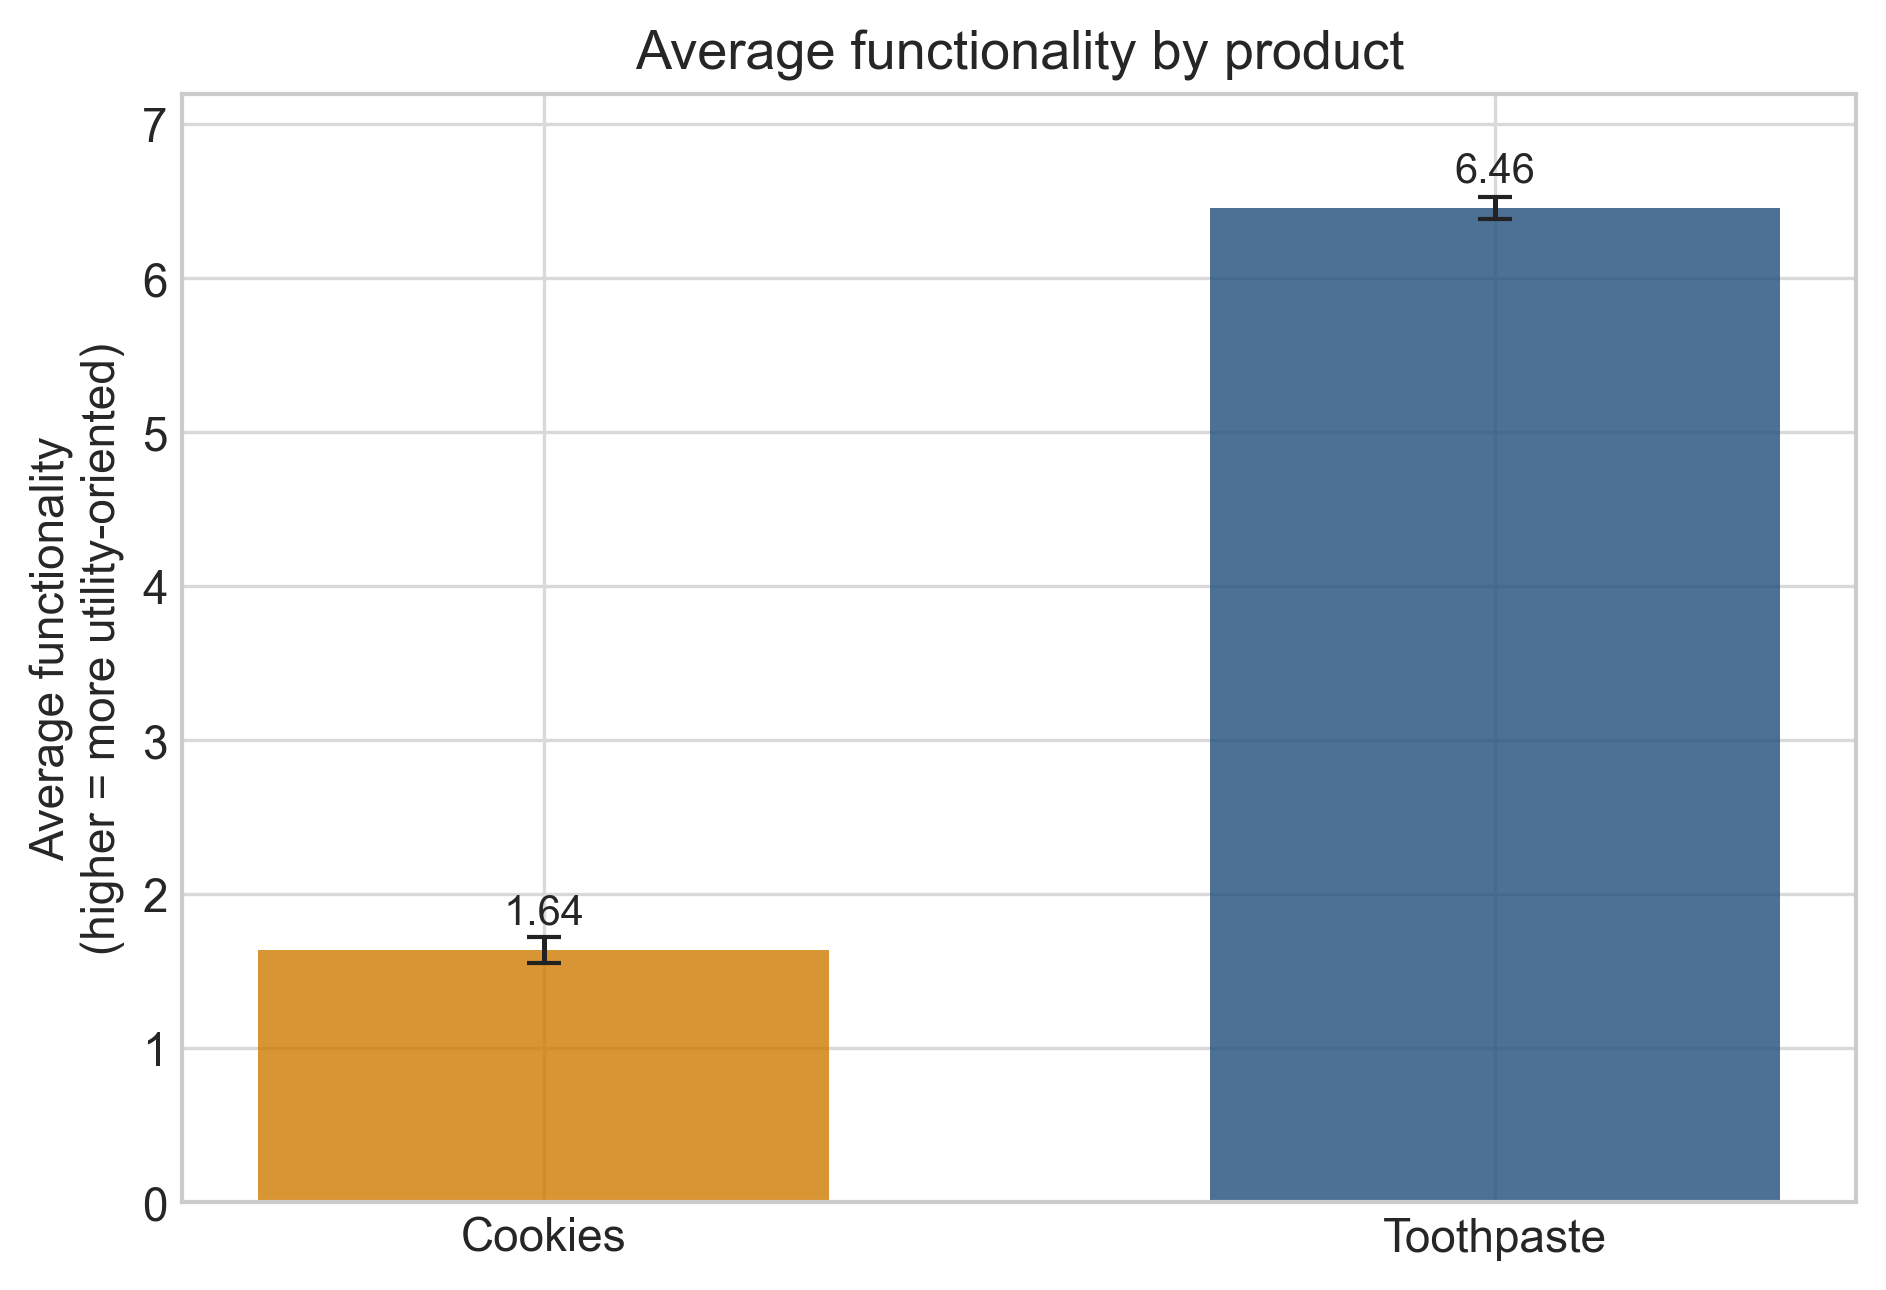
\includegraphics[width=0.72\textwidth]{figures/cookies_toothpaste_functionality_comparison.png}
  \end{center}
  \vspace{0.1cm}
  {\footnotesize
  Question used:

  ``In your everyday life, do you purchase PRODUCTNAME predominantly for pleasure or for its utility?''}
\end{frame}

\begin{frame}{Appendix: WTP within attention, multiple-choice version}
  \hypertarget{app:wtp_within_attention_multiple_choice}{}
  \backbutton{main:wtp_within_attention}
  \vspace{0.2cm}
  \begin{columns}
    \column{0.5\textwidth}
    \centering
    Cookies\\[2pt]
    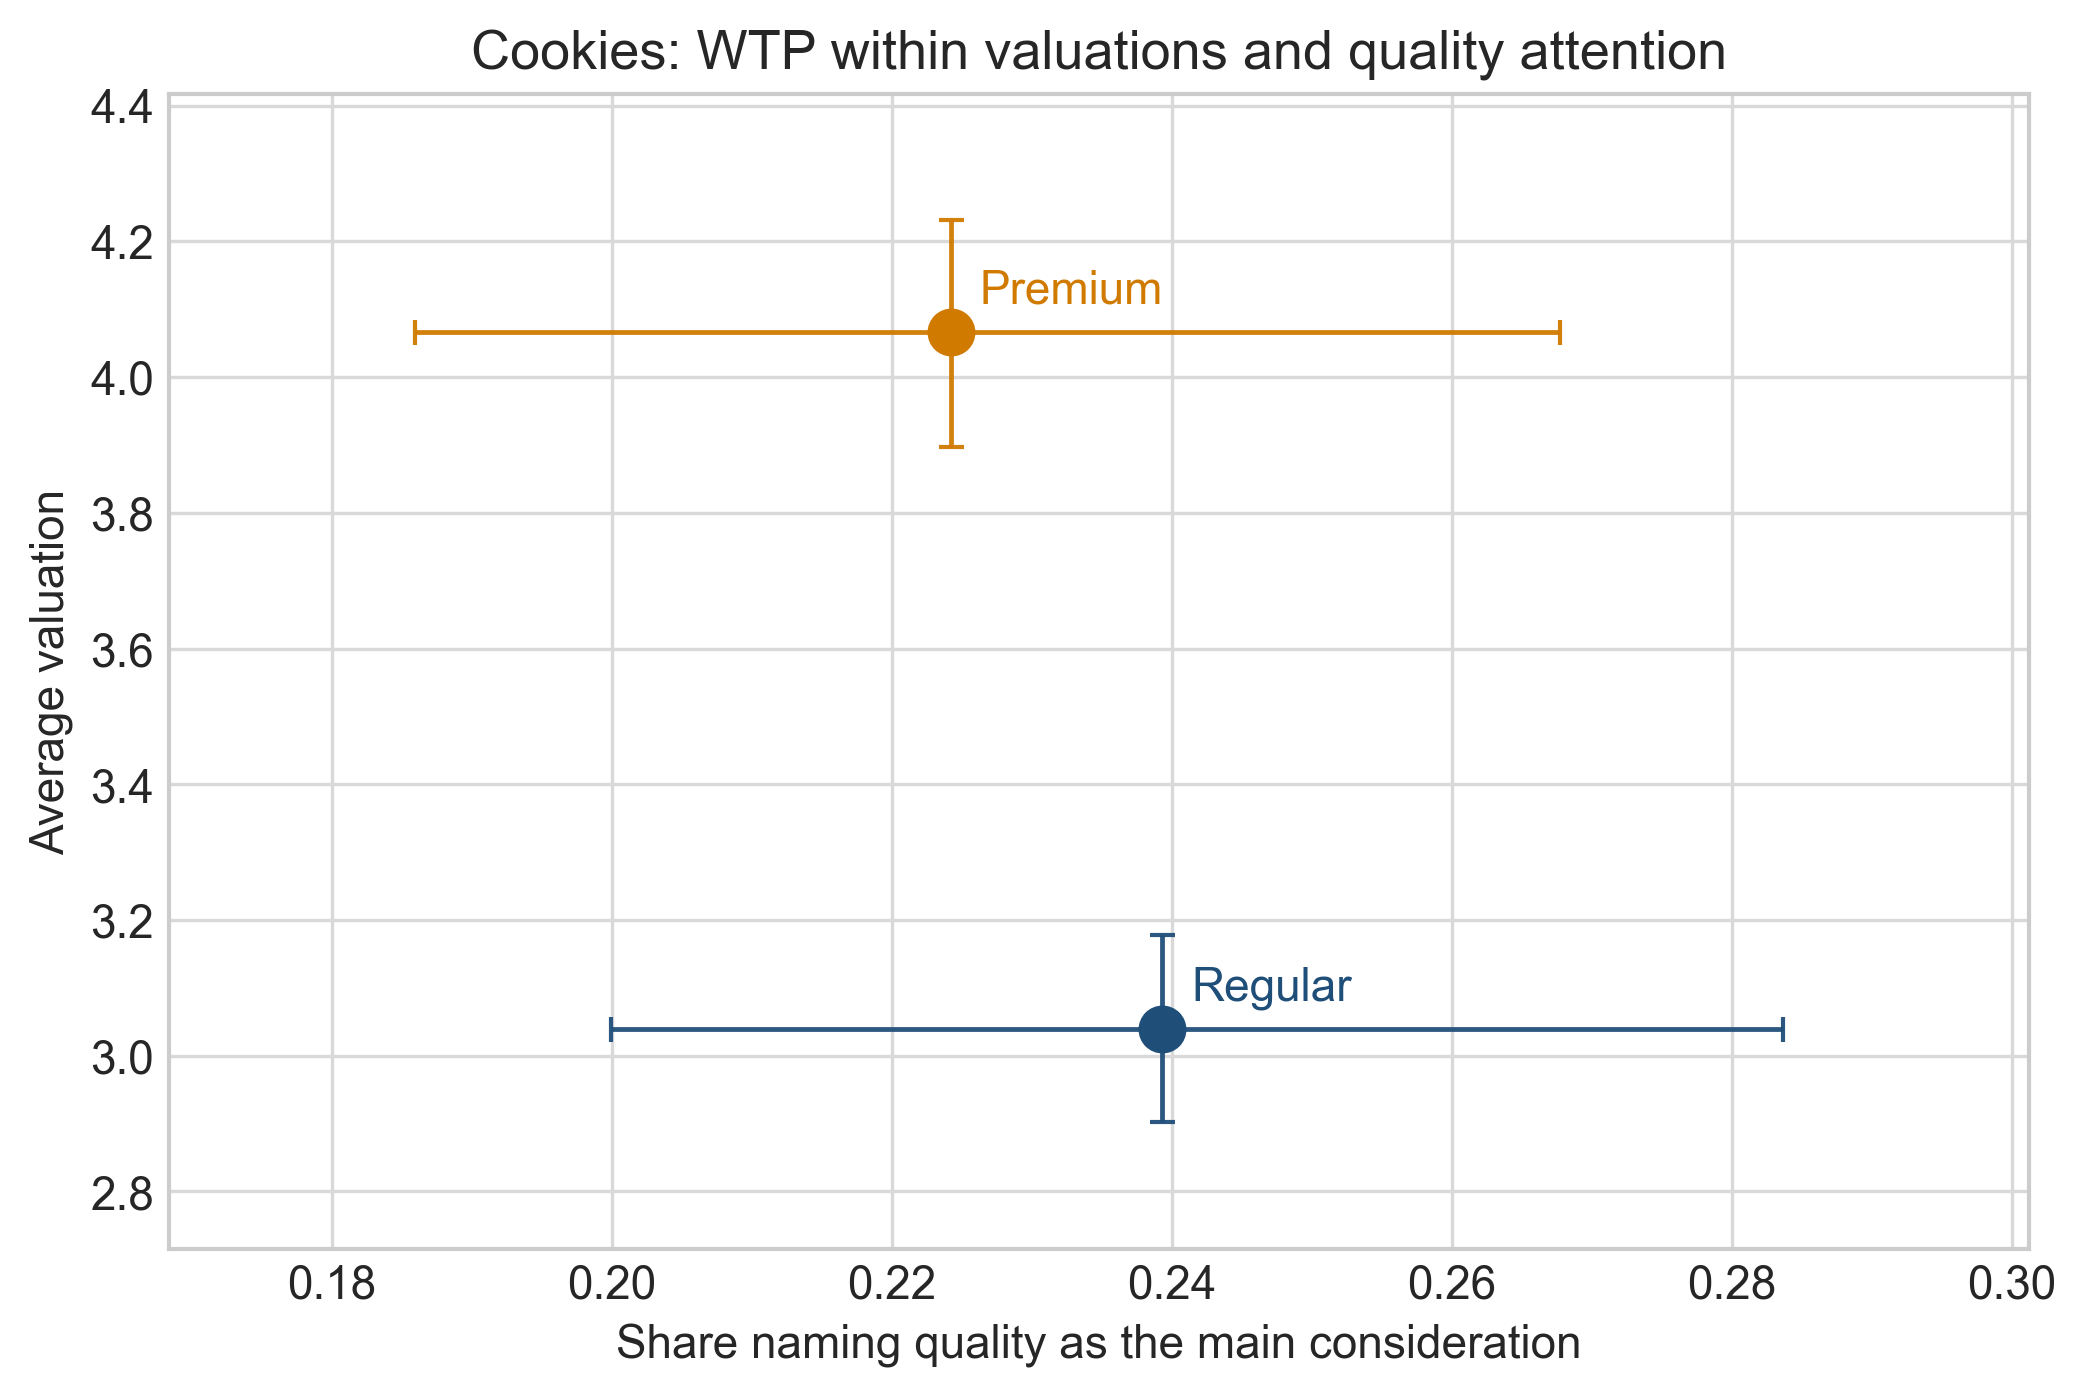
\includegraphics[width=\textwidth]{figures/wtp_within_cookies_quality_share_vs_price.png}

    \column{0.5\textwidth}
    \centering
    Toothpaste\\[2pt]
    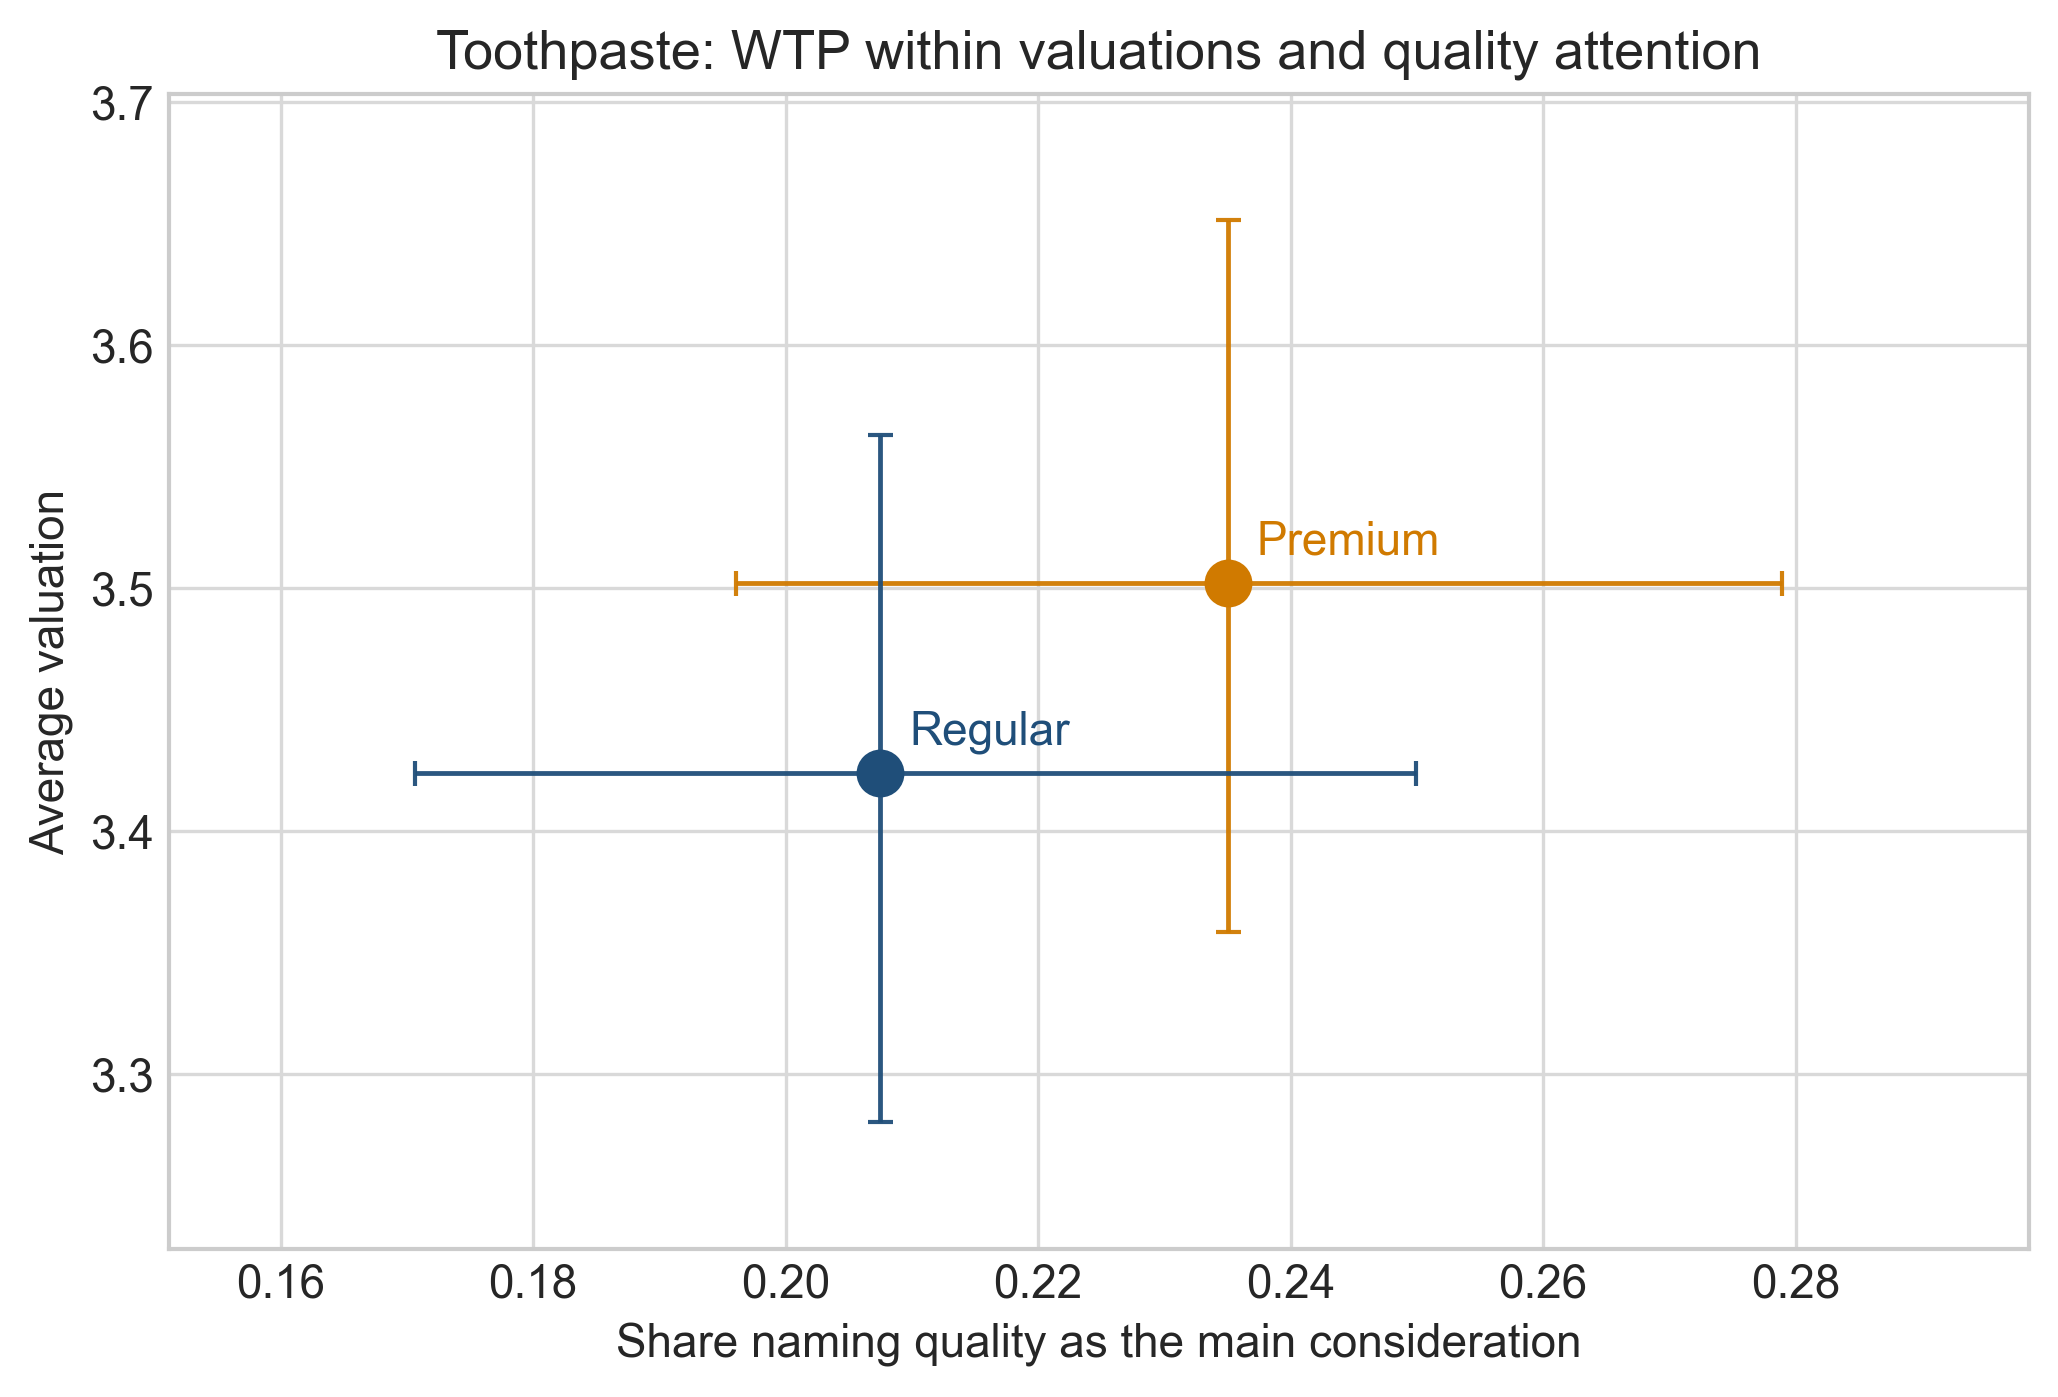
\includegraphics[width=\textwidth]{figures/wtp_within_toothpaste_quality_share_vs_price.png}
  \end{columns}
\end{frame}

\begin{frame}{Appendix: WTP within attention and implied premium take-up}
  \hypertarget{app:wtp_takeup_reg}{}
  \backbutton{main:wtp_gap_reg}

\centering
\tiny
\renewcommand{\arraystretch}{0.92}\setlength{\tabcolsep}{3pt}
\begin{tabular}{@{}l*{7}{c}@{}}
\toprule
 & \multicolumn{7}{c}{$\mathbf{1}\{\text{premium}-\text{regular} \geq \$1.30\}$} \\
\cmidrule(lr){2-8}
 & (1) & (2) & (3) & (4) & (5) & (6) & (7) \\
\midrule
$\omega^{SR}_p$              & $-0.005$\sym{***} &                    & $-0.004$\sym{***} &                    &                   & $-0.002$\sym{**}  & $-0.003$\sym{**}  \\
                             & (0.001)           &                    & (0.001)           &                    &                   & (0.001)           & (0.001)           \\[1pt]
\addlinespace[2pt]
\multicolumn{8}{@{}l}{Self-reported category \quad (base: Price)} \\
\addlinespace[1pt]
\quad Quality                &                   & $\phantom{-}0.227$\sym{***} & $\phantom{-}0.026$ &                    &                   &                   & $-0.095$          \\
                             &                   & (0.064)            & (0.082)            &                    &                   &                   & (0.079)           \\[1pt]
\quad Both                   &                   & $\phantom{-}0.145$\sym{***} & $\phantom{-}0.054$ &                    &                   &                   & $-0.007$          \\
                             &                   & (0.054)            & (0.058)            &                    &                   &                   & (0.057)           \\[1pt]
$\omega^{LLM}_p$             &                   &                    &                   & $-0.011$\sym{***} & $-0.005$\sym{*}   & $-0.003$          & $-0.004$          \\
                             &                   &                    &                   & (0.002)           & (0.003)           & (0.003)           & (0.003)           \\[1pt]
\addlinespace[2pt]
\multicolumn{8}{@{}l}{LLM labelled category \quad (base: Price Alternatives/Disutility)} \\
\addlinespace[1pt]
\quad Price (Reference Price)&                   &                    &                   &                    & $\phantom{-}0.187$\sym{**} & $\phantom{-}0.179$\sym{**} & $\phantom{-}0.170$\sym{**} \\
                             &                   &                    &                   &                    & (0.086)           & (0.086)           & (0.086)           \\[1pt]
\quad Quality                &                   &                    &                   &                    & $\phantom{-}0.196$\sym{*}  & $\phantom{-}0.190$ & $\phantom{-}0.190$ \\
                             &                   &                    &                   &                    & (0.118)           & (0.118)           & (0.118)           \\[1pt]
\quad Both                   &                   &                    &                   &                    & $\phantom{-}0.155$\sym{**} & $\phantom{-}0.149$\sym{**} & $\phantom{-}0.145$\sym{**} \\
                             &                   &                    &                   &                    & (0.067)           & (0.067)           & (0.067)           \\[1pt]
\addlinespace[2pt]
\multicolumn{8}{@{}l}{LLM labelled valence \quad (base: Price Too High)} \\
\addlinespace[1pt]
\quad Quality Too Low        &                   &                    &                   &                    & $-0.203$          & $-0.224$\sym{*}   & $-0.210$          \\
                             &                   &                    &                   &                    & (0.129)           & (0.129)           & (0.128)           \\[1pt]
\quad Price Too Low          &                   &                    &                   &                    & $-0.002$          & $-0.012$          & $-0.005$          \\
                             &                   &                    &                   &                    & (0.078)           & (0.077)           & (0.077)           \\[1pt]
\quad Quality Too High       &                   &                    &                   &                    & $\phantom{-}0.124$ & $\phantom{-}0.114$ & $\phantom{-}0.123$ \\
                             &                   &                    &                   &                    & (0.102)           & (0.101)           & (0.101)           \\[1pt]
\midrule
Controls (demog.\ \& thrift) & Yes & Yes & Yes & Yes & Yes & Yes & Yes \\
Adj.\ $R^2$                  & 0.076 & 0.041 & 0.073 & 0.125 & 0.141 & 0.149 & 0.148 \\
Observations                 & 387 & 387 & 387 & 387 & 387 & 387 & 387 \\
\bottomrule
\end{tabular}
\end{frame}

\begin{frame}{Appendix: WTA attention, multiple-choice version}
  \hypertarget{app:wta_attention_multiple_choice}{}
  \backbutton{main:wta_attention}
  \vspace{0.2cm}
  \begin{center}
    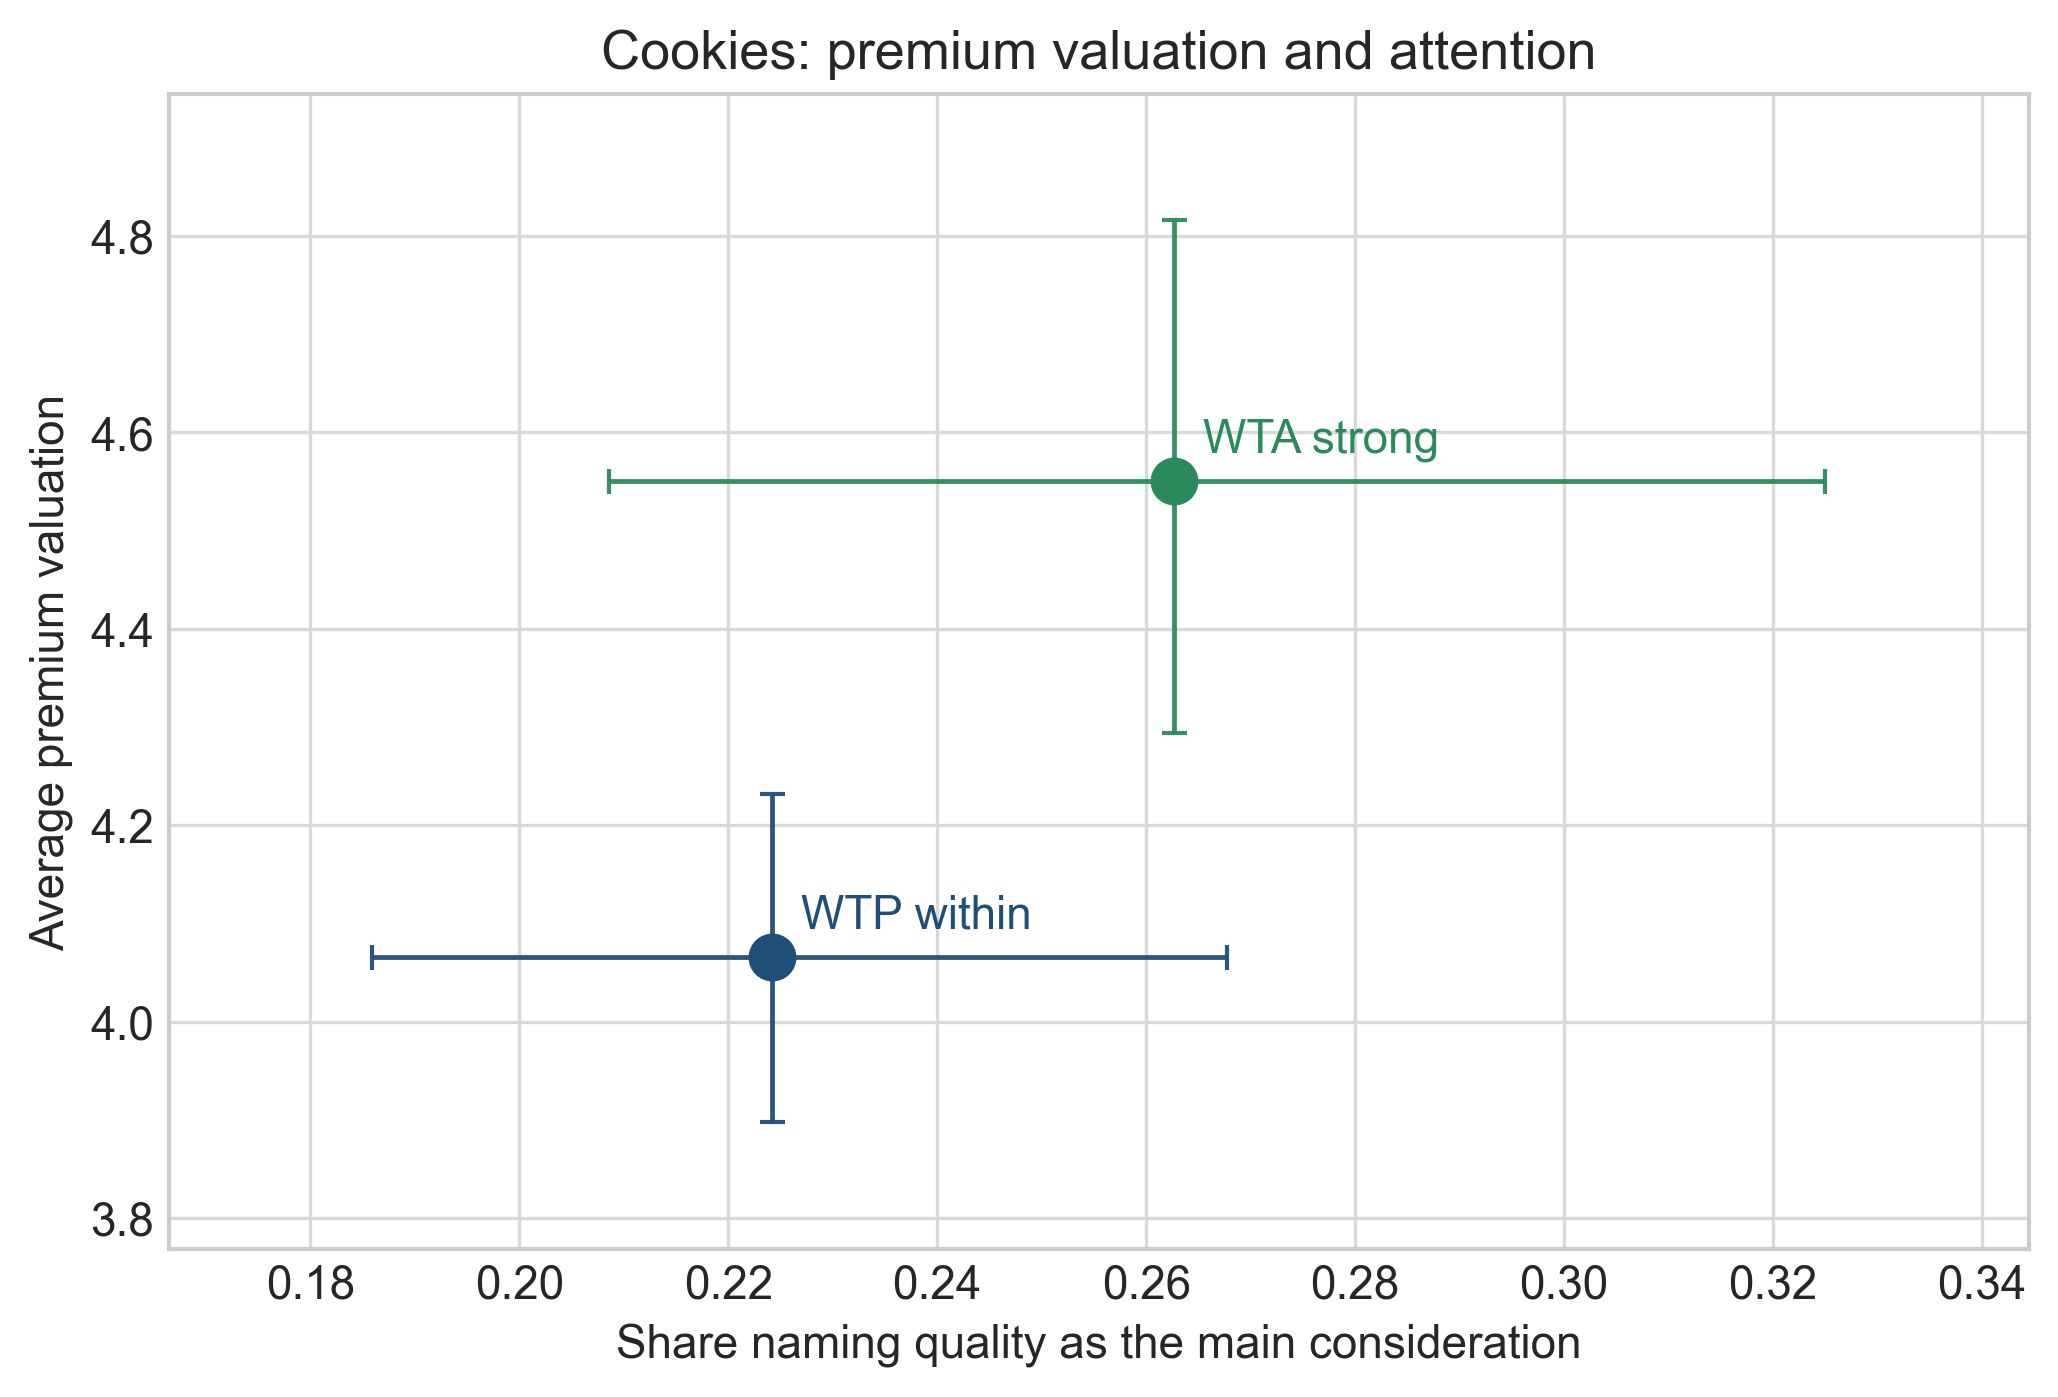
\includegraphics[width=0.75\textwidth]{figures/wta_strong_cookies_quality_share_vs_price.png}
  \end{center}
\end{frame}

\begin{frame}{Appendix: Observed vs.\ attention-predicted WTA\,$-$\,WTP gap}
  \hypertarget{app:wta_gap_predicted}{}
  \backbutton{main:wta_combined}
 
\raggedright
{
Predict premium valuation from attention alone, take the WTA--WTP difference in means.}
 
\vspace{2pt}
\noindent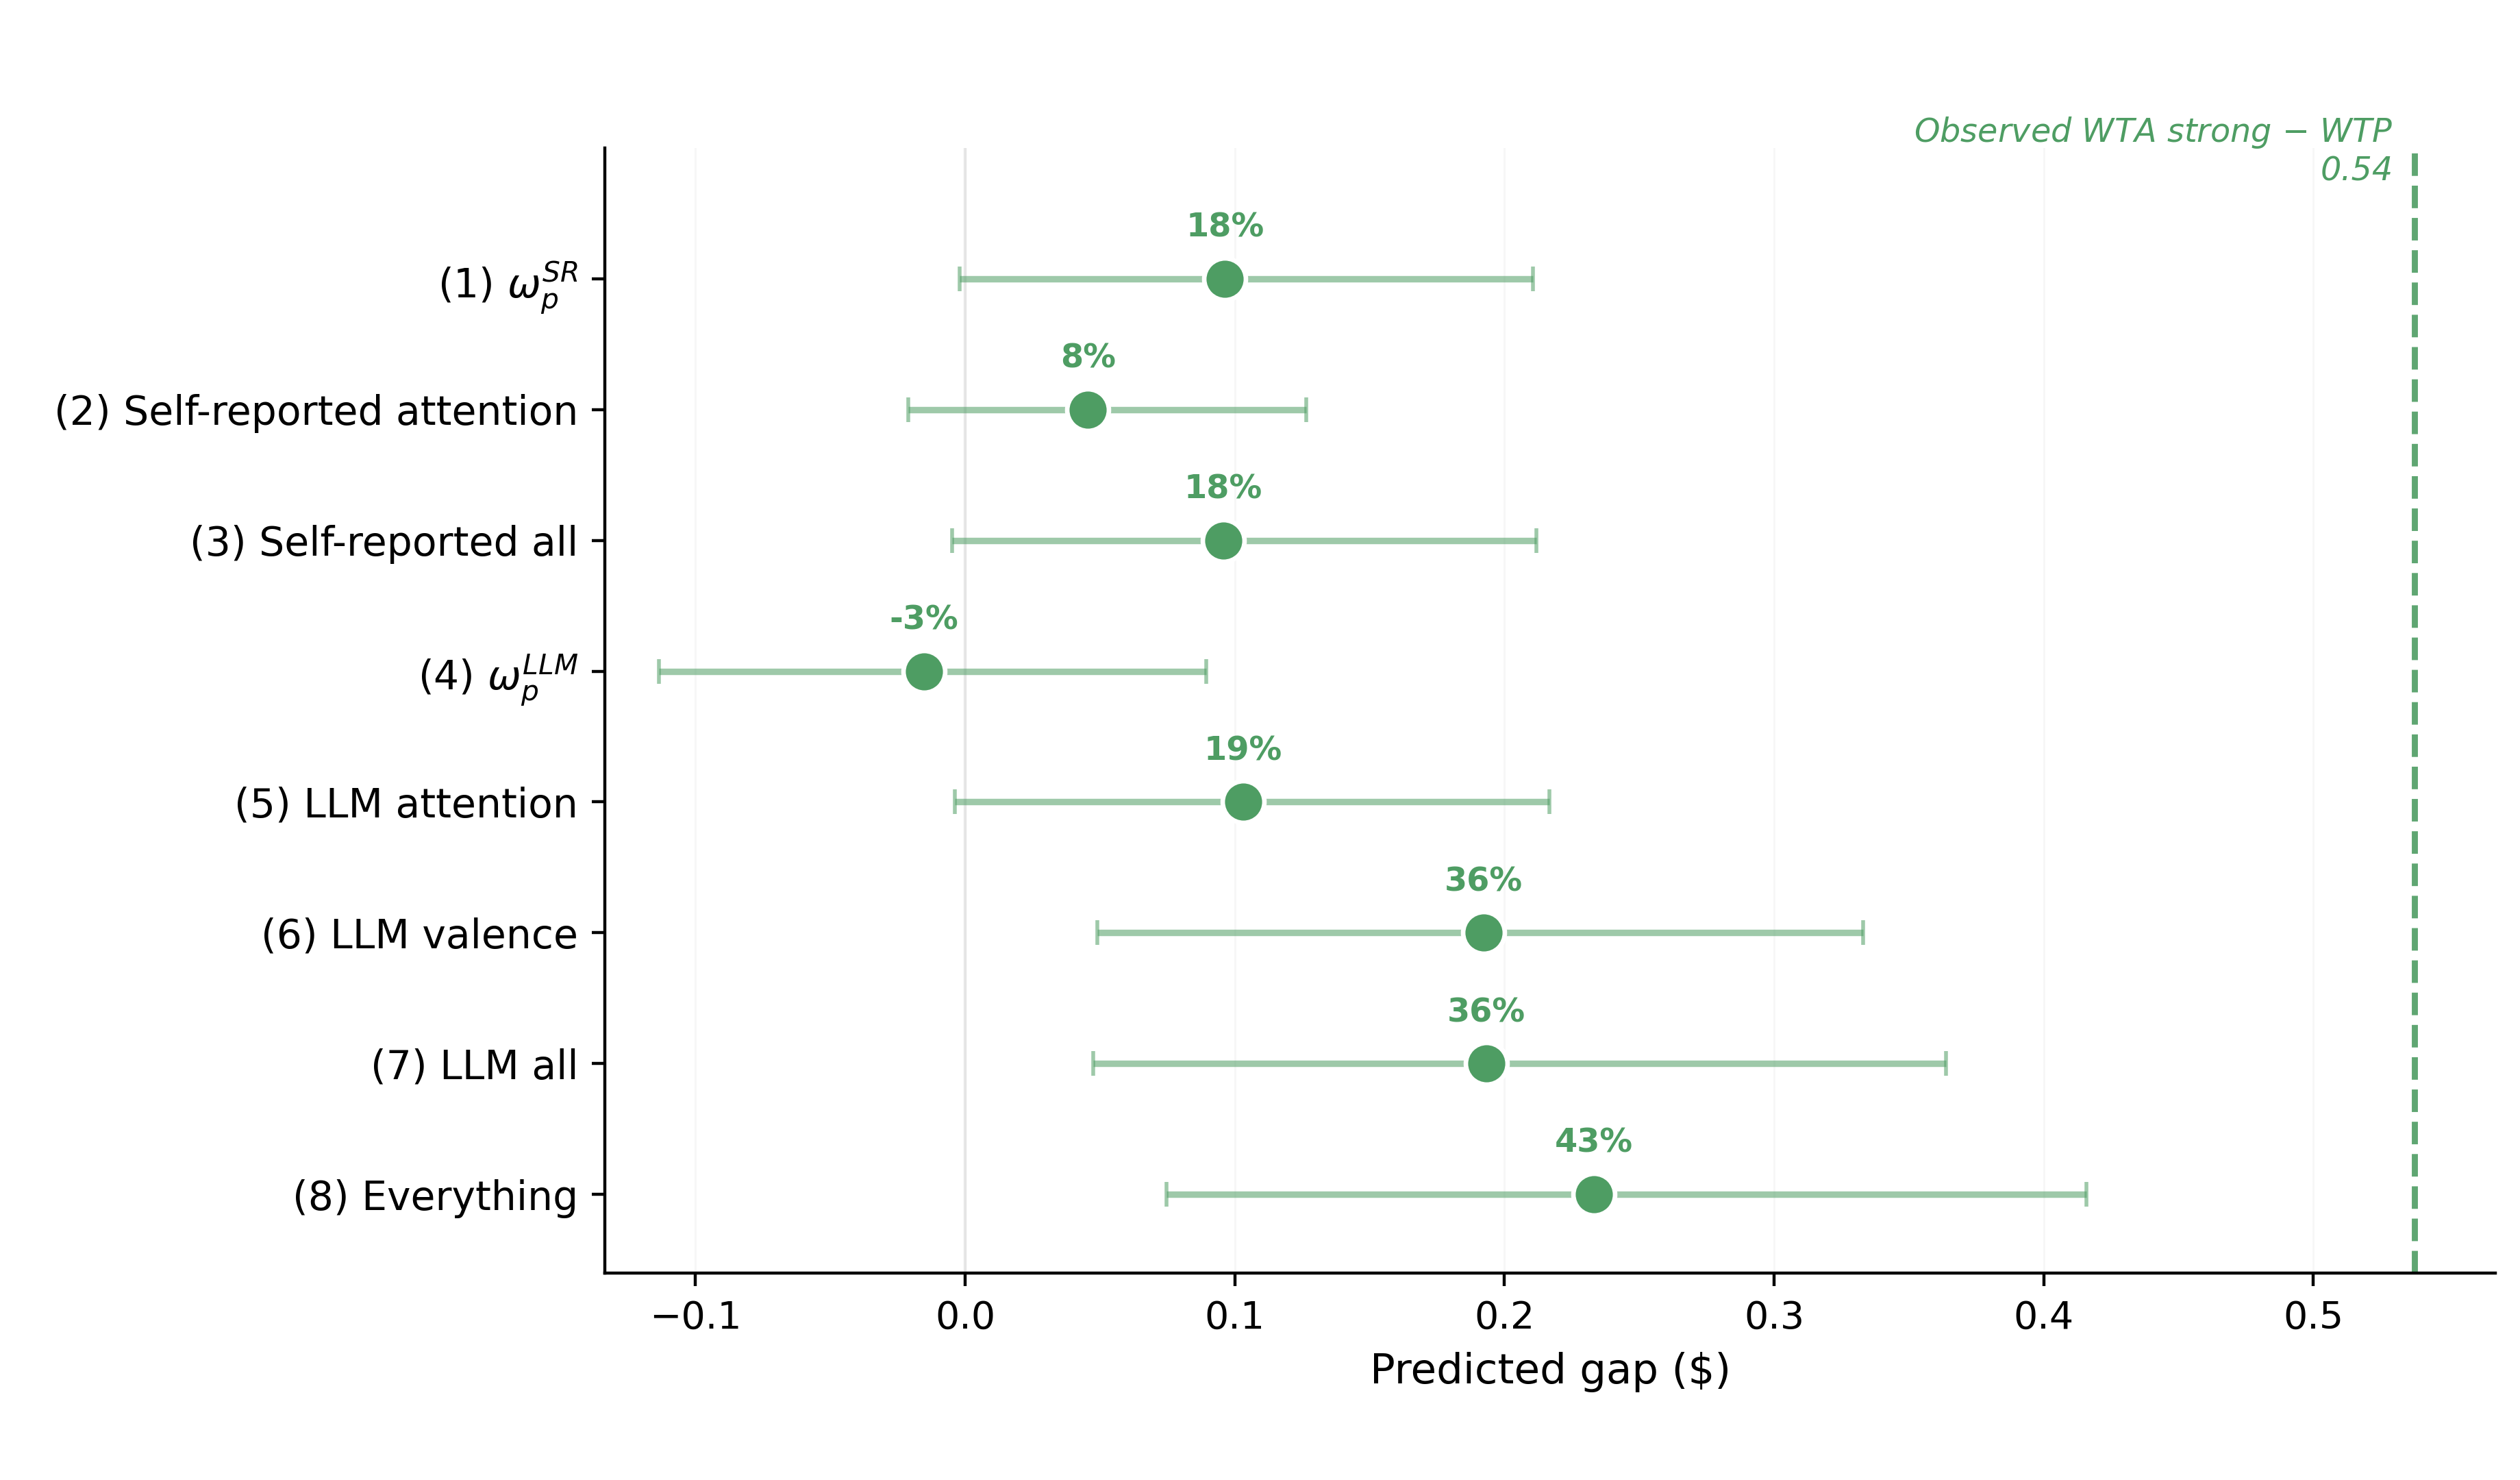
\includegraphics[width=0.92\linewidth,trim=0 6pt 0 10pt,clip]{figures/fig_gap_actual_predicted_strong.png}
 
\vspace{2pt}
{It pays off to combine both text and categorical reasoning.
\par}
 
\end{frame}

\begin{frame}{Appendix: Binary attention, multiple-choice version}
  \hypertarget{app:binary_attention_multiple_choice}{}
  \backbutton{main:binary_attention}
  \vspace{0.2cm}
  \begin{columns}
    \column{0.5\textwidth}
    \centering
    Cookies\\[2pt]
    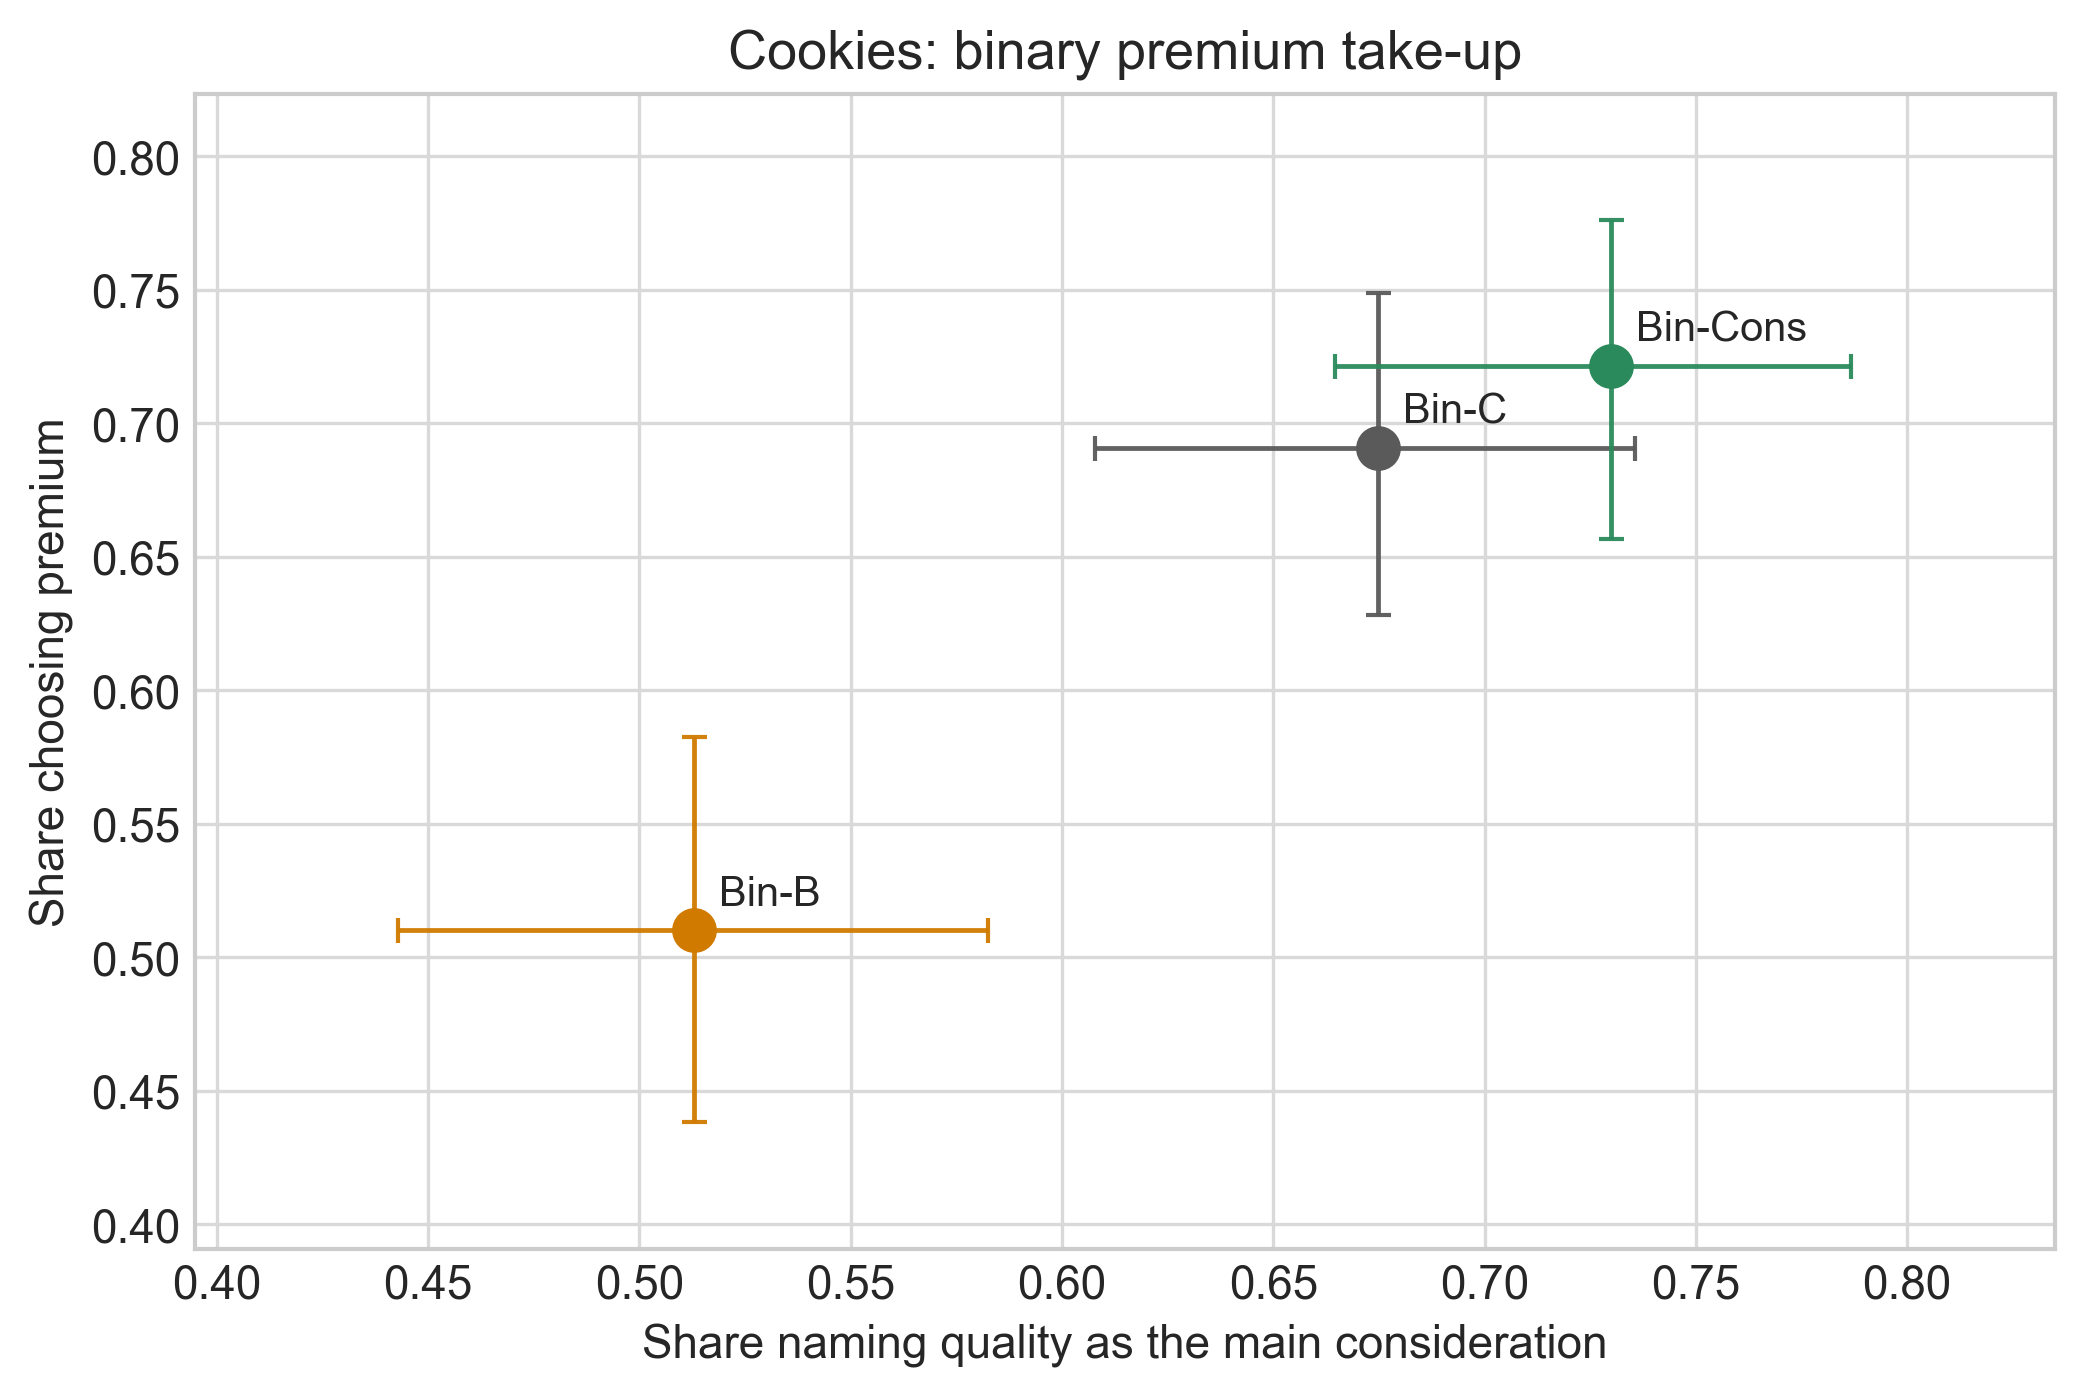
\includegraphics[width=\textwidth]{figures/binary_cookies_quality_share_vs_premium_share.png}

    \column{0.5\textwidth}
    \centering
    Toothpaste\\[2pt]
    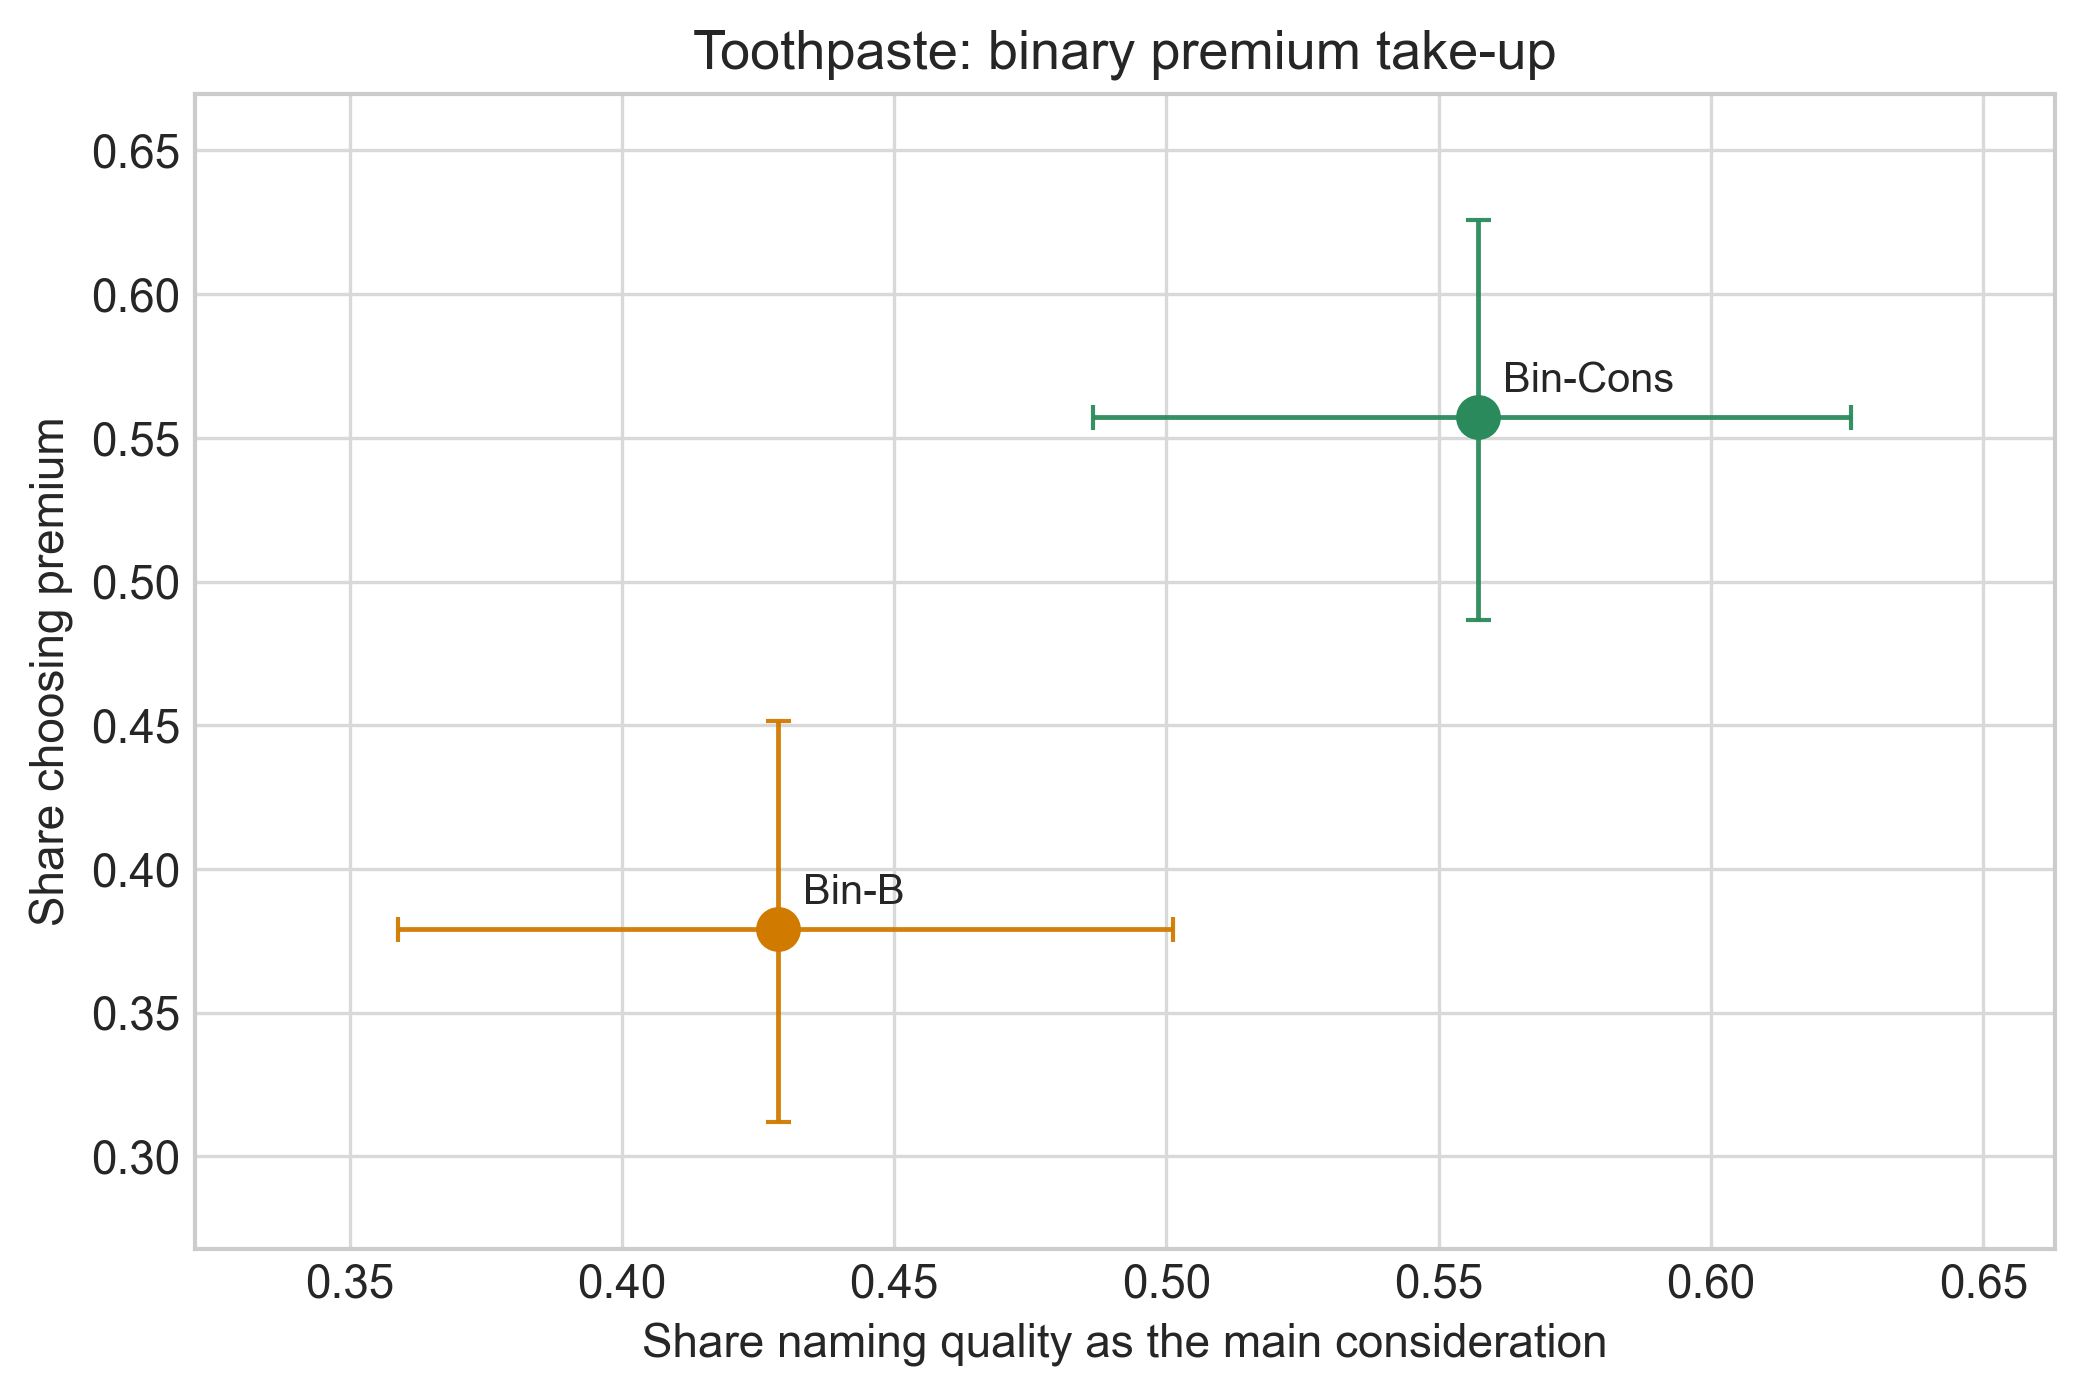
\includegraphics[width=\textwidth]{figures/binary_toothpaste_quality_share_vs_premium_share.png}
  \end{columns}
\end{frame}

\begin{frame}{Appendix: Cross-condition attention, multiple-choice version}
  \hypertarget{app:cross_attention_multiple_choice}{}
  \backbutton{main:cross_attention}
  \vspace{0.2cm}
  \begin{columns}
    \column{0.5\textwidth}
    \centering
    Cookies\\[2pt]
    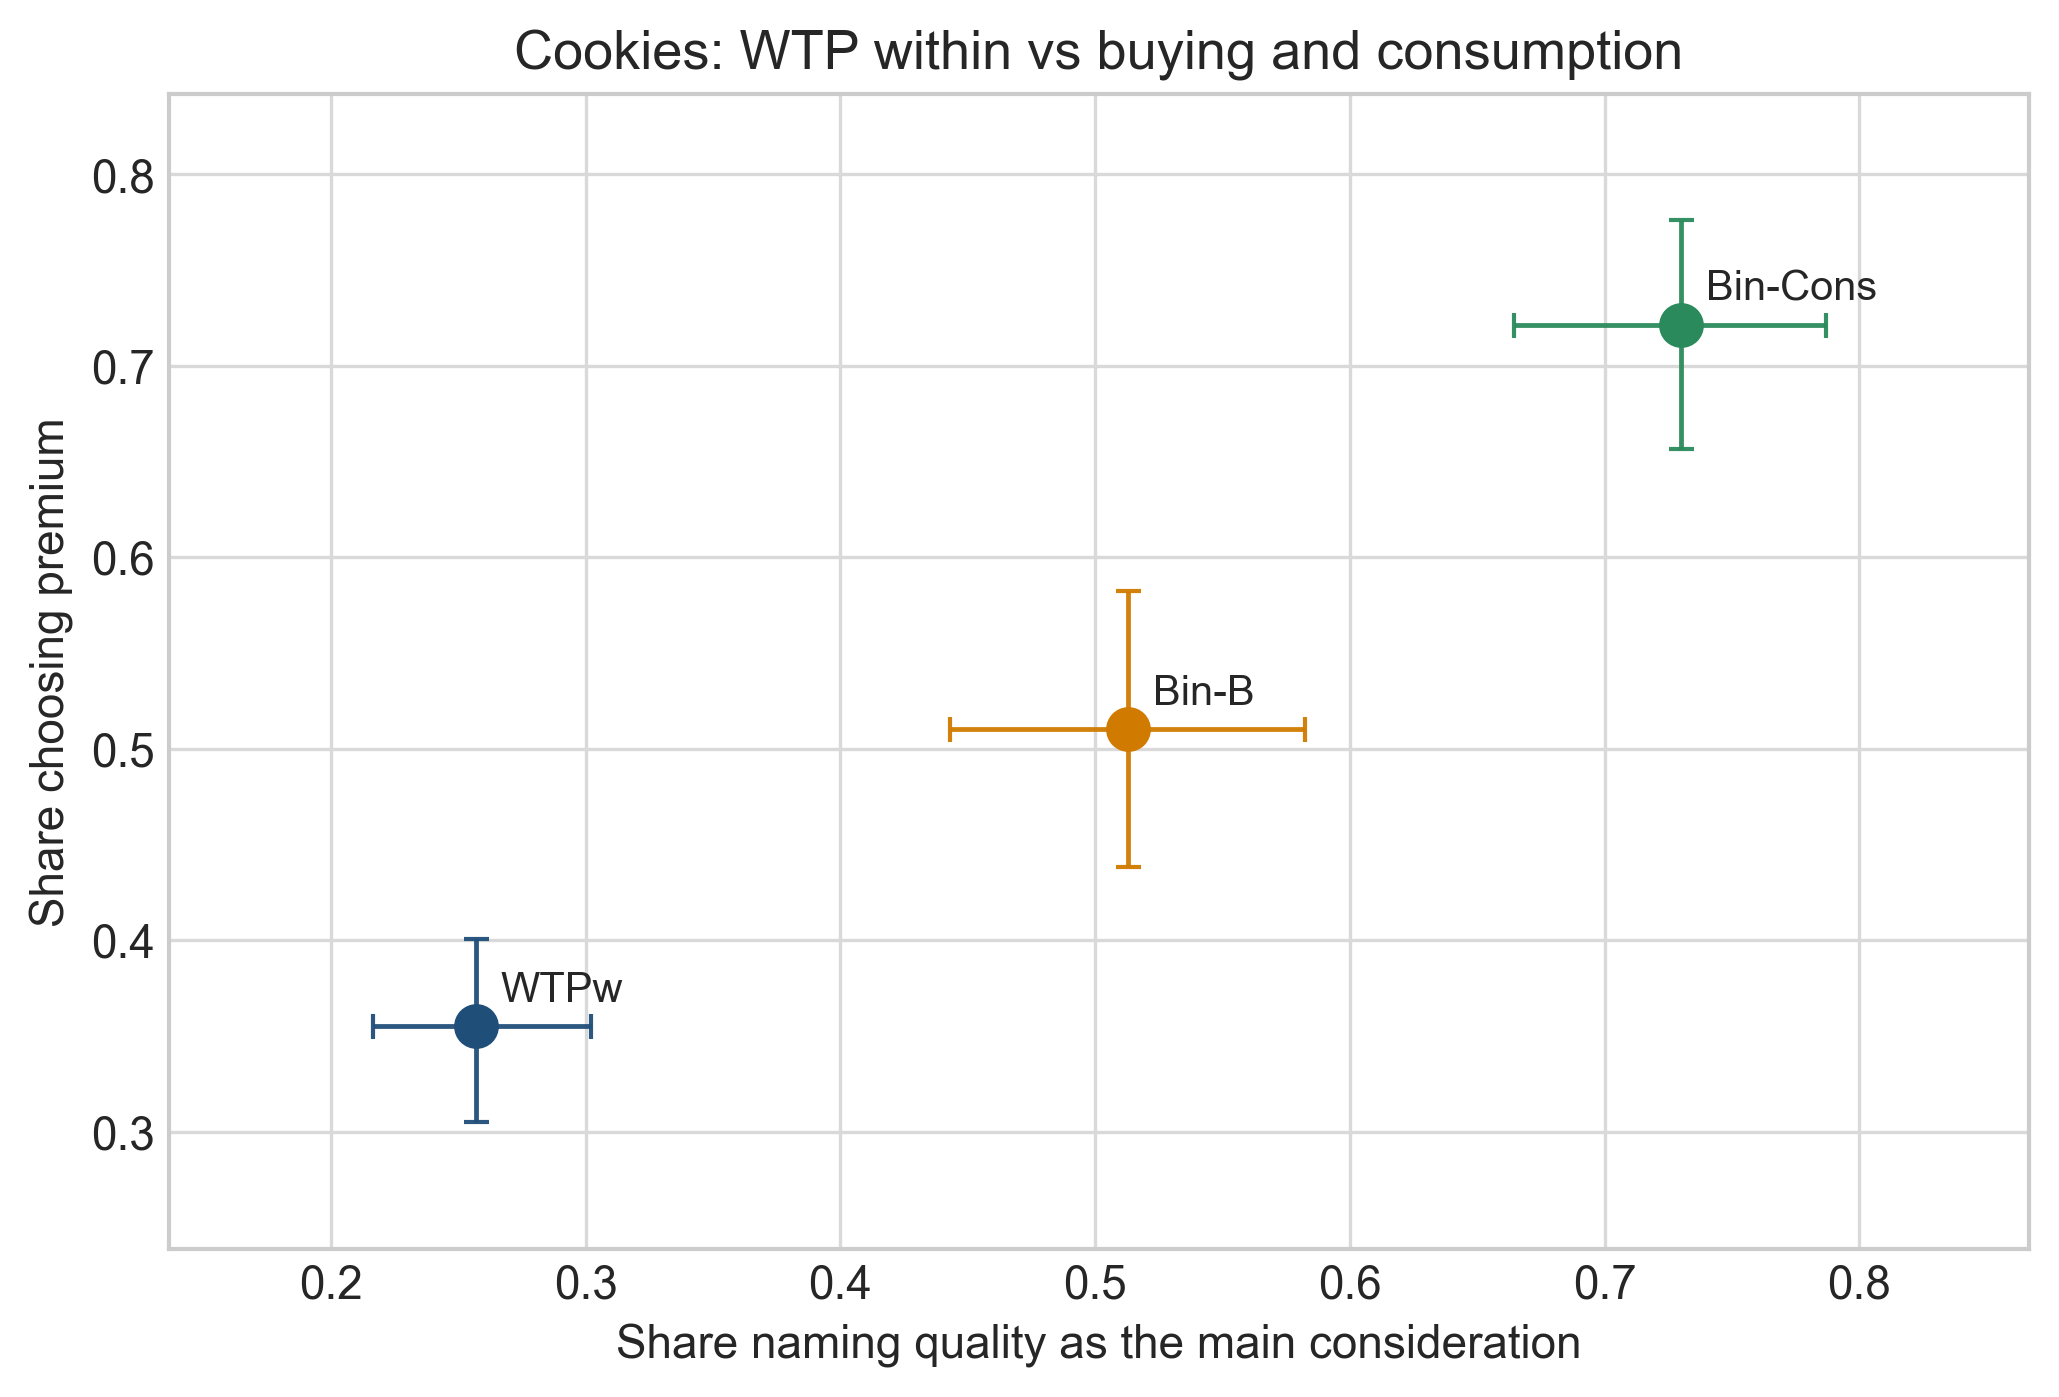
\includegraphics[width=\textwidth]{figures/cross_condition_cookies_quality_share_vs_premium_share.png}

    \column{0.5\textwidth}
    \centering
    Toothpaste\\[2pt]
    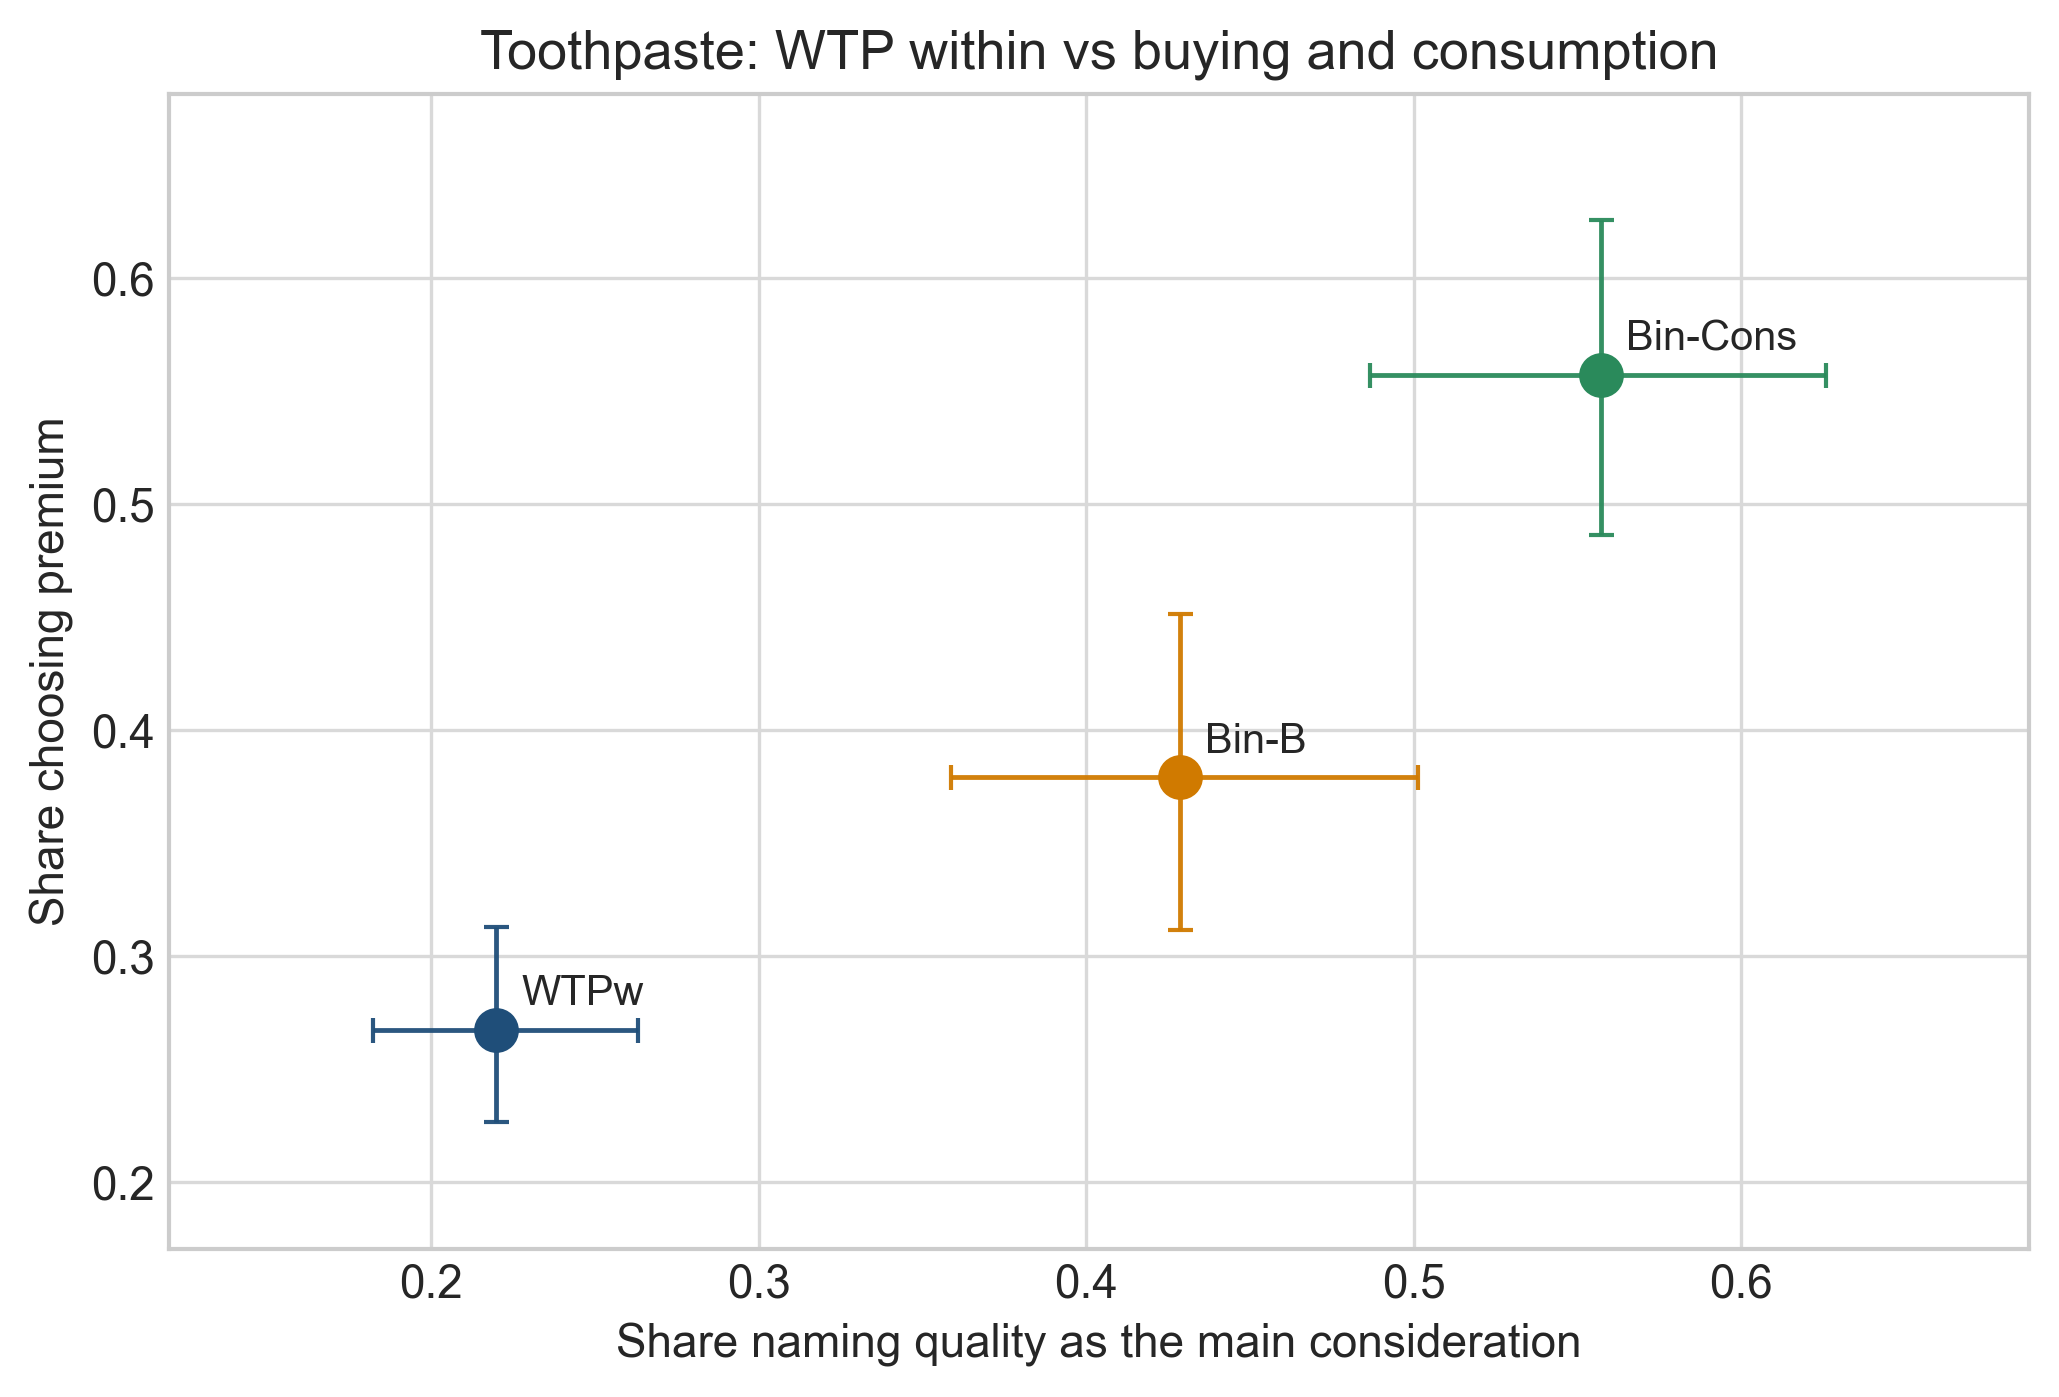
\includegraphics[width=\textwidth]{figures/cross_condition_toothpaste_quality_share_vs_premium_share.png}
  \end{columns}
\end{frame}


\begin{frame}[label=llm_finetune]{LLM price weight measure: fine-tuned model}
  A small model (GPT-4.1-mini) taught on reasoning texts, fixing:
  \begin{itemize}
    \item[$\bullet$] 75 is nearly 80, not fully wrong, the model needs to know some answers are closer than others.
    \item[$\bullet$]
      benefits from being shown how a stronger model reads the text (explicitly elicited LLM reasoning)
  \end{itemize}
\medskip
  \begin{enumerate}
    \item Group answers into 10 buckets (weight 65 falls in bucket 6),
      so nearby answers are treated as close.
    \item Show the model how to think first. Before the answer, add
      a short read of the text written by a smarter model (GPT-5).
    \item Teach it. Train on 3500 examples of ``text $\to$ read (from superior LLM)
      $+$ bucket (from human)''.
    \item Turn guess back into a number (final price weight from LLM). From model's distribution over buckets, take expected price weight.
  \end{enumerate}
  \backbutton{results_llm}
\end{frame}



\begin{frame}{LLM price weight measure: fine-tuned model performance}
  \begin{columns}[c]
    \column{0.55\textwidth}
      \centering
      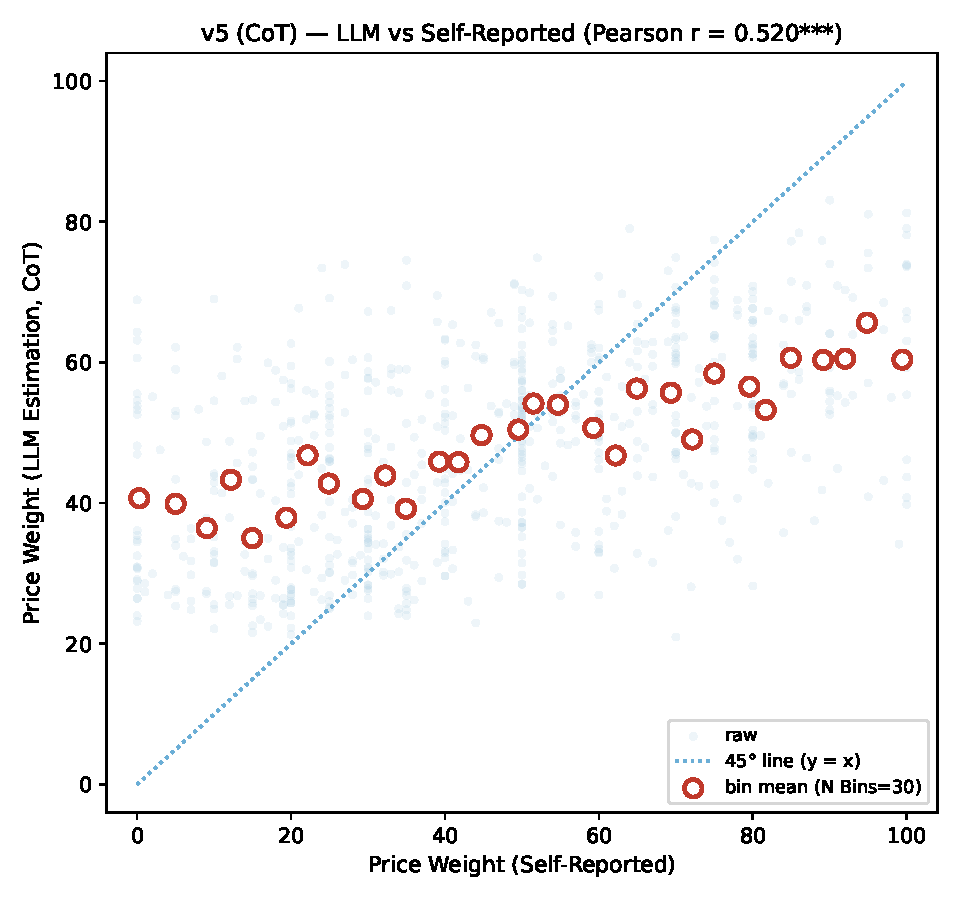
\includegraphics[width=\textwidth]{figures/fig1_v5_llm_sr_fit.pdf}
    \column{0.45\textwidth}
      \small
      \setlength{\tabcolsep}{4pt}
      \begin{tabular}{@{}lcc@{}}
        \toprule
        Metric & Prompted & Fine-tuned \\
        \midrule
        $N$                 & 4257  & 689 \\
        MAE                 & 33.35 & 18.11 \\
        RMSE                & 41.05 & 22.91 \\
        Pearson $r$         & $0.375^{***}$ & $0.520^{***}$ \\
        $R^2$ ($r^2$)       & 0.141 & 0.270 \\
        \bottomrule
      \end{tabular}
  \end{columns}
\end{frame}


% LLM classification prompt -- plainest beamer, no box, no special packages.


% ============================================================
% LLM classification prompt -- plain beamer with paragraph spacing.
% No box, no special packages.
% ============================================================

\begin{frame}{LLM classification prompt}
\small
You are an expert in text classification. Below is a respondent's reasoning for their choice.

\medskip
Respondent ID: \texttt{\{response\_id\}}. Response text: \texttt{\{text\}}.
\medskip
Assign the reasoning THREE outputs:
\begin{itemize}
\item a focus label (Price / Quality / Both);
\item a continuous weight on a 0--100 spectrum (0 = Quality, 100 = Price), measuring the quality--price trade-off;
\item a quality valence (``high'' / ``low'' / null) and a price valence (``high'' / ``low'' / null).
\end{itemize}

\medskip
\small
Output a single valid JSON object with no additional text:

\vspace{4pt}
{\ttfamily\scriptsize
\{\{ \\
\hspace*{1em}"ResponseId": "\{response\_id\}", \\
\hspace*{1em}"rel\_reasons\_gpt": "Price (Alternatives or Disutility)" \\
\hspace*{2.6em}or "Price (Reference Price)" or "Quality" \\
\hspace*{2.6em}or "Both" or "No cookie", \\
\hspace*{1em}"price\_weight\_gpt": \textless int 0--100, null if "No cookie"\textgreater, \\
\hspace*{1em}"quality\_valence\_gpt": "high" or "low" or null, \\
\hspace*{1em}"price\_valence\_gpt": "high" or "low" or null \\
\}\}
\par}

\end{frame}

\begin{frame}{LLM classification prompt}
\small
\textbf{Note:}

\begin{itemize}
\item Follow the classification rules carefully. Your judgment should make an effort to understand the respondent's reasoning.
\item Base your decision only on what the respondent actually wrote, and do not infer beyond it.
\item Price-focused answers are divided into ``Price (Alternatives or Disutility)'' and ``Price (Reference Price)''. The former means people mention using the money to buy other things or emphasize the pain of paying. Price-related responses without these two aspects, but still primarily about price, are labeled ``Price (Reference Price)''.
\item Classify as ``No cookie'' if and only if the text explicitly states ``No cookie.'' Otherwise it must be ``Price (Alternatives or Disutility)'', ``Price (Reference Price)'', ``Quality'', or ``Both''.
\end{itemize}
\end{frame}

\begin{frame}{LLM classification prompt}
\small
\textbf{Note (continued):}

\begin{itemize}
\item Continuous price weight from 0 to 100, using the same criteria as the focus label. 0 = purely quality-driven (a perfect match with the Quality criteria); 100 = purely price-driven (a perfect match with either Price criteria). Many responses are a mixture; infer the weight and assign a value between 0 and 100 based on how closely the logic aligns with each side.
\item Avoid defaulting to 50 when the response is short or ambiguous. Commit to the side the wording leans toward, even if weakly.
\item Valence rules: (i) if focus = ``Quality'', fill \texttt{quality\_valence\_gpt}, set \texttt{price\_valence\_gpt} to null. (ii) if focus = ``Price (Alternatives or Disutility)'' or ``Price (Reference Price)'', fill \texttt{price\_valence\_gpt}, set \texttt{quality\_valence\_gpt} to null. (iii) if ``Both'', fill both. (iv) if ``No cookie'', both null.
\end{itemize}
\end{frame}

\begin{frame}{LLM classification prompt}
\small
\textbf{A. Price (Alternatives or Disutility).}

\medskip
\emph{Rule:} label here if the reasoning mentions (i) using the money for something else / buying other items (opportunity cost) / switching options, or (ii) the pain of paying, not wanting to spend, or aversion to spending.

\medskip
\emph{Keywords, alternatives:} ``I could buy X instead'', ``spend the money on\ldots'', ``make it at home for cheaper''.

\medskip
\emph{Keywords, disutility:} ``don't want to spend more than\ldots'', ``wouldn't pay that much'', ``not worth spending'', ``just a treat so I won't spend much'', ``overpriced''.

\medskip
\textbf{Examples:}
\begin{itemize}
\item ``I thought about other potential options I could purchase.''
\item ``I could pay the same \$6 for something I like better.''
\item ``If I'm not happy with the price, I'll shop elsewhere or purchase a store brand instead.''
\item ``I don't want to shell out much more than a dollar\ldots''
\item ``I don't need them and wouldn't pay regular price.''
\end{itemize}
\end{frame}

\begin{frame}{LLM classification prompt}
\small
\textbf{B. Price (Reference Price).}

\emph{Rule:} label here if the reasoning mainly mentions reference price, usual cost, a reasonable price, a price guessed from store norms, quantity, or unit-price math (``only 12 cookies'', ``price per cookie'', ``small package so lower price''), and does \emph{not} mention (i) buying something else instead or (ii) the pain of paying / not wanting to spend.
\medskip

\textbf{Examples:}
\begin{itemize}
\item ``I tried to remember how much a package \ldots usually costs.''
\item ``I don't buy cookies so I don't know the price. I just guessed \ldots''
\item ``I was thinking that it is only 12 cookies\ldots''
\item ``33 cents a cookie seems fair.''
\item ``I thought about how much I think these cookies cost in the store.''
\end{itemize}
\end{frame}

\begin{frame}{LLM classification prompt}
\small
\textbf{C. Quality.}
\medskip
\emph{Rule:} classify as ``Quality'' if the reasoning mainly centers on taste, ingredients, freshness, whether the product is handmade, how good it is, how premium it feels, or how healthy it is.
\medskip


\emph{Keywords:} taste / delicious / flavorful; quality / high / low; ingredients / organic / processed; homemade / fresh / artisanal; brand reputation; texture (soft / dry / crumbly); health / unhealthy; packaging as a quality signal; novelty / experience.
\medskip

\textbf{Examples:}
\begin{itemize}
\item ``I would consider the taste and quality. Tate's cookies are known for being crisp and flavorful.''
\item ``These cookies are delicious and I would pay a premium price for them.''
\item ``They look home made and soft and creamy.''
\item ``I do not like these cookies. They are hard and the chocolate tastes bitter.''
\item ``Tate's is a premium brand and usually costs more because of the quality and packaging.''
\item ``I love Tate's cookies. They are so good!''
\end{itemize}
\end{frame}
\medskip

\begin{frame}{LLM classification prompt}
\small
\textbf{D. Both.}

\emph{Rule:} assign ``Both'' only when a price consideration and a quality consideration are genuinely weighed against each other. A quality word that merely endorses the price (``good cookies at a fair price'') is not weighing.
\medskip


\emph{Signals:} explicit trade-off language (``balance'', ``weighed X against cost'', ``quality vs price''); quality pulls the price up while price or budget pulls it back, neither dominant (``good quality, but I won't pay more than \$5'').
\medskip

\textbf{Examples:}
\begin{itemize}
\item ``Five dollars feels like it's expensive enough that the quality is good, but not too expensive where it feels overpriced.''
\item ``Tate's cookies are good though and better quality, so if they were under \$5 I may buy them.''
\item ``My decision was based on the balance between expected enjoyment, brand familiarity, and whether the price felt reasonable for that level of quality.''
\item ``It's a quality brand, but you are getting few cookies for your money\ldots \$5 is a lot to pay for maybe 10 cookies.''
\end{itemize}
\end{frame}

\begin{frame}{LLM classification prompt}
\small
\textbf{E. Valence levels.}
Do NOT use the respondent's final price or any reference to the \$5 anchor as a signal.
\medskip

\textbf{Quality valence} (if focus = Quality or Both):
\begin{itemize}
\item ``high'': product described as good, delicious, premium, fresh, well-made, or appealing.
\item ``low'': product described as poor, bland, processed, unhealthy, or unappealing.
\end{itemize}
\medskip
\vspace{-1em}

\emph{High:} ``These cookies are delicious.''; ``Tate's is a premium brand.''; ``Soft and creamy.'' 
\medskip

\emph{Low:} ``Hard and bitter.''; ``Heavily processed.''

\vspace{6pt}
\textbf{Price valence} (if focus = Price (Alt.\ or Disutility), Price (Reference), or Both):
\vspace{-1em}
\begin{itemize}
\item ``high'': price described as expensive or steep, in general terms.
\item ``low'': price described as cheap, affordable, or fair, in general terms.
\end{itemize}
\emph{High:} ``Cookies like these are pricey.''; ``Overpriced in general.''; ``Premium products cost a lot.'' 

\medskip
\emph{Low:} ``Cookies are usually cheap.''; ``Affordable snack.''; ``Reasonably priced.''
\end{frame}



\end{document}
